%!TEX root = ../main.tex

\chapter{The background before analysis cuts}\label{chap:bkg:raw:ph2}

As already mentioned, a precise knowledge of background intensity and distribution is
essential to searches of faint signals. One main assumption of the \onbb-decay signal
analysis is the distribution of background events in the analysis window around \qbb\
being uniform, except for the known \Tl\ and \Bil\ \g\ lines. The primary role of the
background model is to verify this assumption by exploiting data outside this energy
region or filtered with a different event selection. The background model is also
complementary to assay measurements in determining the location of the most dangerous
background sources and learn how to improve experimental design and material selection in
similar future projects. Lastly, a good background model allows to isolate \nnbb-decay
events, estimate the half-life of the process and study their distribution as a source of
potential new-physics effects (see \cref{chap:theory}).
\newpar
A first background model has been built for the \phaseone\ data and published
in~\cite{Agostini2013a}. Later, a new and advanced model has been constructed to describe
the first 60~\kgyr\ of \phasetwo\ data before the LAr veto and PSD cuts, which has been
published in~\cite{Agostini2019b} and is described in detail in this chapter. In
\cref{sec:bkg:raw:ph2:data} the selected data is presented and characterized, while the
procedure to compute the theoretical expectations used in the statistical analysis is
outlined in \cref{sec:bkg:raw:ph2:pdfs} (the topic is addressed in more detail in
\cref{apdx:magepdfs}). The prior knowledge about the presence of contaminants in the
\gerda\ setup that contribute to the germanium background spectrum is summarized in
\cref{sec:bkg:raw:ph2:priors}. The statistical framework and the analysis strategy is
presented in \cref{sec:bkg:raw:ph2:stat}. As it will be shown, the high-statistic \kvn,
\kvz\ and \a\ event data samples deserve dedicated studies and are thus treated
separately. These potassium and \a\ event analyses are presented in
\cref{sec:bkg:raw:ph2:kmodel} and \cref{sec:bkg:raw:ph2:amodel} respectively. Finally, the
results of the background decomposition in the full energy range are given in
\cref{sec:bkg:raw:ph2:gmodel} and discussed in \cref{sec:bkg:raw:ph2:discussion}.

\section{Analysis data sets}%
\label{sec:bkg:raw:ph2:data}

\begin{figure}
  \centering
  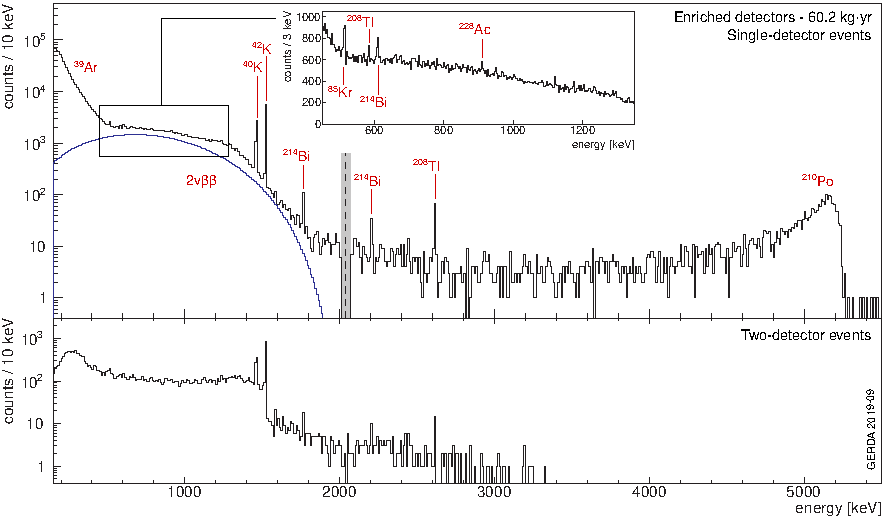
\includegraphics[width=0.9\linewidth]{plots/bkg/raw/ph2/dataGe-desc.pdf}
  \caption{%
    Summed energy spectra of single-detector events (\enrBEGeII\ and \enrCoaxII, top
    panel) and two-detector events (\enrGeII, bottom panel) collected in \gerda\
    \phasetwo.  The prominent features due to detector intrinsic \nnbb\ events, \kvz,
    \Arl\ and \Kr\ in the LAr, \kvn, the \Thh\ and \Uh\ decay chains are highlighted. The
    window blinded for the \onbb\ analysis is marked in grey.
  }\label{fig:bkg:raw:ph2:datasets}
\end{figure}

\begin{table}
  \centering
  \caption{%
    Properties of the data sets considered in this analysis. Further
    details about the \gerda\ detectors can be found in past
    publications~\cite{Agostini2013a, Agostini2018a}. \fillme{check with Katharina}
  }\label{tab:bkg:raw:ph2:datasets}
  \small
  \begin{tabular}{lccccc}
  \toprule
  \mr{2}{data set} & \mr{2}{composition}     & total Ge           & active \gesix\   & total Ge           & active \gesix\     \\
                   &                         & mass (kg)          & mass (kg)        & exposure (\kgyr)   & exposure (\kgyr)   \\
  \midrule
  \enrBEGeIIp\     & 29 \bege\footnotemark{} & $19.362 \pm 0.005$ & $17.17 \pm 0.32$ & $22.181 \pm 0.006$ & $17.31  \pm 0.32$  \\
  \enrSCoaxIIp\    & 6 \scoax\               & $11.827 \pm 0.002$ & $10.38 \pm 0.42$ & $13.179 \pm 0.003$ & $10.00  \pm 0.42$  \\
  \enrICoaxIIp\    & 4 \icoax\               & $ 7.802 \pm 0.002$ & $ 7.23 \pm 0.03$ & $ 8.775 \pm 0.002$ & $ 7.13  \pm 0.03$  \\
  \enrGeIIp\       & all enriched            & $38.991 \pm 0.006$ & $34.78 \pm 0.53$ & $44.135 \pm 0.007$ & $34.44  \pm 0.53$  \\
  \bottomrule
\end{tabular}

% vim: nowrap

\end{table}%
\footnotetext[1]{%
  The BEGe detector \GD{02D} is the only detector that does not fully
  deplete~\cite{Agostini2018a}. Hence, events triggered by this detector are
  not considered in either data set and it is omitted from the mass
  computation.
}

As already mentioned, the background model before cuts has been developed using data from
the first part of \phasetwo, namely, for data acquired starting from December 2015 to
March 2018. Single-detector (or multiplicity-one, abbreviated \Mone) events and
two-detector (multiplicity-two, abbreviated \Mtwo) events are considered for this
analysis. Events from the semi-coaxial detectors with natural isotope composition, located in
the central detector string, are not used in this analysis due to large uncertainties on
their \nplus\ contact thickness and detection efficiency. The \Mone\ events are split in
two data sets based on the two enriched detector geometries which we call \enrBEGeII\ and
\enrCoaxII\ in the following.  The \Mtwo\ data form a third data set which is named
\enrGeII. The energy we associate to an \Mtwo\ event is the sum of the energies
reconstructed in the two detectors. The data sets, their exposure and respective detector
mass are listed in \cref{tab:bkg:raw:ph2:datasets}. Note that the \bege\ exposure of
31.1~\kgyr\ is higher than the one reported in~\cite{Agostini2019a} because additional
data for which PSD methods are not applicable is here included.
\newpar
The event energy distribution of the three data sets is displayed in
\cref{fig:bkg:raw:ph2:datasets}: the sum spectrum of \enrBEGeII\ and \enrCoaxII\ in the
top panel and \enrGeII\ in the bottom panel. For the single-detector data, in the top
panel, the following features are most noticeable: the \b\ decay of \Arl\ dominates the
spectrum up to 565~keV while between 600 and 1500~keV the most prominent component is the
continuous spectrum of \nnbb\ decay of \gesix. Two \g\ lines at 1461 and 1525~keV can be
attributed to \kvn\ and \kvz; further visible \g\ lines belonging to \Kr, \Tl, \Bih\ and
\Ac\ are indicated in the figure. The highest energies displayed are dominated by a
peak-like structure emerging at 5.3~MeV with a pronounced low energy tail. This is a
typical spectral feature of \a\ particles and can, here, be attributed to \Po\ decay on
the thin detector \pplus\ surfaces~\cite{Agostini2013a}.  Events above the \Po\ peak
belong to \a\ decays emerging from the \Ra\ sub-chain on the detector \pplus\ surfaces.
All these components contribute also to \enrGeII\ except for \Arl, \nnbb\ and high energy
\a-components. This is due to the short range of \a\ (tens of \mum) and \b\
particles (typically smaller than 1.5~cm) in LAr and germanium with respect to the
distance between detectors which is of the order of several cm.

\section{Monte Carlo simulations and probability density functions}%
\label{sec:bkg:raw:ph2:pdfs}

The probability density functions (pdfs) used to model contributions to the energy spectra
are obtained from Monte Carlo simulations. The latter are performed using the \mage\
simulation framework~\cite{Boswell2011}, based on
\geant~\texttt{v10.4}~\cite{Agostinelli2002, Allison2006, Allison2016}.  \mage\ contains a
software implementation of the \gerdatwo\ detectors as well as the assembly and all other
surrounding hardware components. A visualization of this implementation is presented in
\cref{fig:setup:magevolumes}. Detector intrinsic \nnbb\ decays of \gesix\ and background
events originating from radioactive contaminations in and around the detector assembly are
simulated. The energy spectrum of the two electrons emitted in the \nnbb\ decay was
sampled according to the distribution given in~\cite{Tretyak1995} and implemented in
\decayzero~\cite{Ponkratenko2000}. The pdfs are obtained from the Monte Carlo simulations,
taking into account the finite energy resolution and individual exposure acquired with
each detector during the considered data taking periods. Special care is taken not to
statistically bias the pdfs by assuring that each simulated decay is taken into account
only once in the production of a pdf. For more details see \cref{apdx:magepdfs}. The
germanium detector active volume model is also applied to the simulations during this
post-processing step. A simplified step-like function that defines the charge-collection
efficiency (CCE) value depending on the depth from the detector surface is used to produce
the pdfs for the analysis of \phasetwo\ data before the upgrade. The CCE is set to a null
value through all the transition region between the surface and the full charge-collection
efficiency region. From the full charge-collection depth (FCCD) and below the CCE is set
equal to unity. The estimated FCCD values for each detector are documented and discussed
in \cref{apdx:gedetav}. The pdfs for the background model of \gerdatwo\ data before
cuts are displayed in
\cref{fig:bkg:raw:ph2:pdfs:gmodel,fig:bkg:raw:ph2:pdfs:amodel,fig:bkg:raw:ph2:pdfs:kmodel:K40,fig:bkg:raw:ph2:pdfs:kmodel:K42}
and will be presented in more detail in the following.

\section{Background expectations}%
\label{sec:bkg:raw:ph2:priors}

\begin{figure}
  \centering
  \subfloat[\label{fig:bkg:raw:ph2:pdfs:gmodel:Th}%
    \Bil\ and \Tl\ (\Thh\ chain) contaminations far from (fiber shroud) and close to
    (mini-shrouds) the detectors.
  ]{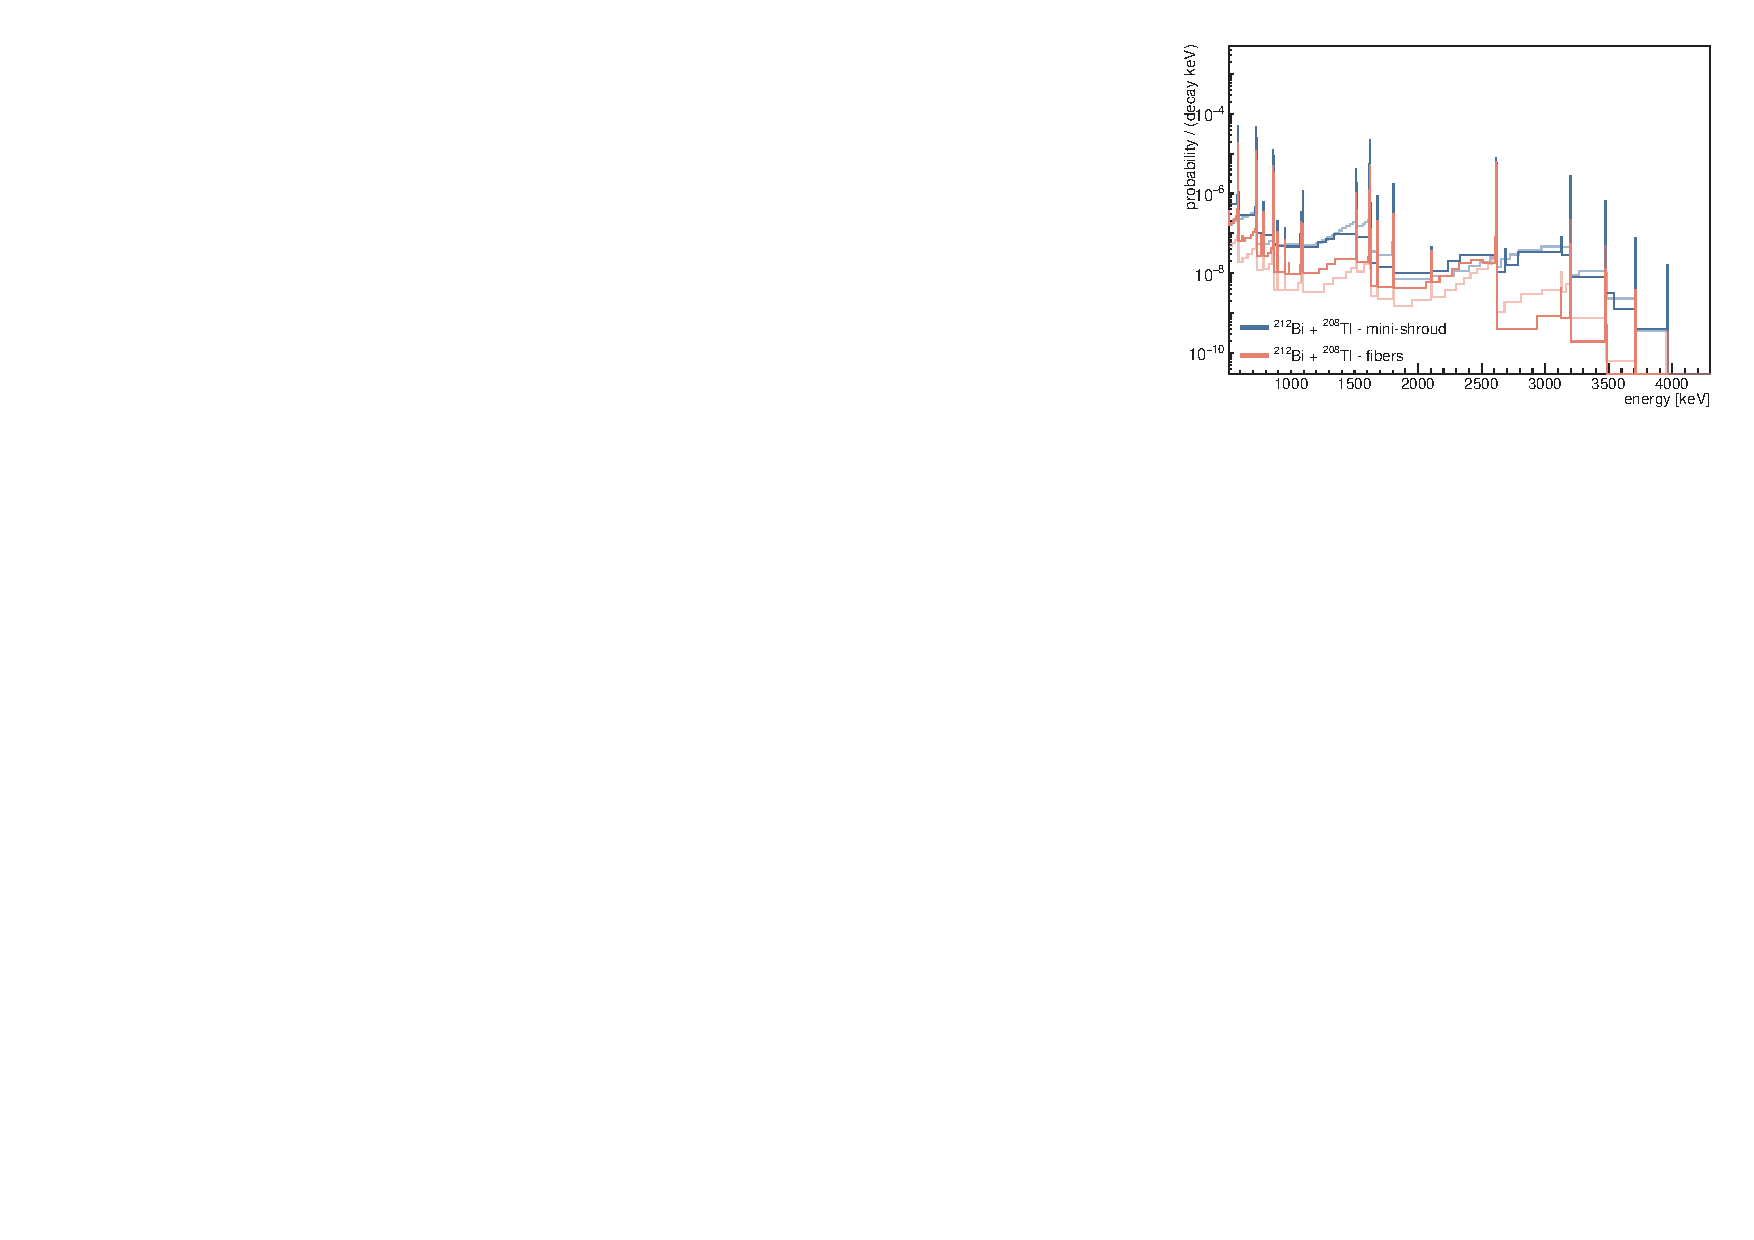
\includegraphics[width=0.48\textwidth]{plots/bkg/raw/ph2/pdfs/gmodel-pdfs-Th.pdf}}
  \hfill
  \subfloat[\label{fig:bkg:raw:ph2:pdfs:gmodel:U}%
    \Bih\ and \Pbh\ (\Uh\ chain) contaminations far from (fiber shroud) and close to
    (mini-shrouds) the detectors.
    ]{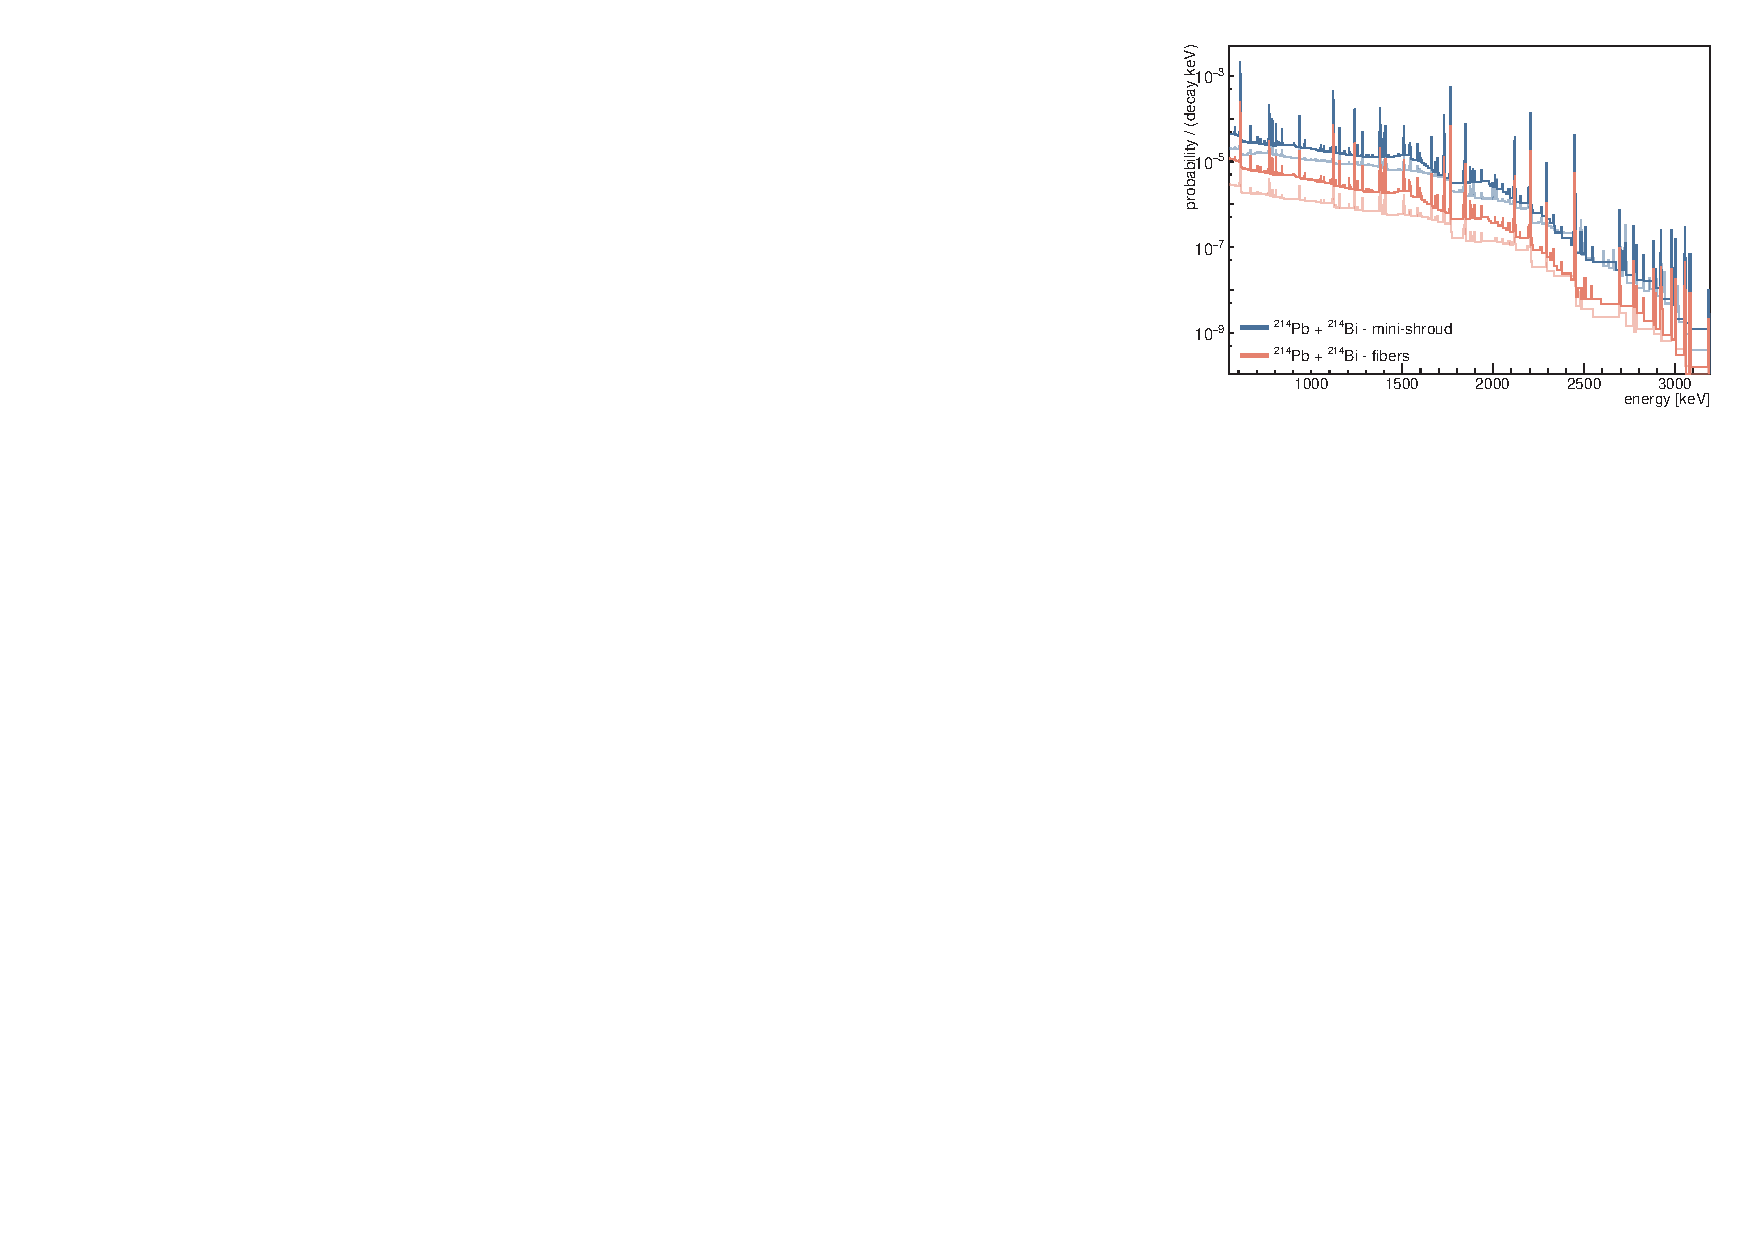
\includegraphics[width=0.48\textwidth]{plots/bkg/raw/ph2/pdfs/gmodel-pdfs-U.pdf}}

  \subfloat[\label{fig:bkg:raw:ph2:pdfs:gmodel:K40}%
    \kvn\ contamination close to the detectors (mini-shrouds), at a higher radial distance
    (fiber shroud) and higher vertical distance (copper shrouds).
  ]{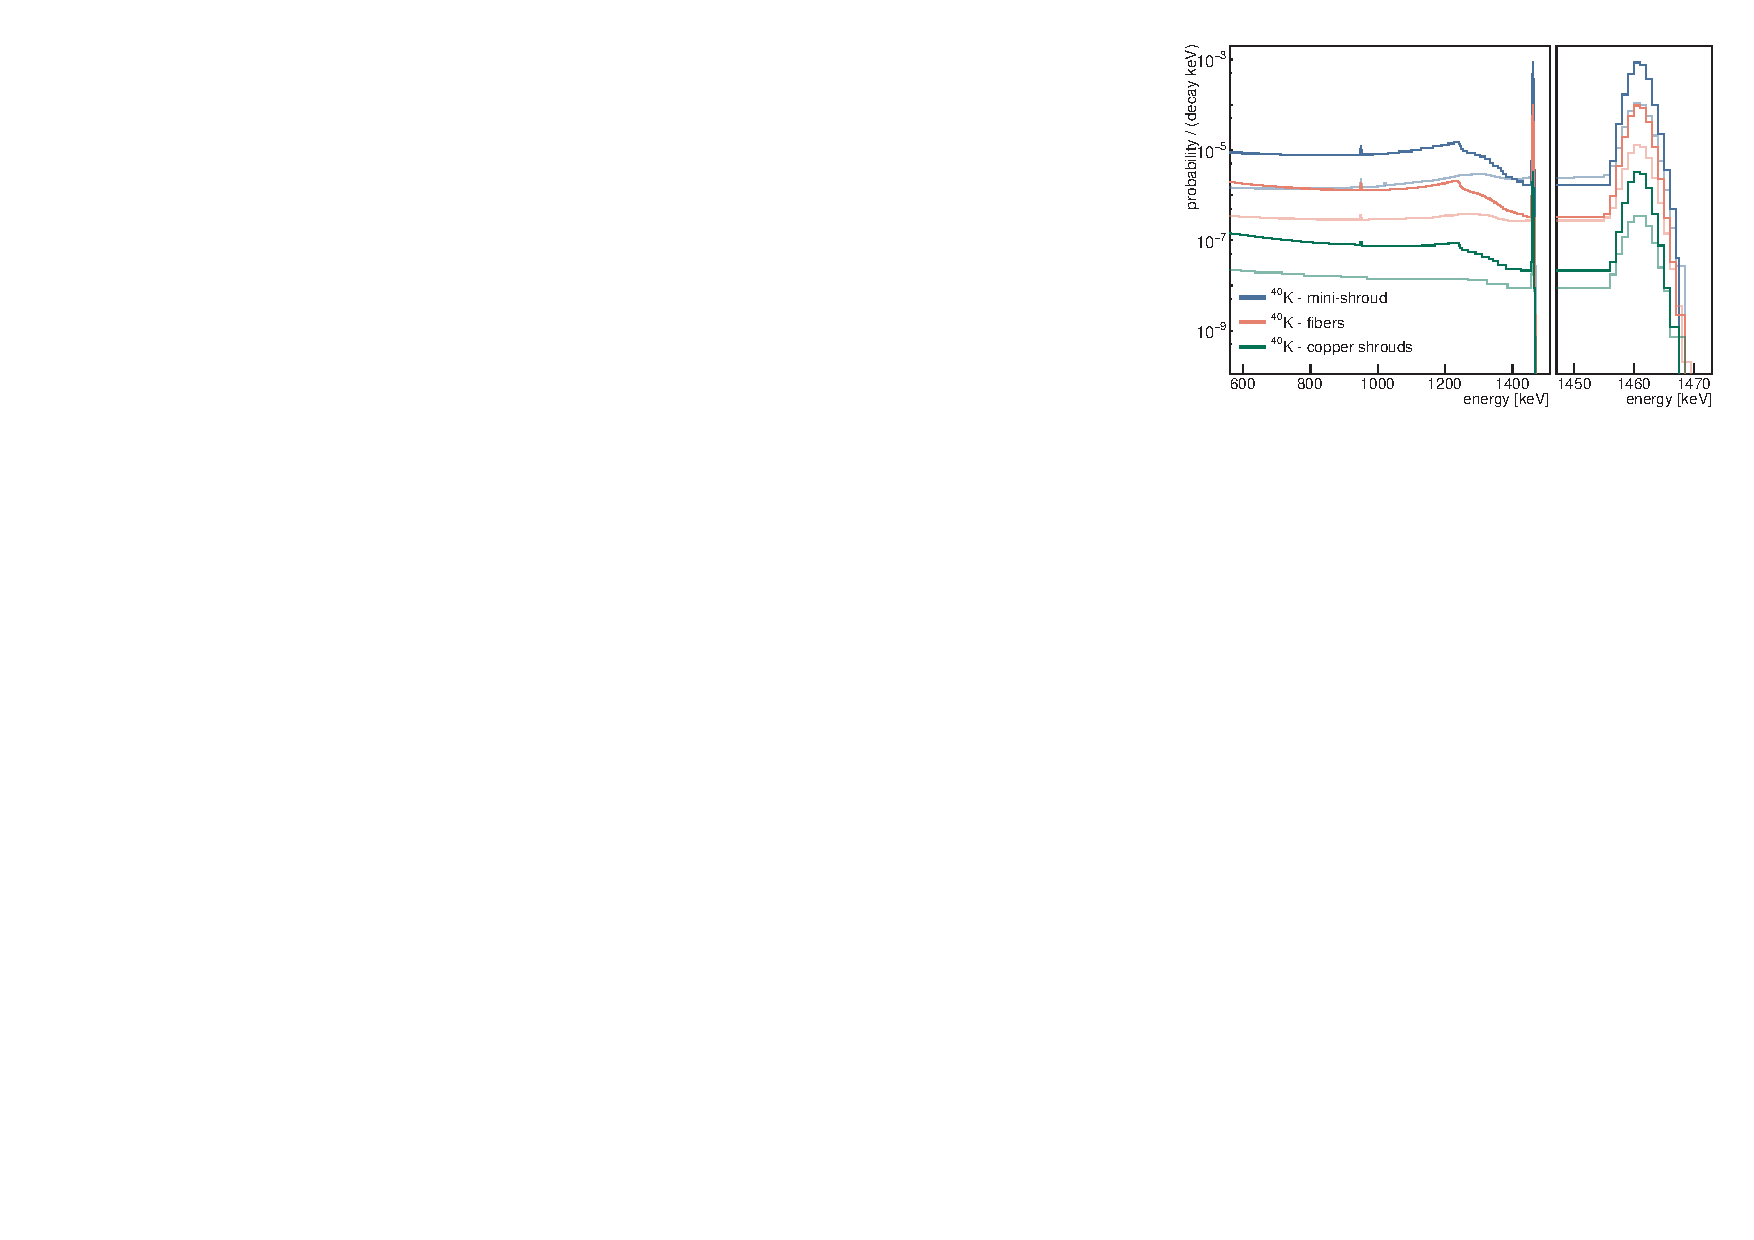
\includegraphics[width=0.48\textwidth]{plots/bkg/raw/ph2/pdfs/gmodel-pdfs-K40.pdf}}
  \hfill
  \subfloat[\label{fig:bkg:raw:ph2:pdfs:gmodel:K42}%
    \kvz\ contamination in different locations inside the LAr.
  ]{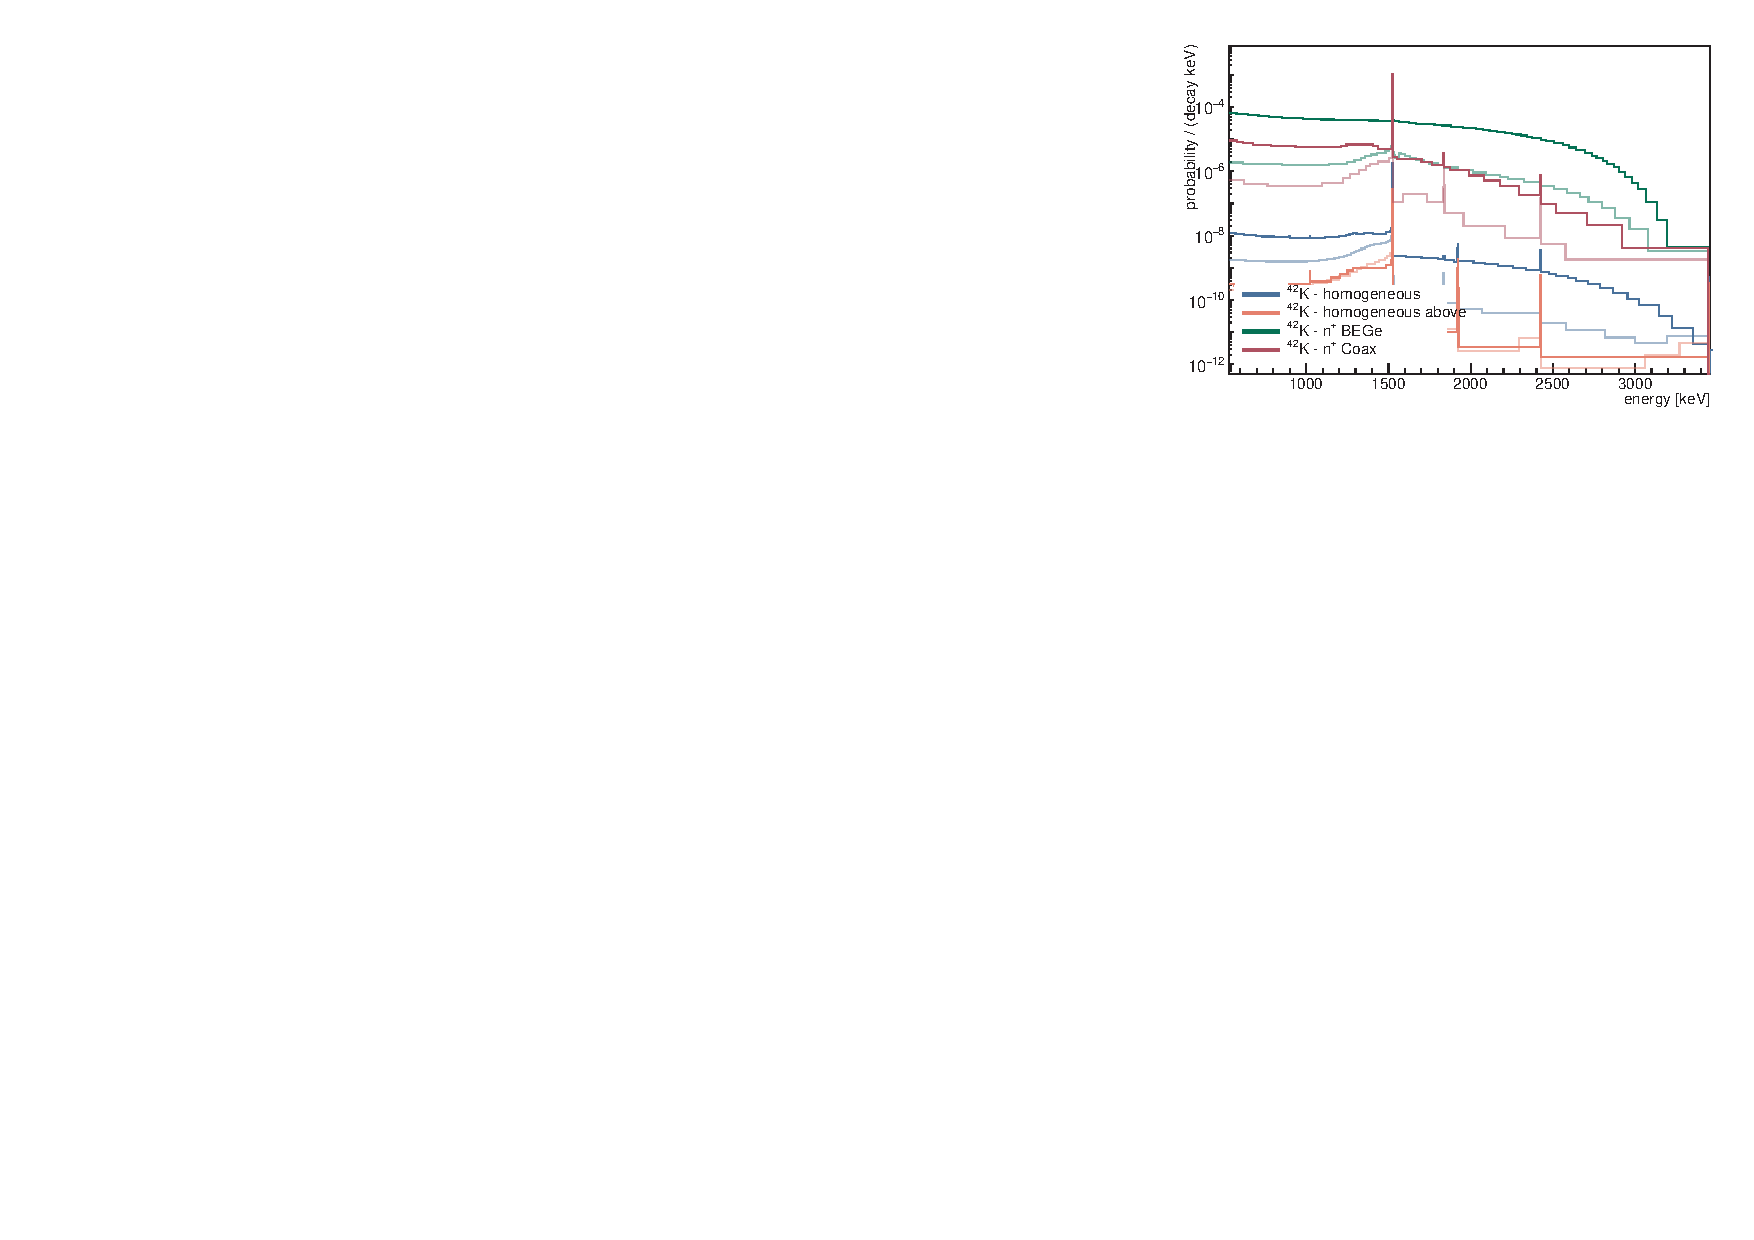
\includegraphics[width=0.48\textwidth]{plots/bkg/raw/ph2/pdfs/gmodel-pdfs-K42.pdf}} \\

  \subfloat[\label{fig:bkg:raw:ph2:pdfs:gmodel:other}%
  \Pa\ and \Ac\ contaminations in the close vicinity of the detectors (mini-shrouds).
  ]{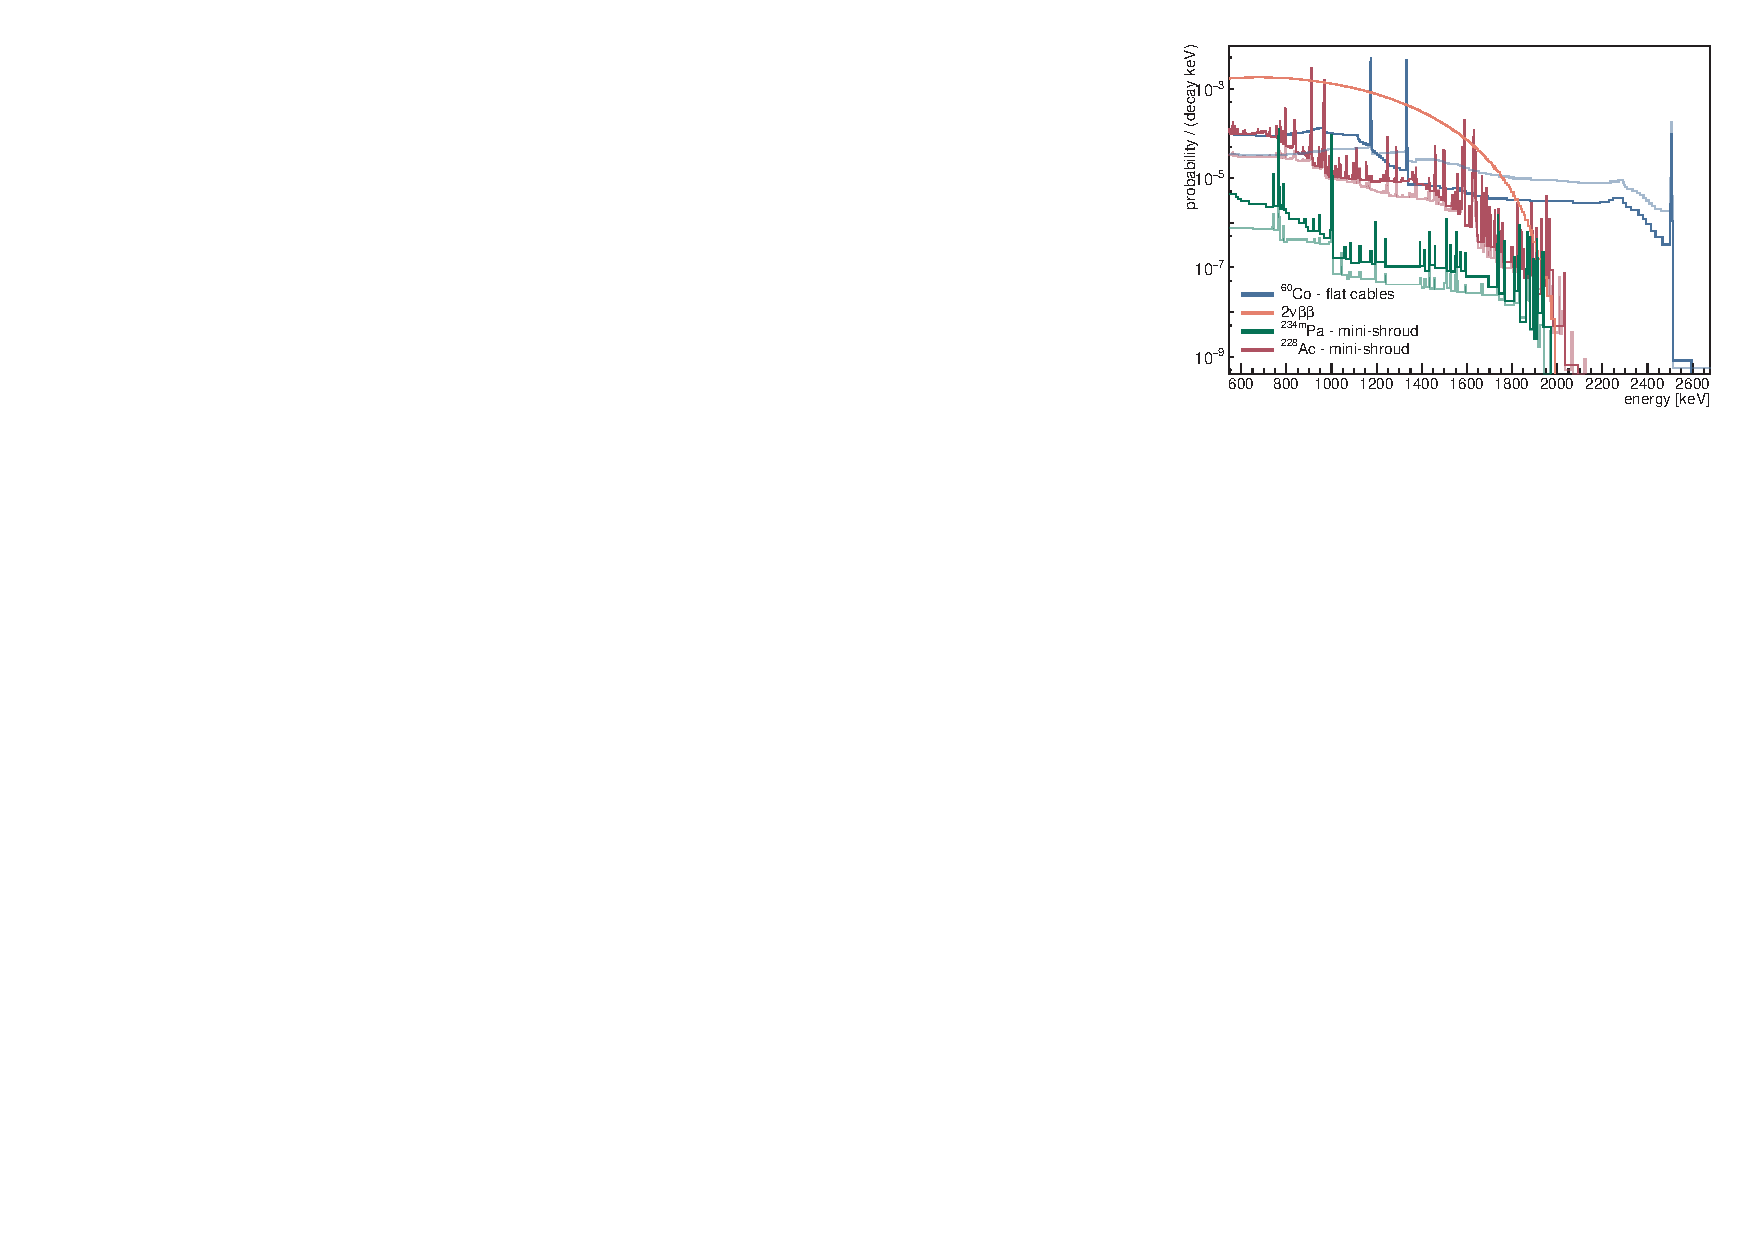
\includegraphics[width=0.48\textwidth]{plots/bkg/raw/ph2/pdfs/gmodel-pdfs-misc.pdf}}
  \hfill
  \subfloat[\label{fig:bkg:raw:ph2:pdfs:gmodel:other2}%
    \Co\ contamination in the signal and high-voltage cables and detector intrinsic
    \gesix\ \nnbb\ decay.
  ]{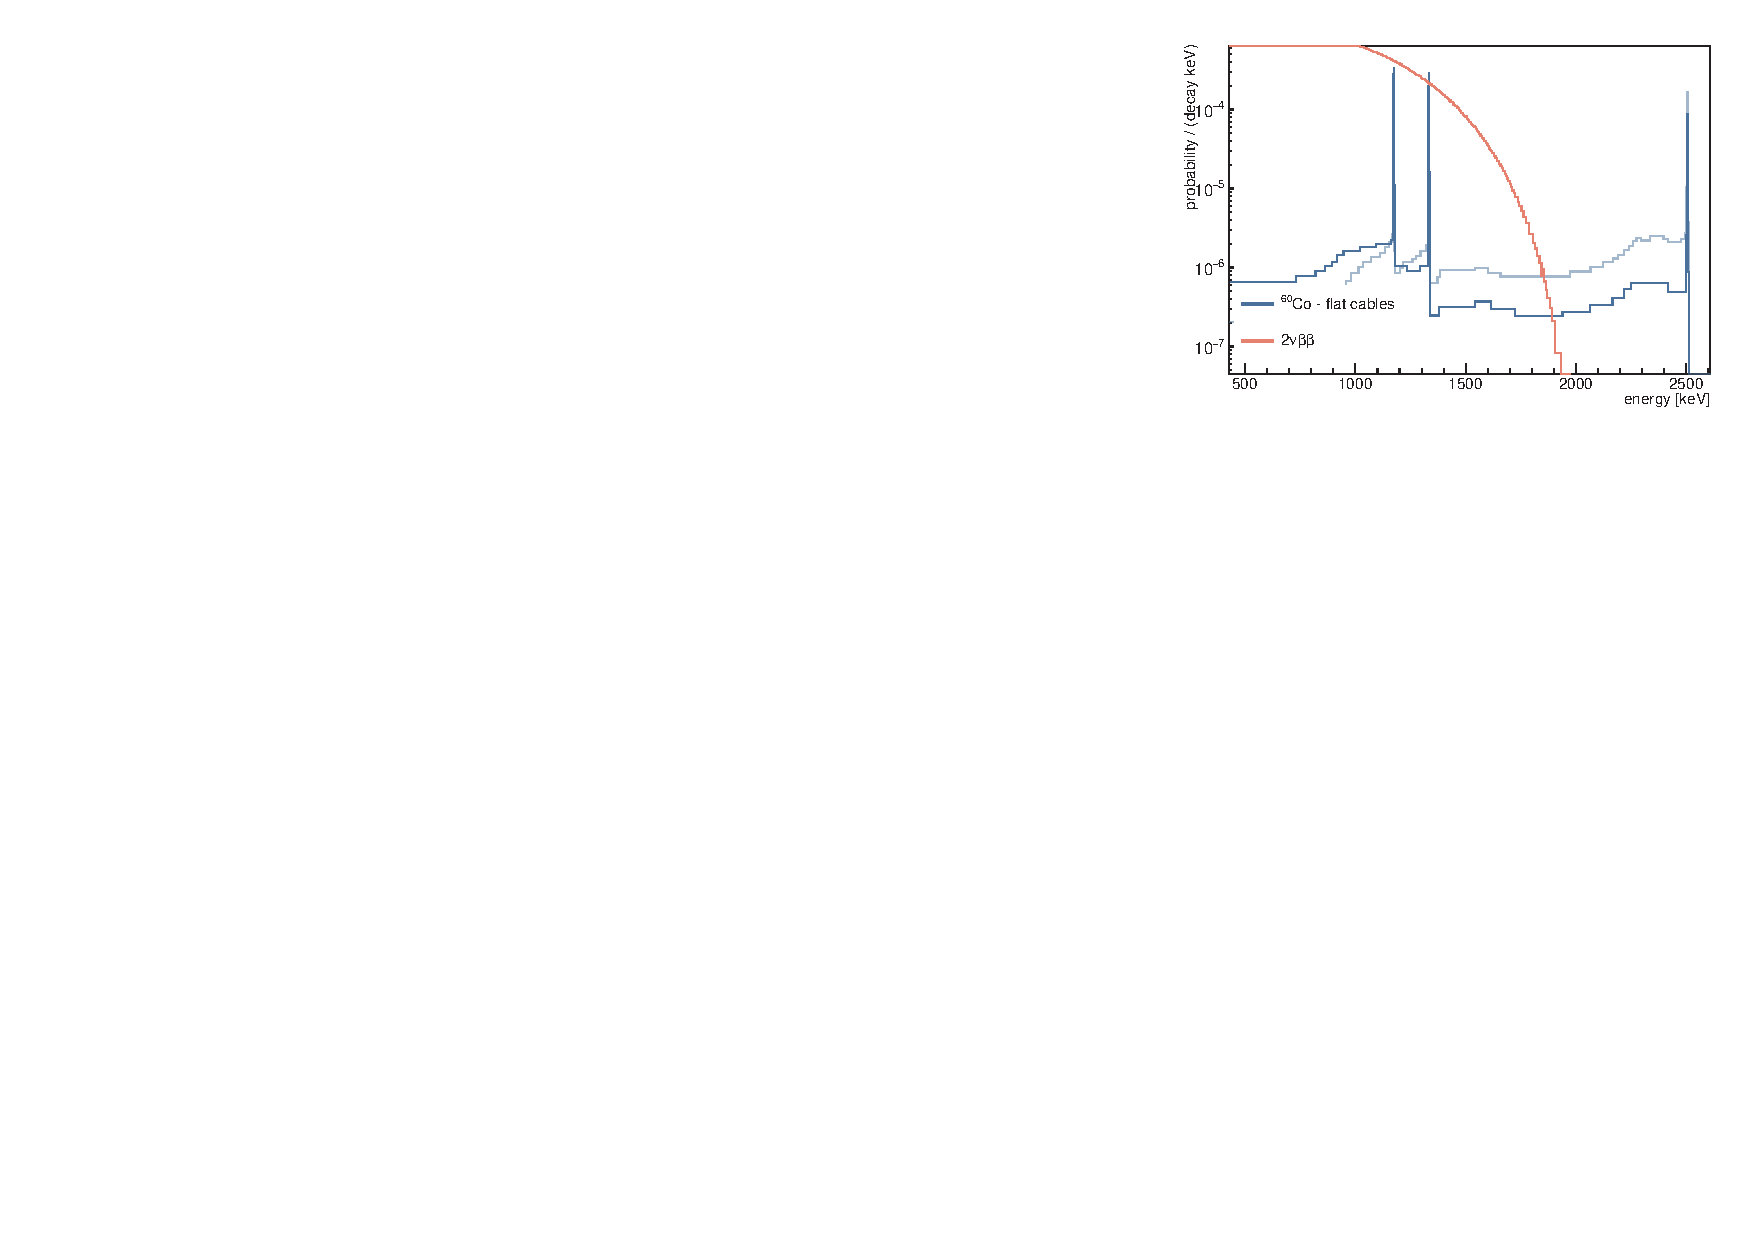
\includegraphics[width=0.48\textwidth]{plots/bkg/raw/ph2/pdfs/gmodel-pdfs-misc2.pdf}}

  \caption{%
    The pdfs for the \enrGeII\ ($\enrBEGeII + \enrCoaxII$) (in fully opaque colors) and
    the \enrGeII\ (in shaded colors) data sets in the full energy domain and relative to
    different background sources. Bayesian blocks are used to visualize histograms (see
    \cref{apdx:bayesblocks} for details. All pdfs are normalized to the number of
    simulated events.
  }\label{fig:bkg:raw:ph2:pdfs:gmodel}
\end{figure}

The structural components of the setup have been screened for their radio-purity before
deployment. Two measurement methods were used depending on the screened isotope: \g-ray
spectroscopy (Ge-\g) with High Purity Germanium (in four underground laboratories, for
details see reference~\cite{Ackermann2012}) and mass spectrometry with Inductively Coupled
Plasma Mass Spectrometers (ICP-MS)~\cite{Vacri2015}. Especially materials close to the
detectors have been screened for radioactive contaminations originating from the \Uh\ and
\Thh\ decay chains, \kvn\ and \Co. For measured activities and upper limits see
\cref{apdx:assay} and sec.~5 in~\cite{Agostini2018a}. All possible background sources
taken into consideration in this analysis are described in detail below.

\blocktitle{\Thh\ \\ \Uh}
The only isotopes simulated are \Pa, \Pbh\ and \Bih\ from the \Uh\ decay chain and \Ac,
\Bil\ and \Tl\ from the \Thh\ decay chain. The following groups of isotopes are assumed to
be in secular equilibrium:
\[
  ^{238}\text{U}  \succ ^{234\text{m}}\text{Pa}               \;\; \| \;\;
  ^{226}\text{Ra} \succ ^{214}\text{Pb} \succ ^{214}\text{Bi} \;\; \| \;\;
  ^{228}\text{Ra} \succ ^{228}\text{Ac}                       \;\; \| \;\;
  ^{228}\text{Th} \succ ^{212}\text{Bi} \succ ^{208}\text{Tl} \;.
\]
Their decay products consist of \g\  or \b\ particles with an energy higher than 520~keV
(\cref{fig:bkg:raw:ph2:pdfs:gmodel:U,fig:bkg:raw:ph2:pdfs:gmodel:Th,fig:bkg:raw:ph2:pdfs:gmodel:other}).
Less energetic particles from the remaining constituents in the chain do not enter the
energy window which is considered in the presented analysis.  The \a\ emitters from the
decay chains contaminating the thin \pplus\ electrodes are described in a separate
paragraph below.

\blocktitle{\Co}
A significant fraction of components in the \gerda\ setup is made of
copper~\cite{Agostini2018a}, which can be produced with high radio-purity but is
potentially activated by cosmic rays and contaminated by the long-lived isotope \Co\
(\cref{fig:bkg:raw:ph2:pdfs:gmodel:other}). The latter decays with a half-life of
5.2711(8)~yr; from material screening it is also expected to be found in some of the
detector high-voltage flexible flat cables.

\blocktitle{\kvn}
This isotope is found in all screened materials.  Construction materials were not
optimized for ultra-low \kvn\ content because the Q-value of its decay is well below \qbb\
and hence does not contribute to the background in the ROI. The \kvn\ decay spectrum
exhibits a \g\ line at 1460.822(6)~keV (see \cref{fig:bkg:raw:ph2:pdfs:gmodel:K40}) with
an accumulated statistics on the order of 100~cts/detector. In
\cref{fig:bkg:raw:ph2:pdfs:kmodel:K40} the expected counts per detector channel for \kvn\
simulated in different locations are shown. Using the ratio of events detected in
different detectors, information about the spatial distribution of \kvn\ can be extracted.
This spatial information is used to resolve degeneracies of \kvn\ in the energy spectra
(for details see \cref{sec:bkg:raw:ph2:kmodel}).

\blocktitle{\kvz}
A cosmogenically-produced isotope in LAr is \Arh\ ($T_{1/2} = 32.9(11)$~yr) which decays
to \kvz. The distribution of \kvz\ inside the LAr is likely to be inhomogeneous due to
drift of the ionized decay products induced by the electric field (generated by
high-voltage cables and detectors) and convection. \kvz\ decays to $^{42}$Ca via \b\ decay
with a half-life of 12.355(7)~h and a Q-value of 3525.22(18)~keV, well above \qbb (see
\cref{fig:bkg:raw:ph2:pdfs:gmodel:K42}). For the \b\ particle to be detected the decay
needs to happen within a distance of a few centimeters\footnote{The path length of \kvz\
\b\ particles in LAr is less than 1.6~cm, but bremsstrahlung photons from the interaction
with LAr can travel as far as $\sim$10~cm.} to the detector surface. As the detectors are
in direct contact with the LAr, the \b\ component of \kvz\ potentially gives one of the
most significant contributions to the background in the ROI. Therefore, we separate decays
originating inside and outside the mini-shrouds in the following analysis. The full-range
fit has little sensitivity to any potassium inhomogeneity outside the mini-shrouds. \kvz\
is hence assumed to be distributed homogeneously in this region. Based on detector-wise
observations, however, a surplus of \kvz\ above the detector array in the vicinity of the
front-end electronics is deduced (see \cref{sec:bkg:raw:ph2:kmodel}). Inside the
mini-shrouds the \b\ spectrum becomes potentially important.  Some scenarios are possible,
the closer \kvz\ decays to the detector surface, namely to the \nplus\ and \pplus\
contacts, the more \b\ particles enter the germanium. A fraction of events around \qbb\
coming from \kvz\ is potentially due to \g\ particles with higher energy and sub-percent
level branching ratio or simultaneous energy deposition of multiple \g\ particles. This
\g\ component could become important for large quantities of \kvz\ not located directly on
the detector surfaces with the \b\ particle being absorbed in the LAr. As for \kvn\ also
the \g\ line at 1525~keV of \kvz\ contains valuable information about the spatial decay
distribution of this isotope. In contrast to \kvn\ no additional information, e.g.~from
radio-purity screening measurements, is available. For more detailed information about
\kvn\ and \kvz\ see \cref{sec:bkg:raw:ph2:kmodel}.

\blocktitle{\a\ emitters}
The lithium-diffused \nplus\ detector surfaces act as a barrier for \a\ particles. The
latter can only penetrate the very thin boron-implanted \pplus-contact or the contact
separating groove. \a\ particles have to be emitted directly at the surface or from a thin
adjacent layer of LAr. Since \a\ particles have to cross the $\sim 0.5$~\mum\ thick
\pplus\ dead layer and therefore only part of their initial energy is deposited in the
active volume, this background component leads to peaks with characteristic low-energy
tails in the HPGe energy spectra (see \cref{fig:bkg:raw:ph2:pdfs:amodel}). Some \a\
events, presumably originating from the detector groove, are reconstructed with degraded
energy and lead to an additional, continuous spectral component. We find mainly \Po\ but
also traces of isotopes from the \Ra\ decay chain.

\blocktitle{detector \\ bulk \\ impurities}
Cosmogenically produced long-lived isotopes can also be found in
germanium~\cite{Meierhofer2009, Meierhofer2010, Meierhofer2012}. In particular, $^{68}$Ge
and \Co\ can occur as detector intrinsic impurities with half-lives of 270.93(13)~d and
5.2711(8)~yr.  The \bege\ detectors were kept underground during major parts of the
fabrication and characterization operations. Periods when these detectors were above
ground have been tracked in a database~\cite{Agostini2015e}.  Thus, for the well-monitored
BEGe detectors we expect impurities of 5~nuclei/kg of $^{68}$Ge and 21~nuclei/kg of \Co\
as of September 2014~\cite{Agostini2015e}. Extrapolating the expected impurities to the
whole \phasetwo\ data taking period we expect on average 0.03~cts/day from $^{68}$Ge and
0.1~cts/day due to \Co. From background modeling in Phase I~\cite{Agostini2013a} the
contribution for the coaxial detectors formerly used in the Heidelberg-Moscow
(\hdm)~\cite{Klapdor2001} and \igex~\cite{Aalseth2002} experiments is expected to be even
smaller due to their long storage underground. Simulating the expected detector bulk
impurities we find background contributions around \qbb\ of less than $10^{-4}$~\ctsper\
in both cases. Hence, we conclude that $^{68}$Ge as well as \Co\ can be neglected in the
following analysis. Potential bulk contaminations with \Uh\ and \Thh\ were studied in
reference~\cite{Agostini2016a}. Only upper limits were found, establishing germanium
crystals as material of outstanding radio-purity.  Hence, only the decay of \gesix\ via
\nnbb\ as detector intrinsic background component is considered while all other intrinsic
impurities are considered to be negligible.

\blocktitle{other \\ sources}
As discussed in reference~\cite{Agostini2013a}, prompt cosmic muon induced background
events are efficiently vetoed by the identification of \v{C}erenkov light emitted by muons
when they pass the water tank. The expected BIs, due to the direct muon and neutron fluxes
at the LNGS underground laboratory, have been estimated to be of the order
$3 \cdot 10^{-5}$~\ctsper~\cite{Freund2014} and $10^{-5}$~\ctsper~\cite{Meierhofer2012} in
earlier works, respectively.  Background contributions coming from delayed decays of
$^{77}$Ge and $^{77\text{m}}$Ge, also induced by cosmic muons, are estimated to be
$0.21 \pm 0.01$~nuclei/(kg$\cdot$yr)~\cite{Wiesinger2018} corresponding to a BI prior to the
active background suppression techniques of about $10^{-5}$~\ctsper. Also, the water tank
and LAr cryostat contaminations are expected to contribute to the \gerda\ BI with less
than $10^{-4}$~\ctsper~\cite{Ackermann2012, Barabanov2009}. All above mentioned
contributions are considered negligible in this work. Other potential sources of
background from interactions of \gesix~\cite{Meierhofer2012, Vanhoefen2018} and
$^{206}$Pb~\cite{Mei2007} with neutrons and $^{56}$Co for which no evidence was found are
not taken into consideration. The cosmogenically produced isotope \Arl\ and the
anthropogenic isotope \Kr~\cite{Winger2005}, which are dissolved in LAr, emit particles
which are dominantly less energetic than the energy window which is considered in the
presented analysis.

\section{Statistical analysis}%
\label{sec:bkg:raw:ph2:stat}

The multivariate statistical analysis, which is used to model and disentangle the
background in its components, runs on the three binned data sets \enrBEGeII, \enrCoaxII\
and \enrGeII. The single-detector data sets \enrBEGeII\ and \enrCoaxII\ contain the
reconstructed energy of all \Mone\ events whereas for the two-detector events the sum of
the two reconstructed energies is put in the \enrGeII\ data set. Moreover, the count rate
per detector is used for the two potassium \g\ lines.  The spatial event distribution is a
collection of the number of events per detector for \Mone\ events and expressed in a
matrix of pairs of detectors for all \Mtwo\ events.

\blocktitle{likelihood}
\sloppy Assuming that the number of events in each bin follows the Poisson probability
distribution $\operatorname{Poisson}(n;\nu)$, where $\nu$ is the expected mean and $n$ is the
experimentally measured number of counts, the likelihood function for a binned data set
reads $\prod_{i=1}^{N_\text{bins}} \operatorname{Poisson}(n_i;\nu_i)$. Here $\nu_i =
\sum_{k=1}^{N_\text{com}} \nu_i^{(k)}$ is the expected number of events in the $i$-th bin,
calculated as the sum of the contributions from each background component $k$;
$\nu_i(\lambda_1, \ldots, \lambda_{N_\text{com}})$ is a function of the parameters of
interests $\lambda_j$ (isotope activities, \nnbb\ half-life, etc.). The complete
likelihood function adopted for the present analysis combines the three data sets
\enrBEGeII, \enrCoaxII\ and \enrGeII:
\begin{equation}\label{eq:bkg:raw:ph2:likelihood}
  \mathcal{L}(\lambda_1, \ldots, \lambda_m \,|\, \text{data}) =
    \prod_{d=1}^{N_\text{dat}}
    \prod_{i=1}^{N_\text{bins}}
    \operatorname{Poisson}(n_{d,i};\nu_{d,i})\;.
\end{equation}

\blocktitle{statistical \\ inference}
The statistical inference is made within a Bayesian framework. Hence, to obtain posterior
probabilities for the free parameters of interest $\lambda_j$, the likelihood defined in
\cref{eq:bkg:raw:ph2:likelihood} is multiplied according to the Bayes theorem by a factor
modeling the prior knowledge of each background component as presented in
\cref{sec:bkg:raw:ph2:priors}. The computation is performed using a Markov Chain Monte
Carlo (MCMC) methods and is implemented using the BAT software package~\cite{Caldwell2008,
Beaujean2018}. Posterior probability distributions of any observable that is not a free
parameter of the likelihood function, like background index estimates, are obtained by
sampling the desired parameter from the MCMC. A \pvalue\ estimate is provided as a
goodness-of-fit measure by adopting the algorithm suggested in~\cite{Beaujean2011} for
Poisson-distributed data.  It has to be kept in mind that this \pvalue\ estimate, however,
is not as well suited for model comparison as is for instance a Bayes factor; e.g.~the
number of free parameters is not taken into account while a Bayes factor always penalizes
models that add extra complexity without being required by the data.

\blocktitle{analysis \\ window \\ and binning}
The fit range and data bins are chosen such as to exploit as much information from
spectral features as possible brought by data without introducing undesired bias. The
chosen fit range in energy space for the single-detector data sets (\enrBEGeII\ and
\enrCoaxII) starts from just above the end-point of the \Arl\ $\upbeta^-$-spectrum at
565~keV and ends just above the \Po\ peak at 5260~keV, where the event rate drops to
almost zero values. For the two-detector events (\enrGeII\ data set) the fit range starts
at 520~keV and extends up to 3500~keV. Possible additional components outside of this
range (e.g. \Arl) do neither add information to the background decomposition in the ROI
around \qbb\ nor to the analysis of \nnbb\ decay. Furthermore, at energies lower than
$\sim$100~keV the shape of the pdfs is dominated by uncertainties on the detector
transition layer model, which describes the charge-carrier collection at the interface
between the \nplus\ contact and the detector active volume. The exact nature of this
transition region is different for each detector and prone to systematic
uncertainties~\cite{Lehnert2016}.
\newpar
With an energy resolution which is typically 3--4~keV at \qbb\ (FWHM)~\cite{Agostini2018,
Agostini2019a} and better at lower energies, a fixed bin size of 1~keV was chosen for all
data sets. The only exceptions are the two \g\ lines from \kvn\ and \kvz\ each of which is
combined in a single bin from 1455~keV to 1465~keV and from 1520~keV to 1530~keV,
respectively. This is done in order to suppress any systematic uncertainties of the energy
calibration and resolution model that affect the position and shape of the \g\
lines~\cite{Agostini2019}.

\blocktitle{likelihood \\ factorization}
A feature of the selected data is that the likelihood in
\cref{eq:bkg:raw:ph2:likelihood} can be factorized in uncorrelated parts which can be
studied individually and in detail. In the following we shortly outline the parts of the
data which were studied in depth based on the approach of factorizing the likelihood into
uncorrelated parts. Finally, the results of these analyses are incorporated into a
full-range fit. This procedure is equivalent to a simultaneous analysis of all data but
increases the input knowledge for the fit and breaks down the computational complexity in
smaller steps.

\blocktitle{potassium \\ tracking \\ analysis}
As can be noted from \cref{fig:bkg:raw:ph2:pdfs:gmodel:K40} and
\cref{fig:bkg:raw:ph2:pdfs:gmodel:K42} the pdfs of \kvn\ and \kvz\ in energy from
different locations are prone to degeneracies and hence parameter correlation. Their most
prominent \g\ lines at 1461~and 1525~keV, respectively, contain information on the spatial
distribution while the two-detector events contain information about the angular
distribution of Compton scattered events. Their combination is beneficial in order to pin
down the potential location of the two potassium isotopes. In total the \Mone\ data
contains 4472~cts in $1461 \pm 4$~keV and 6718~cts in $1525 \pm 4$~keV while the \Mtwo\
events contain 554~cts in $1461 \pm 6$~keV and 865~cts in $1525 \pm 6$~keV, respectively.
An analysis of the number of events in the two potassium \g\ lines in each detector (and
detector pair) is used to exploit mainly top-down and rotational asymmetries in the \kvn\
and \kvz\ distributions. The events in the two energy windows are classified according to
the detectors in which an energy deposition was registered, so to exploit the available
information about the event location. In the following this classification procedure will
be referred to as \textit{projection in detector space}. The treatment of the likelihood
in \cref{eq:bkg:raw:ph2:likelihood} is outlined in detail in
\cref{sec:bkg:raw:ph2:kmodel}.  The number of events in all other \g\ lines is too low in
order to adopt a useful detector-wise analysis. The spatial analysis of \kvn\ and \kvz\ is
incorporated in the full-range fit by directly employing the posterior parameter
distributions as prior information.\footnote{By adopting this approach, a part of the data
in the potassium \g\ lines region is analyzed twice: first in the potassium-tracking
analysis and then in the full-range fit. Nevertheless, considering that the two analyses
exploit different data features (i.e.~count rate per detector and total count rate per
energy) and the overlap between the two data set is minimal, the overall effect is
negligible.}

\blocktitle{\a\ events background analysis}
The single-detector energy spectra above 3.5~MeV (the Q-value of \kvz\ \b\ decay) are
strongly dominated by \a\ events. They are not present in two-detector data due to the
short range of \a\ particles in LAr and germanium. Also, this component is not correlated
to other backgrounds considered here because it peaks at energies well above the highest
\g\ emission energies and \b\ decay Q-values. A careful study was carried out considering
various \pplus\ contact thickness and event rates to reproduce the \Po\ peak. In order to
reproduce \a\ events with degraded energy an empirical model is fit to the data. A linear
function with free slope and offset and a cut-off below the maximum of the \Po\ peak fits
the data well. The agreement of the \a\ background model with the data is demonstrated in
\cref{sec:bkg:raw:ph2:amodel} and \cref{apdx:timealpha}. Information from the detailed
analysis of the high-energy \a\ region is incorporated in the full-range fit using a
combined pdf that summarizes the \Po\ peak plus the \Ra\ decay chain and a linear floating
component for energy-degraded \a\ events.

\blocktitle{prior \\ distributions}
The following criteria are adopted to convert the prior information described in
\cref{sec:bkg:raw:ph2:priors} into prior probability distributions on the parameters of
interest to be used in Bayesian inference: if a measured value with uncertainty is
available for a background contamination then a Gaussian distribution with a corresponding
centroid and a $1\sigma$ width is adopted. In presence of a 90\% C.L.~upper limit,
instead, an exponential prior distribution is constructed with 90\% of its area covering
parameter values from 0 up to the given 90\% C.L.~upper limit. A uniform prior
distribution is assigned to components for which no measured value or upper limit is
available. Ranges for uniform priors are initially taken very wide, in order to span a
large portion of the allowed parameter space, then optimized to contain at least 99\% of
the posterior distribution. As mentioned before, in addition to the information from
screening measurements, prior distributions for \kvn\ and \kvz\ are constructed
considering the posterior inference from their spatial distribution. Moreover, as \Bih\ is
part of the \Ra\ decay chain, we constrain a \Bih\ component on the \pplus\ contact by a
Gaussian prior extracted from the obtained \Ra\ activity based on the energy estimator in
the high-energy \a\ region.

\section{\texorpdfstring{\a\ events analysis}{alpha events analysis}}%
\label{sec:bkg:raw:ph2:amodel}

Above an energy of 3.5~MeV almost all registered events are due to \a-emitting isotopes.
The respective part of the full likelihood can be approximately factorized and studied
separately. \a\ particles have a very short range in LAr as well as in
germanium\footnote{In the continuous slowing down approximation (CSDA) the range of \a\
particles is estimated to be of 50~\mum\ and 20~\mum\ for LAr and germanium,
respectively~\cite{Berger2017}.} and are able to reach a detector's active volume only
through the very thin (of the order of 500~nm) \pplus\ contact surface. Therefore, the \a\
emitter contamination is detector-specific and depends only on the \pplus\ surface
contaminations. For this reason, \enrBEGeII\ and \enrCoaxII\ detector data above 3.5~MeV
is analyzed independently. The projection in detector space shows no significant correlation
between events in different detectors and hence contains no further useful information.
Additionally, the number of events in a single detector is not sufficient to further split
the data on a detector-by-detector basis. The two data sets are uncorrelated and the
statistical analysis can be carried out for each \Mone\ data set separately. As already
mentioned, \a\ events in the \Mtwo\ data are not observed due to the short range of these
particles.

\blocktitle{sources}
All contaminations found are constituents of the \Uh\ decay chain. The main surface
contamination observed is \Po\ which occurs either as an incident contamination and decays
in time with a half-life of $138.3763(17)$~days~\cite{Be2008} or is fed by a \Pbl\ contamination
with a stable rate in time. The spectral form is identical for both cases and
can only be disentangled by analyzing the \a\ event rate in time.
Above the \Po\ peak very few events are observed. In the \enrBEGeII\ data set we find only
four events with an energy larger than 5.3~MeV, while in the \enrCoaxII\ data set 22 such
events are observed, 14 of which in a single detector \ANG{2}
(see~\cref{tab:bkg:raw:ph2:amodel:rncts}). These events are due to \a\ decays from \Rn\
and subsequent isotopes on the \pplus\ detector surfaces. \ANG{2} also shows a higher \Ra\
(mother nucleus of \Rn) contamination which suggests dominantly a surface contamination
with \Ra\ rather than \Rn\ dissolved in LAr. In the latter case the decay chain would
be broken, as only the gaseous \Rn\ can emanate from the construction materials.
Unfortunately, the number of counts is too low to distinguish the spectral shape above
5.3~MeV and disentangle a surface contamination with \Ra\ from \Rn\ dissolved in LAr. A
comparison between the counts observed above 5.3~Mev and the \Bih\ 609~keV \g\ line
suggests that \a\ events due to a dissolved \Rn\ contamination would not produce
observable counts in said energy region. Assuming that all \Bih\ observed comes from
dissolved \Rn\ leads, in fact, to a specific activity smaller than 10~\mubq/kg. Hence, in
the following, we will only consider a \pplus\ surface contamination with \Ra\ and all
subsequent isotopes to which we refer as the \Ra\ decay chain. The \Po\ and \Ra\
contaminations are not necessarily spatially correlated.
\begin{table}
  \centering
  \caption{%
    Observed number of counts with energy >5.3~MeV belonging to
    the \Ra\ decay chain. Detectors with zero counts are not listed.
  }\label{tab:bkg:raw:ph2:amodel:rncts}
  \begin{tabular}{cccc}
    \toprule
    data set                    & detector & channel & \Ra\ chain [cts] \\
    \midrule
    \multirow{3}{*}{\enrBEGeII} & \GD{61C} & 16      & 1                \\
                                & \GD{79B} & 32      & 1                \\
                                & \GD{89A} & 35      & 2                \\
    \midrule
    \multirow{6}{*}{\enrCoaxII} & \ANG{1}  & 36      & 2                \\
                                & \ANG{2}  & 27      & 14               \\
                                & \ANG{3}  & 10      & 1                \\
                                & \ANG{4}  & 29      & 1                \\
                                & \ANG{5}  &  8      & 2                \\
                                & \RG{1}   &  9      & 2                \\
    \bottomrule
  \end{tabular}
\end{table}

\blocktitle{model}
Due to the very short range of \a\ particles the energy spectrum of \a\ decays exhibits a
line with a pronounced low-energy tail. The tail is formed when the decay occurs under an
incident angle with respect to the contact and the \a\ particle loses part of its energy
before reaching the detectors active volume. The maximum is shifted with respect to the
full emission energy which is due to energy loss inside the electrode and depends on its
minimal thickness. The detectors have slightly different contact thicknesses, and the
\pplus\ contact of a single detector may also be intrinsically inhomogeneous.  Therefore,
the \Po\ peak is modeled with a mixture of pdfs obtained from simulations with different
contact thicknesses, shown in \cref{fig:bkg:raw:ph2:pdfs:amodel}. Due to the low number of
counts observed in the \Ra\ chain it is sufficient to model this component with only one
pdf. Furthermore, the isotope contamination is assumed to halve at each decay step. A
reduction effect of the subsequent \a\ decays in the \Rn\ chain had been observed in
\phaseone\ and attributed to possible recoil off the surface into the
LAr~\cite{Agostini2013}. We adopt this explanation in our model although we note that the
number of events observed with an energy >5.3~MeV is not sufficient to confirm such an
effect.
\newpar
Dedicated measurements~\cite{Agostini2013b} have shown that events originating in the
contact separating groove are partly reconstructed with degraded energy. A
simulation-based model of these energy-degraded events is not available yet. We
approximate this component with an empirical linear distribution truncated below the
maximum of the \Po\ peak. Such a component accommodates also eventual \a\ decays in the
LAr in very close vicinity to the \pplus\ detector surface. However, the number of events
found with an energy >5.3~MeV is too low to fully account for the linearly modeled
distribution.

\begin{figure}
  \centering
  \subfloat[%
    \Po\ \a\ decays on \pplus\ contact surface for different thicknesses of the inactive
    contact layer. For 0~nm the nuclear recoil energy can be absorbed and some energy can
    be lost in the LAr.\label{fig:bkg:raw:ph2:pdfs:amodel:Po}%
  ]{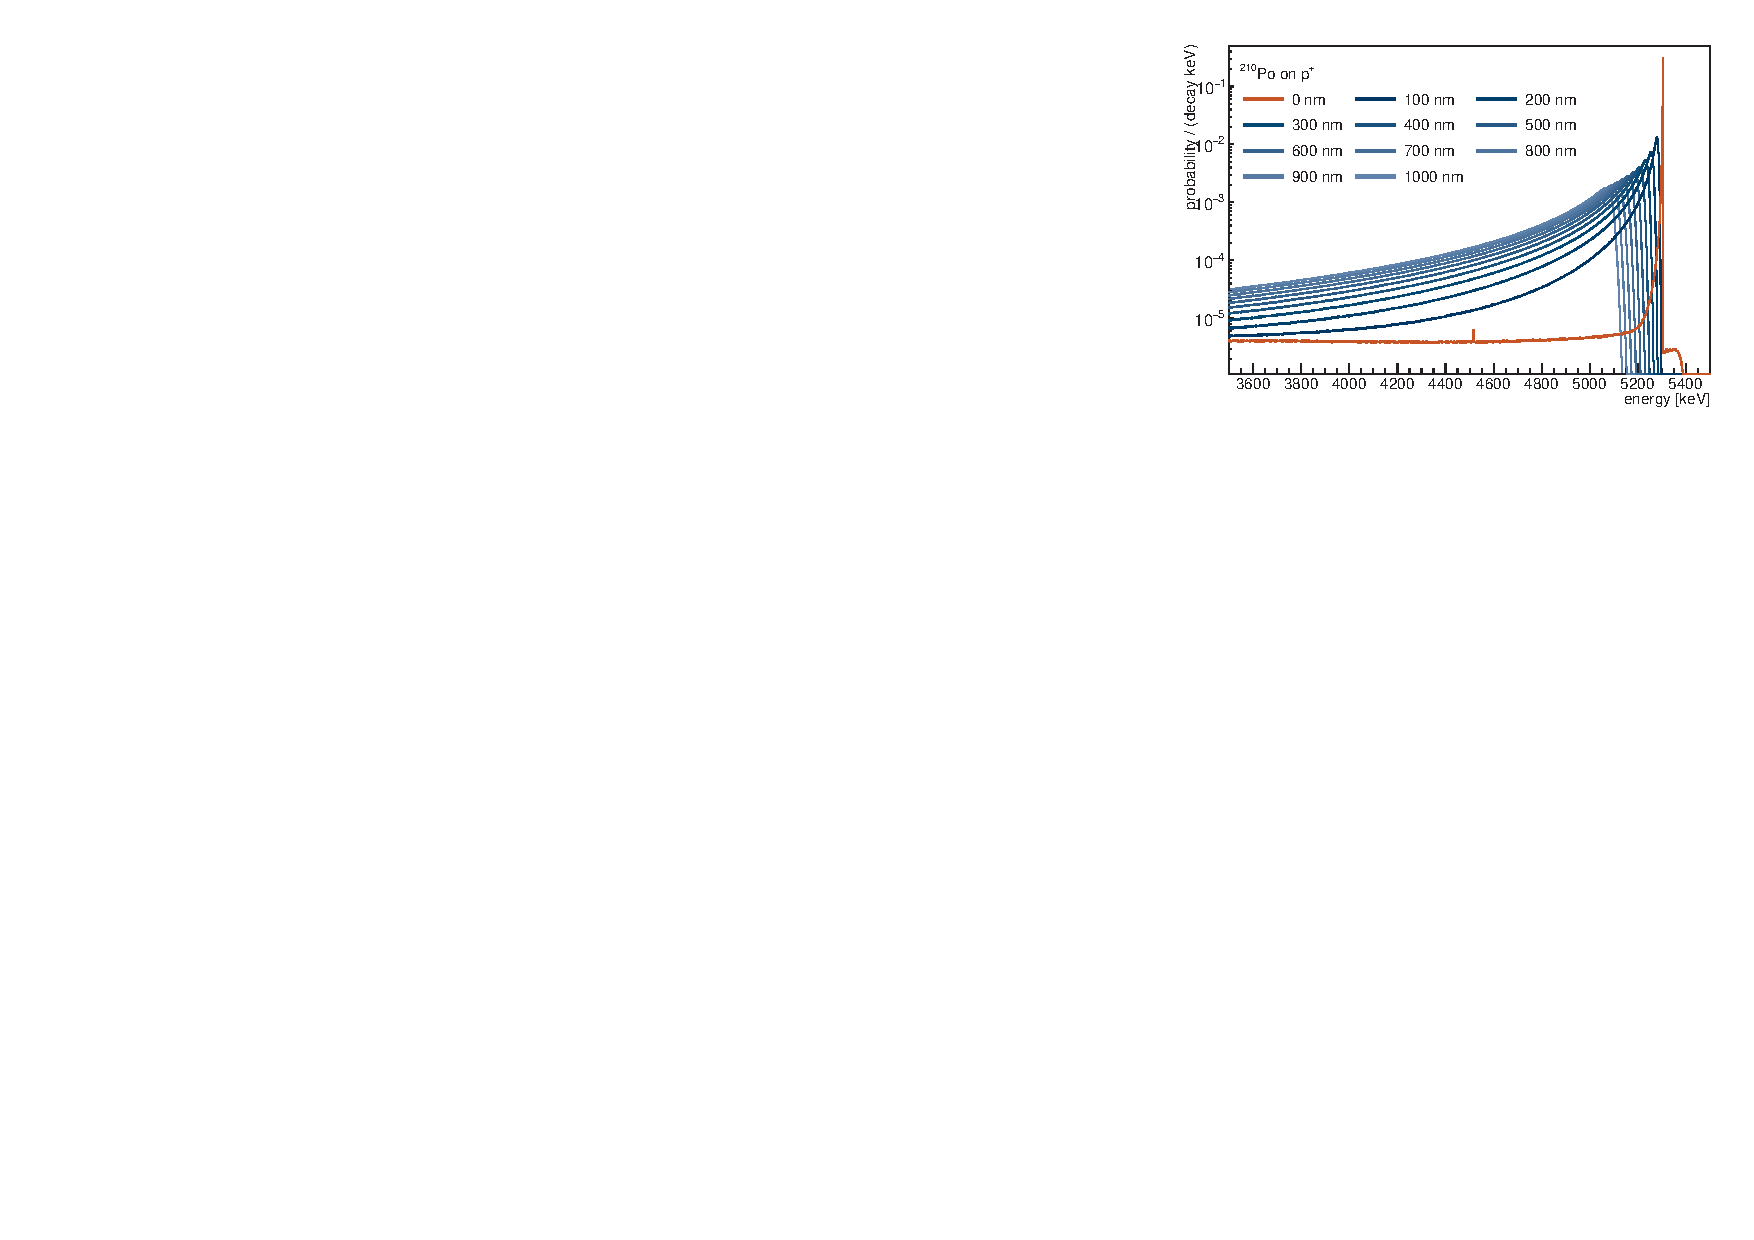
\includegraphics[width=0.48\textwidth]{plots/bkg/raw/ph2/pdfs/amodel-pdfs-Po210.pdf}}
  \hfill
  \subfloat[%
    \a\ decays from the \Ra\ decay sub-chain (\Ra, \Rn, $^{218}$Po and $^{214}$Po) on the
    detectors \pplus\ contact surface for different depths of the inactive contact layer.
    The isotope contamination is assumed to halve at each decay step, because of the
    recoil of the nuclei in LAr.\label{fig:bkg:raw:ph2:pdfs:amodel:Ra}%
  ]{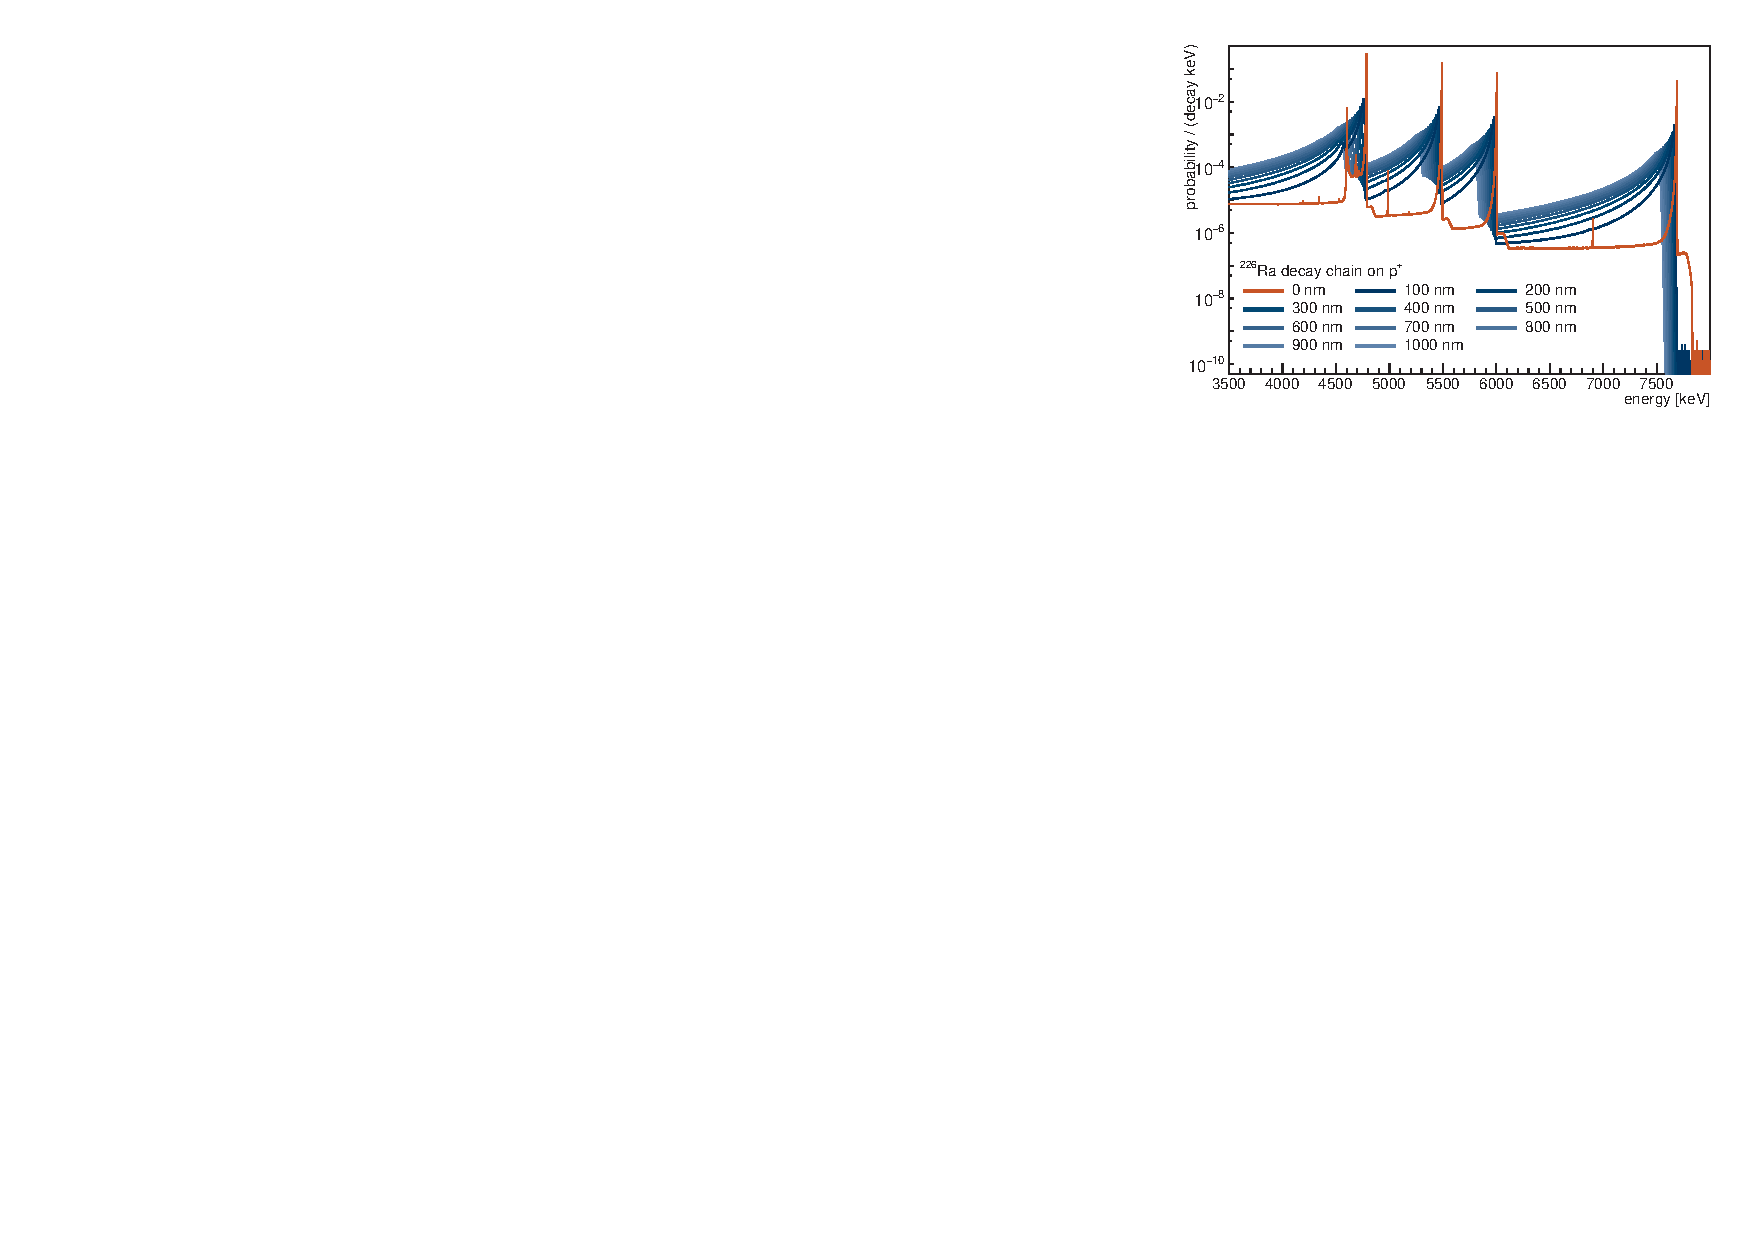
\includegraphics[width=0.48\textwidth]{plots/bkg/raw/ph2/pdfs/amodel-pdfs-U.pdf}}
  \caption{}%
  \label{fig:bkg:raw:ph2:pdfs:amodel}
\end{figure}

\blocktitle{analysis}
The likelihood function for modeling the high-energy region dominated by \a\ decays runs
only on single-detector data, namely \enrBEGeII\ and \enrCoaxII\ separately, in a range
from 3.5~MeV to 5.25~MeV. Events with an energy higher than 5.25~MeV are put in a single
overflow bin:
\begin{equation}
  \mathcal{L}_{\alpha}{(\lambda_1,\ldots,\lambda_m\,|\,n)} =
  \prod_{i=1}^{N_\text{bins}} \operatorname{Poisson}(n_{i};\nu_{i})\;
  \label{eq:bkg:raw:ph2:amodel:likelihood}
\end{equation}
A flat prior probability is assigned to each of the fit parameters $\lambda_i$. Both data
sets are fit separately with a fixed bin size of 10~keV\footnote{The calibration curves
are accurate on the sub-keV level up to the highest \g\ energy of about 2.6~MeV emitted
by the \Th\ calibration sources. Although no major non-linearity effects were found the
same accuracy cannot be guaranteed at 6~MeV. Deviations from linearity at this energy are
within 10~keV, hence, we increase the bin size in the higher energy range.} as the \a\
contamination is detector individual and the two single-detector data sets are
uncorrelated in the respective energy window.
\newpar
The fit results are shown in \cref{fig:bkg:raw:ph2:amodel:resultsplot} and listed in
\cref{tab:bkg:raw:ph2:amodel:results}. The \Po\ component is modeled with a combination of
\pplus\ contact thicknesses from 400 to 600~nm for the \enrBEGeII\ data set and from 300
to 700~nm for the \enrCoaxII\ data set in steps of 100~nm. Further \Po\ components are
rejected by a Bayes factor analysis.  Impurities belonging to the \Ra\ chain are mostly
located on \ANG{2} and thus a fit of the \enrCoaxII\ data set using a single \pplus\
thickness describes this component well. For the \enrBEGeII\ data set we observe a very
small number of counts for the \Ra\ chain, therefore, also in this case a single component
is sufficient. We determine a best-fit value of 100~nm and 500~nm, respectively. The
estimated \pvalue\ for \enrBEGeII\ is 0.2 whereas the \pvalue\ for \enrCoaxII\ is 0.3. The
dominant spectral component below 4.5~MeV is due to degraded \a\ events which extends down
to the ROI.

\begin{figure}
  \centering
  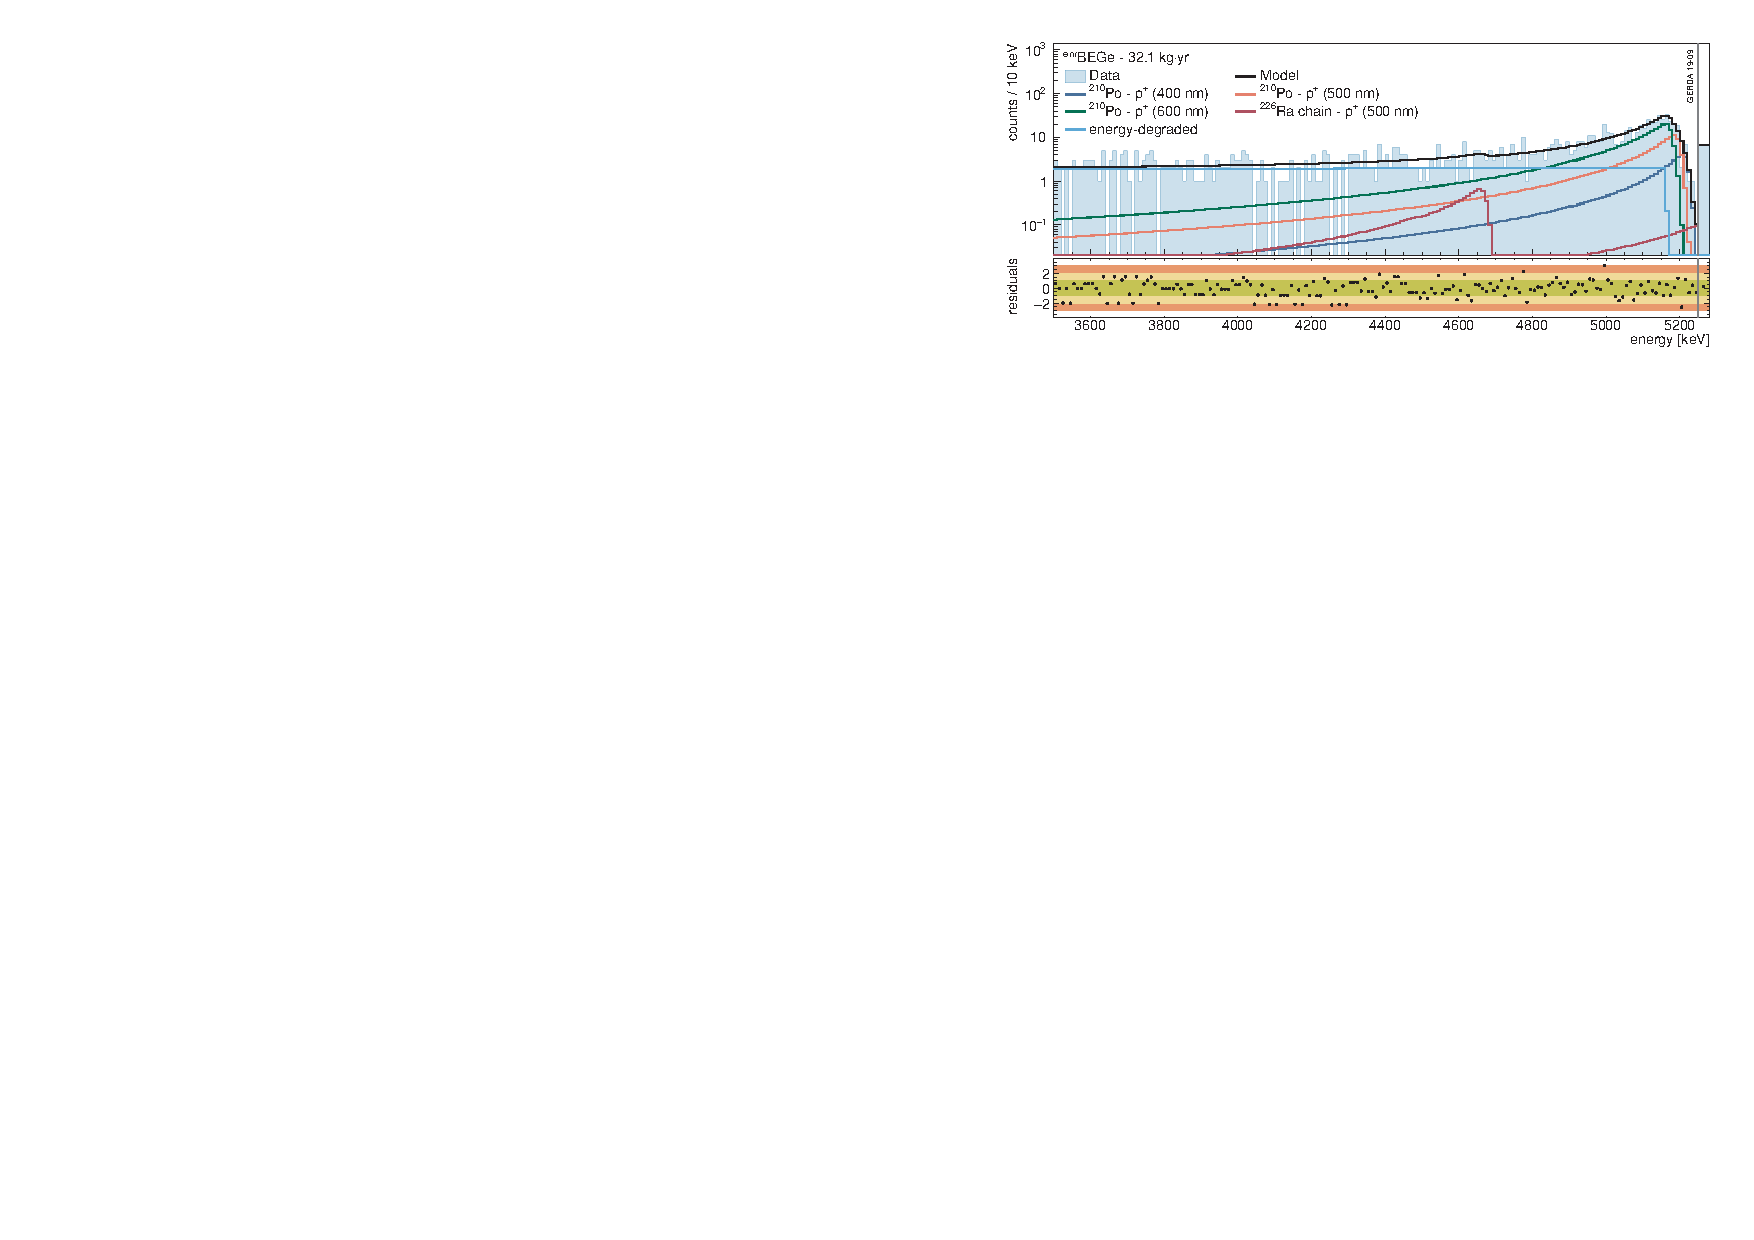
\includegraphics{plots/bkg/raw/ph2/results/amodel/amodel-enrBEGe.pdf}
  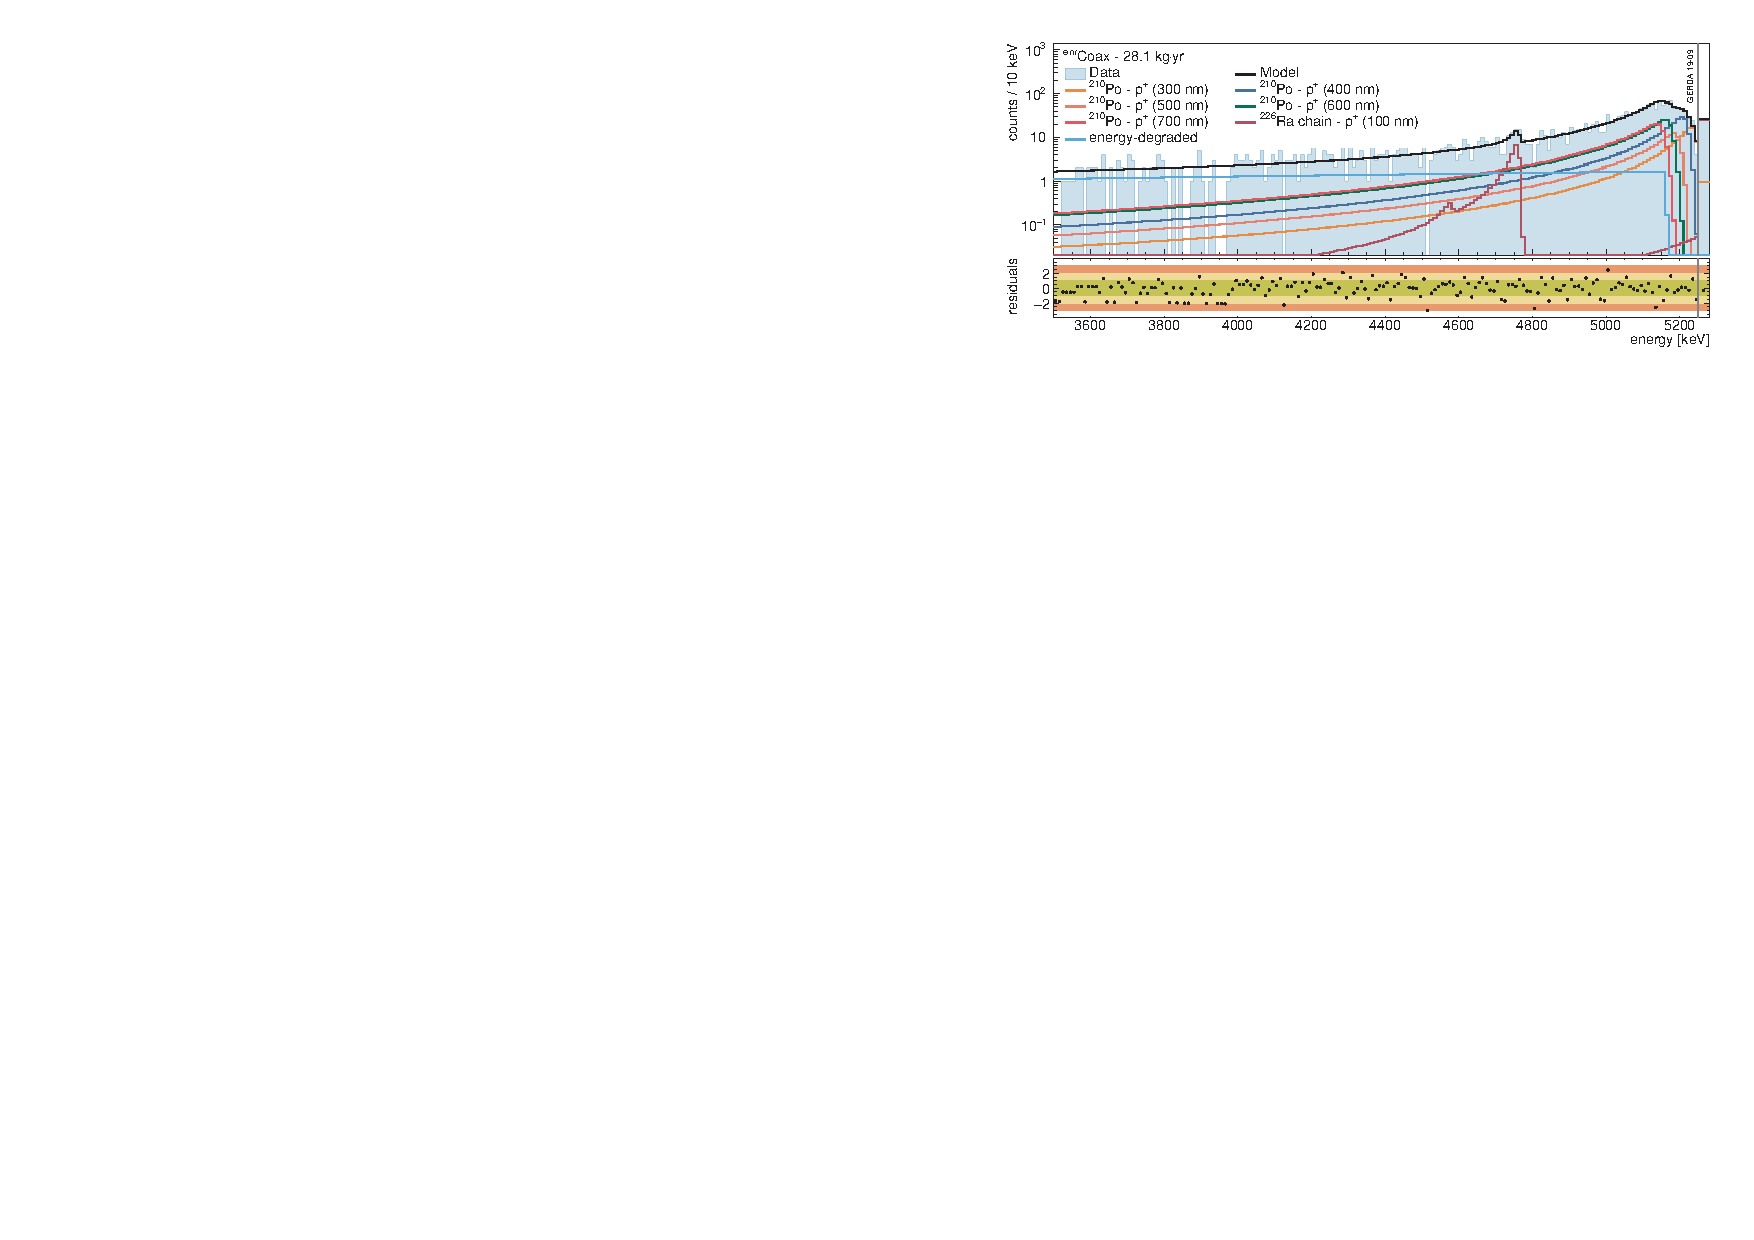
\includegraphics{plots/bkg/raw/ph2/results/amodel/amodel-enrCoax.pdf}
  \caption{%
    Fit results of the \a\ events background analysis for \enrBEGeII\
    (top) and \enrCoaxII\ (bottom). The last bin contains all events above
    5250~keV.
  }\label{fig:bkg:raw:ph2:amodel:resultsplot}
\end{figure}

\begin{table}
\centering
  \caption{%
    Fit results of the \a\ events background analysis for the
    \enrBEGeII\ and \enrCoaxII\ data sets. Values are given in counts in the
    full pdf range from 40~keV to 8000~keV.
  }\label{tab:bkg:raw:ph2:amodel:results}
  \begin{tabular}{rlccr@{ }l}
  \toprule
  \mr{2}{data set}   & \mr{2}{component} & contact & global mode & \mc{2}{marg.~mode}      \\
                     &                   & [nm]    & [cts]       & \mc{2}{68\% C.I.~[cts]} \\
  \midrule
  \mr{6}{\enrBEGeII} & \mr{4}{\Po}       & 400     & 49          & 50   & $[34,76]$        \\
                     &                   & 500     & 162         & 165  & $[107,222]$      \\
                     &                   & 600     & 346         & 342  & $[278,391]$      \\
                     &                   & comb.   & --          & 555  & $[523,586]$      \\
                     & \Ra\ chain        & 500     & 20          & 20   & $[15,29]$        \\
                     & energy-degraded   & --      & --          & 845  & $[698,948]$      \\
  \midrule
  \mr{8}{\enrCoaxII} & \mr{6}{\Po}       & 300     & 167         & 165  & $[140,208]$      \\
                     &                   & 400     & 363         & 368  & $[272,430]$      \\
                     &                   & 500     & 182         & 175  & $[83,338]$       \\
                     &                   & 600     & 433         & 420  & $[233,582]$      \\
                     &                   & 700     & 404         & 410  & $[295,537]$      \\
                     &                   & comb.   & --          & 1555 & $[1511,1609]$    \\
                     & \Ra\ chain        & 100     & 58          & 59   & $[49,70]$        \\
                     & energy-degraded   & --      & --          & 485  & $[426,599]$      \\
  \bottomrule
\end{tabular}

% vim: nowrap

\end{table}

\fillme{mention to time alpha}

\section{Potassium-tracking analysis}%
\label{sec:bkg:raw:ph2:kmodel}

The two full-energy lines of \kvn\ and \kvz\ at 1461~keV and 1525~keV are distinct
features of the energy spectrum shown in \cref{fig:bkg:raw:ph2:datasets}. Being a relevant
source of background for double-beta decay, the two potassium isotopes play a crucial role
in the background modeling process in \gerda. Uncertainties in their origin and
distribution propagate directly to searches for exotic physics like Majorons, Lorentz
invariance-violating processes or decay modes to excited states of \nnbb\ decay in which
the shape of the \nnbb\ decay spectrum is a unique feature and thus need to be well
understood. In the following the focus will be on the characteristics of the events
constituting these two intense \g\ lines. In order to extract information about the
spatial distribution of \kvn\ and \kvz\ contamination around the \gerda\ array, a
treatment on a detector-by-detector basis is advantageous. The two \g\ lines contain
enough statistics for such an analysis to be meaningful and constitute samples with a high
signal to background ratio.

\blocktitle{sources}
Initial observations in \phasetwo\ have shown that the \kvn\ and \kvz\ full-energy line
intensities have increased by a factor of 4 and 2, respectively, in the single-detector
data compared to \phaseone~\cite{DAndrea2017}. The \kvz\ increase in activity can be
attributed to the exchange of the mini-shrouds material from copper to nylon\footnote{The
exchange of material from copper to nylon was necessary in order to properly propagate the
LAr scintillation light which otherwise would be blocked.} during the \phasetwo\ upgrade:
The electric field generated by the detectors bias high voltage is not screened by the
conductive material anymore. The \kvz\ ions can be attracted from a larger LAr volume into
the vicinity of the detectors.  Moreover, the unshielded high-voltage cables could be an
explanation for the higher rate of \kvz\ events seen in the uppermost detectors in the
\gerda\ array. The higher \kvn\ event rate, on the other hand, is possibly attributable to
the glue used for the nylon mini-shrouds and other new materials introduced with the LAr
veto system. The exact amount, location and radio-purity of the glue is not precisely
known.  All changes to the setup that have been made during the upgrade to \phasetwo\ are
described and motivated in exhaustive detail in reference~\cite{Agostini2018a}.

\blocktitle{data set}
Data in two energy windows around the potassium \g\ lines is projected in detector index
space, such that, for single-detector data, each data point $n_i$ represents the total
counts in detector $i$ in the respective window. For two-detector data the detector space
is two-dimensional, and each data point $n_{ij}$ represents the number of events for which
energy is deposited in detector $i$ and detector $j$.  The events in the potassium lines
(denoted with \m{K40} and \m{K42} in the following) are selected in a $\pm 3\sigma$ energy
interval around the respective line, rounded up to an integer number of keV to match the
specific energy windows in the energy distributions with 1~keV binning.  $\sigma$ is the
energy resolution in the respective energy window.  Additionally, three side-bands
(\m{SB1}, \m{SB2} and \m{SB3} in the following) are used to estimate the continuum below
and above the \g\ lines. Considering the further subdivision in single- (\m{M1-}) and
two-detector (\m{M2-}) data, this leads to the definition of $5 \times 2$ energy regions,
summarized in~\cref{tab:bkg:raw:ph2:kmodel:regions-cts}. A visual representation of the
selected windows can be found in~\cref{fig:bkg:raw:ph2:kmodel:regions}. Pdfs for \Bih\ on
the flat cables and detector intrinsic \nnbb\ decays are used to estimate the background.
Other components are expected to contribute less in the respective energy windows.

\begin{table}
  \centering
  \caption{%
    Energy ranges and corresponding number of events for the potassium-tracking analysis
    (visualized in \cref{fig:bkg:raw:ph2:kmodel:regions}). Note that the windows for
    two-detector data are larger as the two single-detector energy resolutions are folded
    in the summed energy spectrum.
  }\label{tab:bkg:raw:ph2:kmodel:regions-cts}
  \begin{tabular}{ccccc}
    \toprule
             & \Mone\ [keV]  & cts. & \Mtwo\ [keV]  & cts. \\
    \midrule
    \m{K40}  & $[1457,1465]$ & 4472 & $[1455,1467]$ & 554  \\
    \m{K42}  & $[1521,1529]$ & 6718 & $[1519,1531]$ & 865  \\
    \midrule
    \m{SB1}  & $[1405,1450]$ & 1852 & $[1405,1450]$ & 452  \\
    \m{SB2}  & $[1470,1515]$ & 1124 & $[1470,1515]$ & 326  \\
    \m{SB3}  & $[1535,1580]$ & 533  & $[1535,1580]$ & 41   \\
    \bottomrule
  \end{tabular}
\end{table}

\begin{figure}
  \centering
  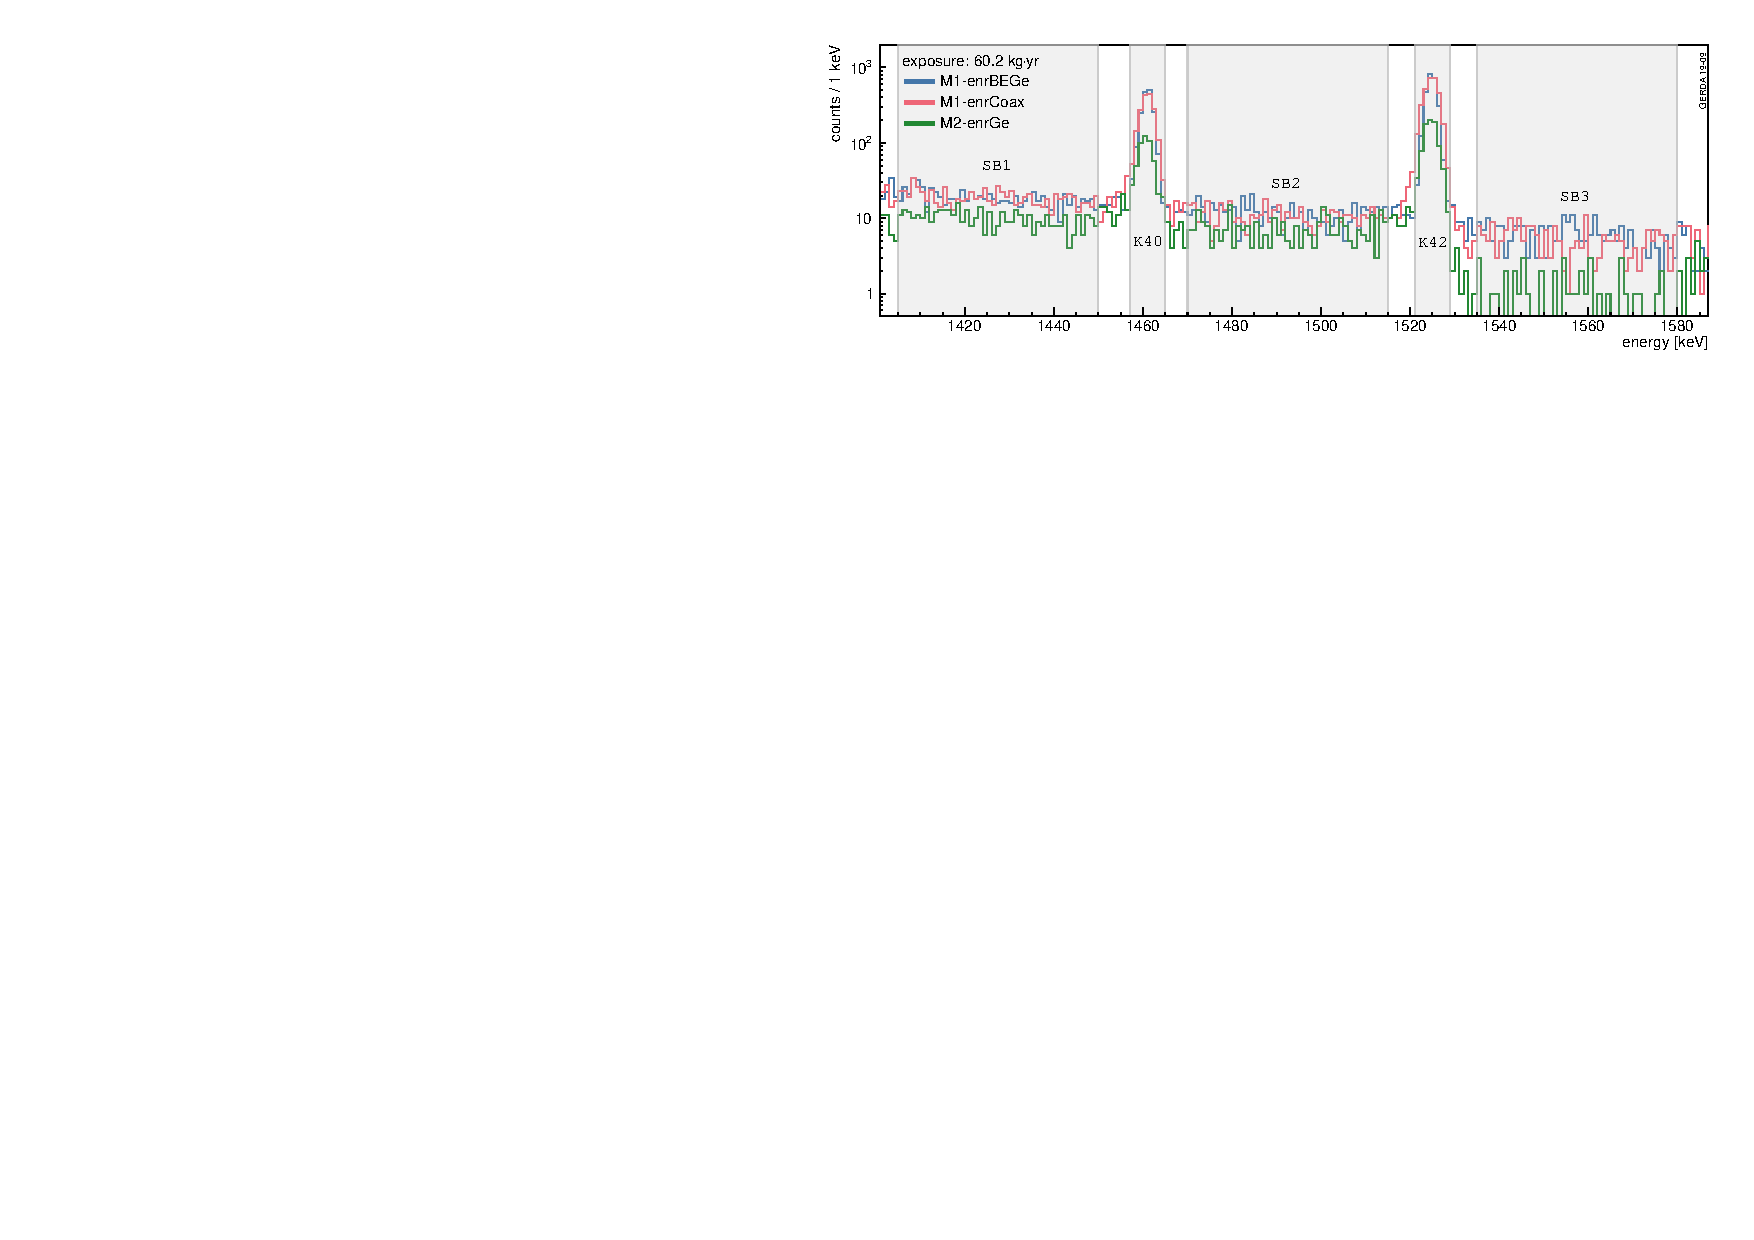
\includegraphics[width=0.8\linewidth]{plots/bkg/raw/ph2/kmodel-regions.pdf}
  \caption{%
    Visual representation of the five energy ranges defined for the potassium-tracking
    analysis. The exact intervals and counts are given in
    \cref{tab:bkg:raw:ph2:kmodel:regions-cts}.
  }\label{fig:bkg:raw:ph2:kmodel:regions}
\end{figure}

\blocktitle{likelihood}
The statistical approach of factorizing the likelihood is described in
\cref{sec:bkg:raw:ph2:stat}. The part of the likelihood analyzed here runs simultaneously
on the $5 \times 2$ energy ranges presented above. Following the previously introduced
naming convention introduced it reads:
\begin{equation}\label{eq:bkg:raw:ph2:kmodel:likelihood}
  \mathcal{L}_\text{K}(\lambda_1,\ldots,\lambda_{m'}\,|\,n) =
  \prod_{d=1}^{N_\text{dat}}
  \left\{
    \prod_{i=1}^{N_\text{det}}
    \operatorname{Poisson}(n_{d,i}^\text{\m{M1}};\nu_{d,i}^\text{\m{M1}})
    \times
    \prod_{j<k}^{N_\text{det}}
    \operatorname{Poisson}(n_{d,jk}^\text{\m{M2}};\nu_{d,jk}^\text{\m{M2}})
  \right\}\;,
\end{equation}
where the index $i$ runs over the bins (i.e.~detectors) and the index $d$ over the 5
considered energy windows, namely the three side-bands \m{SB1}, \m{SB2}, \m{SB3} and the
two line-bands \m{K40} and \m{K42}.  The \m{M2-} data sets are two-dimensional in detector
space and run over the two indices $j$ and $k$.

\blocktitle{priors}
Gaussian prior probability distributions for the \kvn\ activity are built from
radio-purity screening measurements (see \cref{apdx:assay}). For \kvz, for which no
screening information is available, uniform priors are adopted, with the exception of the
two \kvz\ components located on the \nplus\ contact surface of \bege\ and \scoax\
detectors. \kvz\ can be attracted to the \nplus\ surface by the electrical field created
by the high voltage potential applied to the detectors. Both components are expected to be
correlated by the volume ratio of the mini-shrouds (3:2 \bege\ to \scoax) the \kvz\ ions
are attracted from. The volume ratio estimate is extracted from the geometric
implementation in \mage.  We assume an uncertainty of 0.1~mBq on either activity allowing
for a change of their ratio. The correlation is included in the fit via a two-dimensional
prior.

\blocktitle{base \\ model}
The analysis flow starts with a construction of a first, preliminary model, which consists
only of background contributions that are expected from screening measurements of \kvn\
and known properties of \kvz.  The resulting model, however, gives a non-satisfactory
description of data and the posterior distributions for the \kvn\ components are
significantly shifted to higher values with respect to the prior distributions, indicating
a surplus of \kvn.  To find a better agreement with physics data while keeping the model
as simple as possible, additional components using uniform priors are included one at a
time in the fitting procedure, and the Bayes factor is calculated between the extended and
the preliminary model. The model is iteratively updated by adding the component that
results in the highest Bayes factor until no Bayes factor is larger than 10.
\newpar
In a first iteration a replica of the pdf of \kvn\ in the mini-shrouds is added obtaining
a Bayes factor~$\gg$10. \kvn\ in the Tetratex\reg-coated copper shrouds is added in a
second iteration with a Bayes factor of 11.  For \kvz\ the only additional component that
results in a Bayes factor greater than 1 is \kvz\ on the \nplus\ detector contacts.
Although the fit shows only a slight preference (Bayes factor of 2) the component is added
to the model because of its importance in the full-range fit, where the energy region
above the 1525~keV \g\ line is also considered.  The results of the base model are shown
in \cref{tab:bkg:raw:ph2:kmodel:base:results} and a graphic representation showing the
counts per detector in both potassium \g\ lines in \Mone\ and \Mtwo\ data can be found in
\cref{fig:bkg:raw:ph2:kmodel:base:results}. The complete selection of plots is available
in \cref{apdx:kmodelplots}.  The analysis yields a \pvalue\ of $\sim$0.07, indicating an
acceptable description of the data. To further improve the model rotationally asymmetric
fit components are needed. The base model is accurate enough to be used as input for the
full-range fit, which is insensitive to any rotational inhomogeneity of the location of
background sources, as spectra from different detectors are merged into a single data set.

\begin{figure}
  \centering
  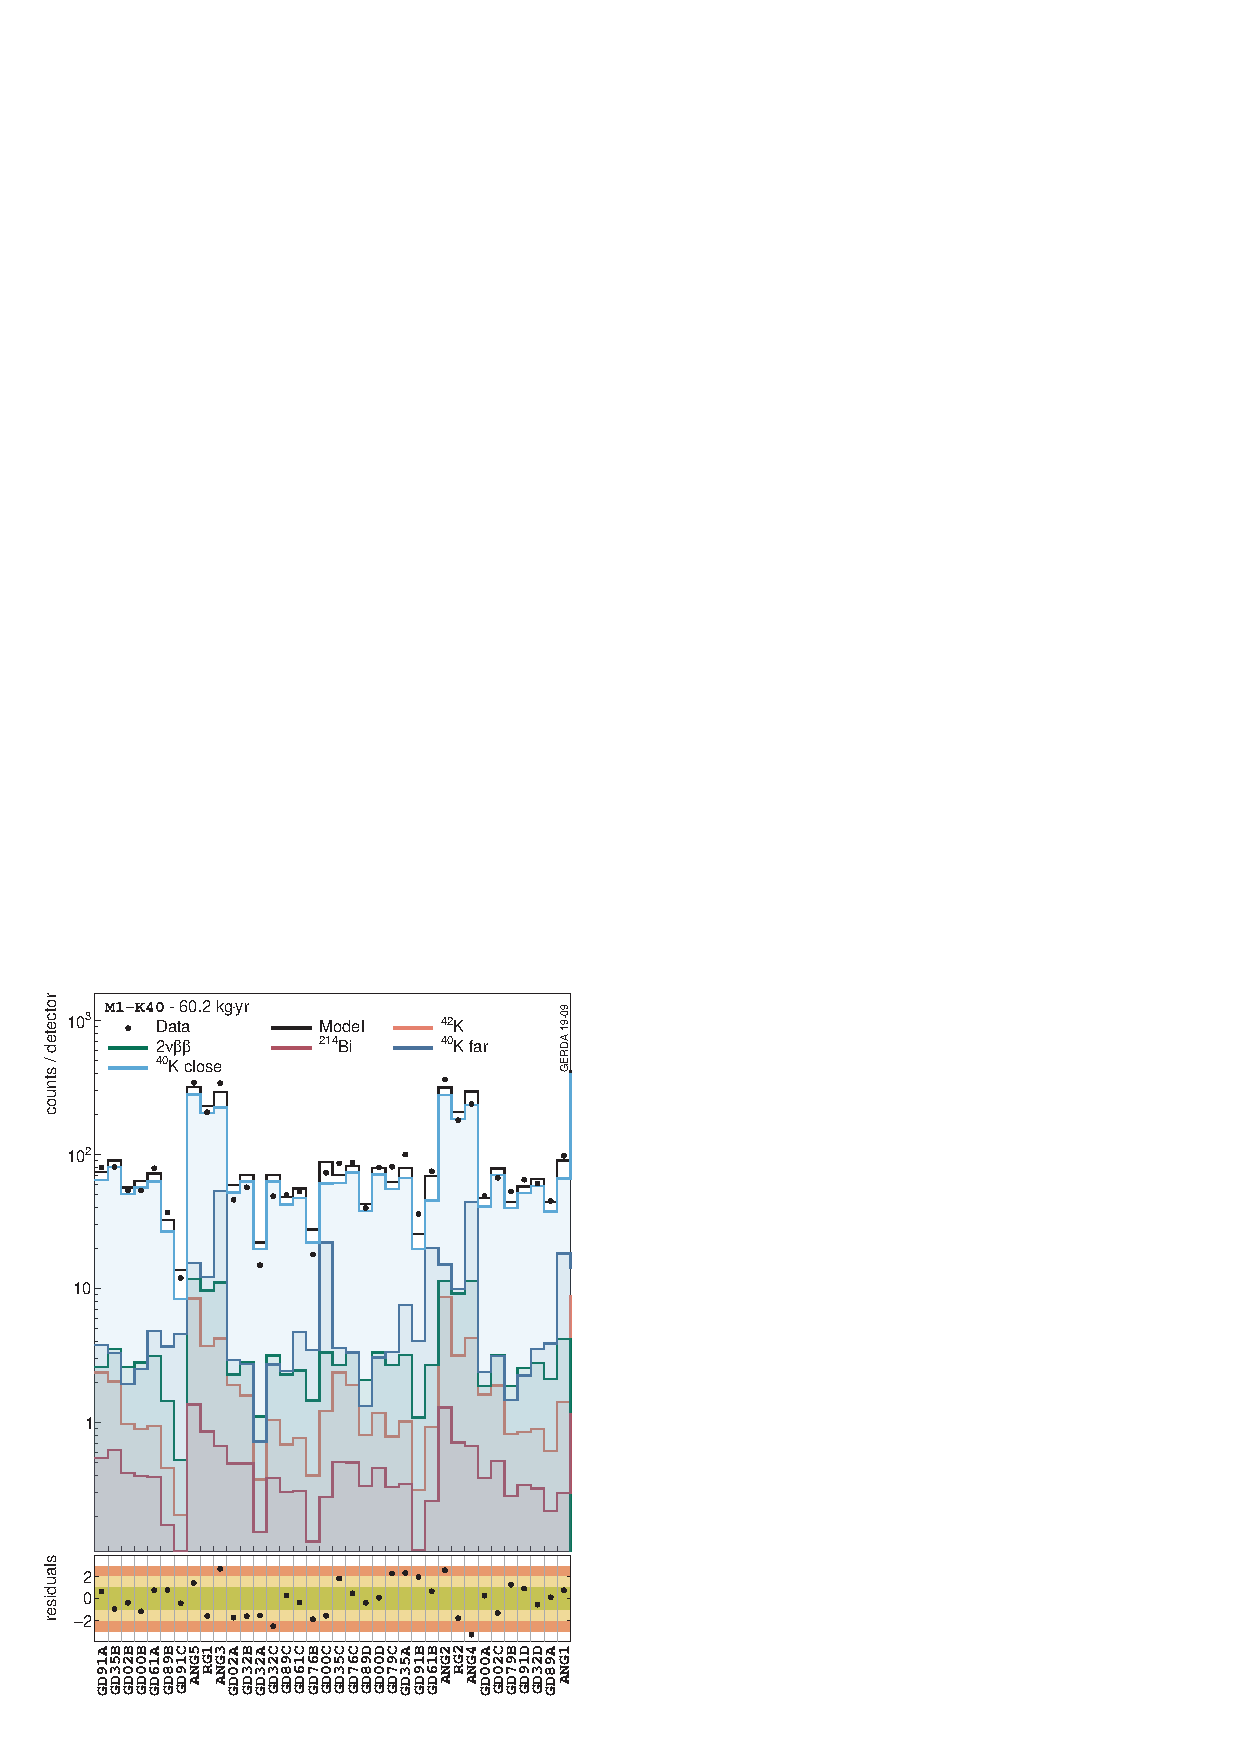
\includegraphics[width=0.45\linewidth]{plots/bkg/raw/ph2/results/kmodel/kmodel-1d-ds0.pdf}
  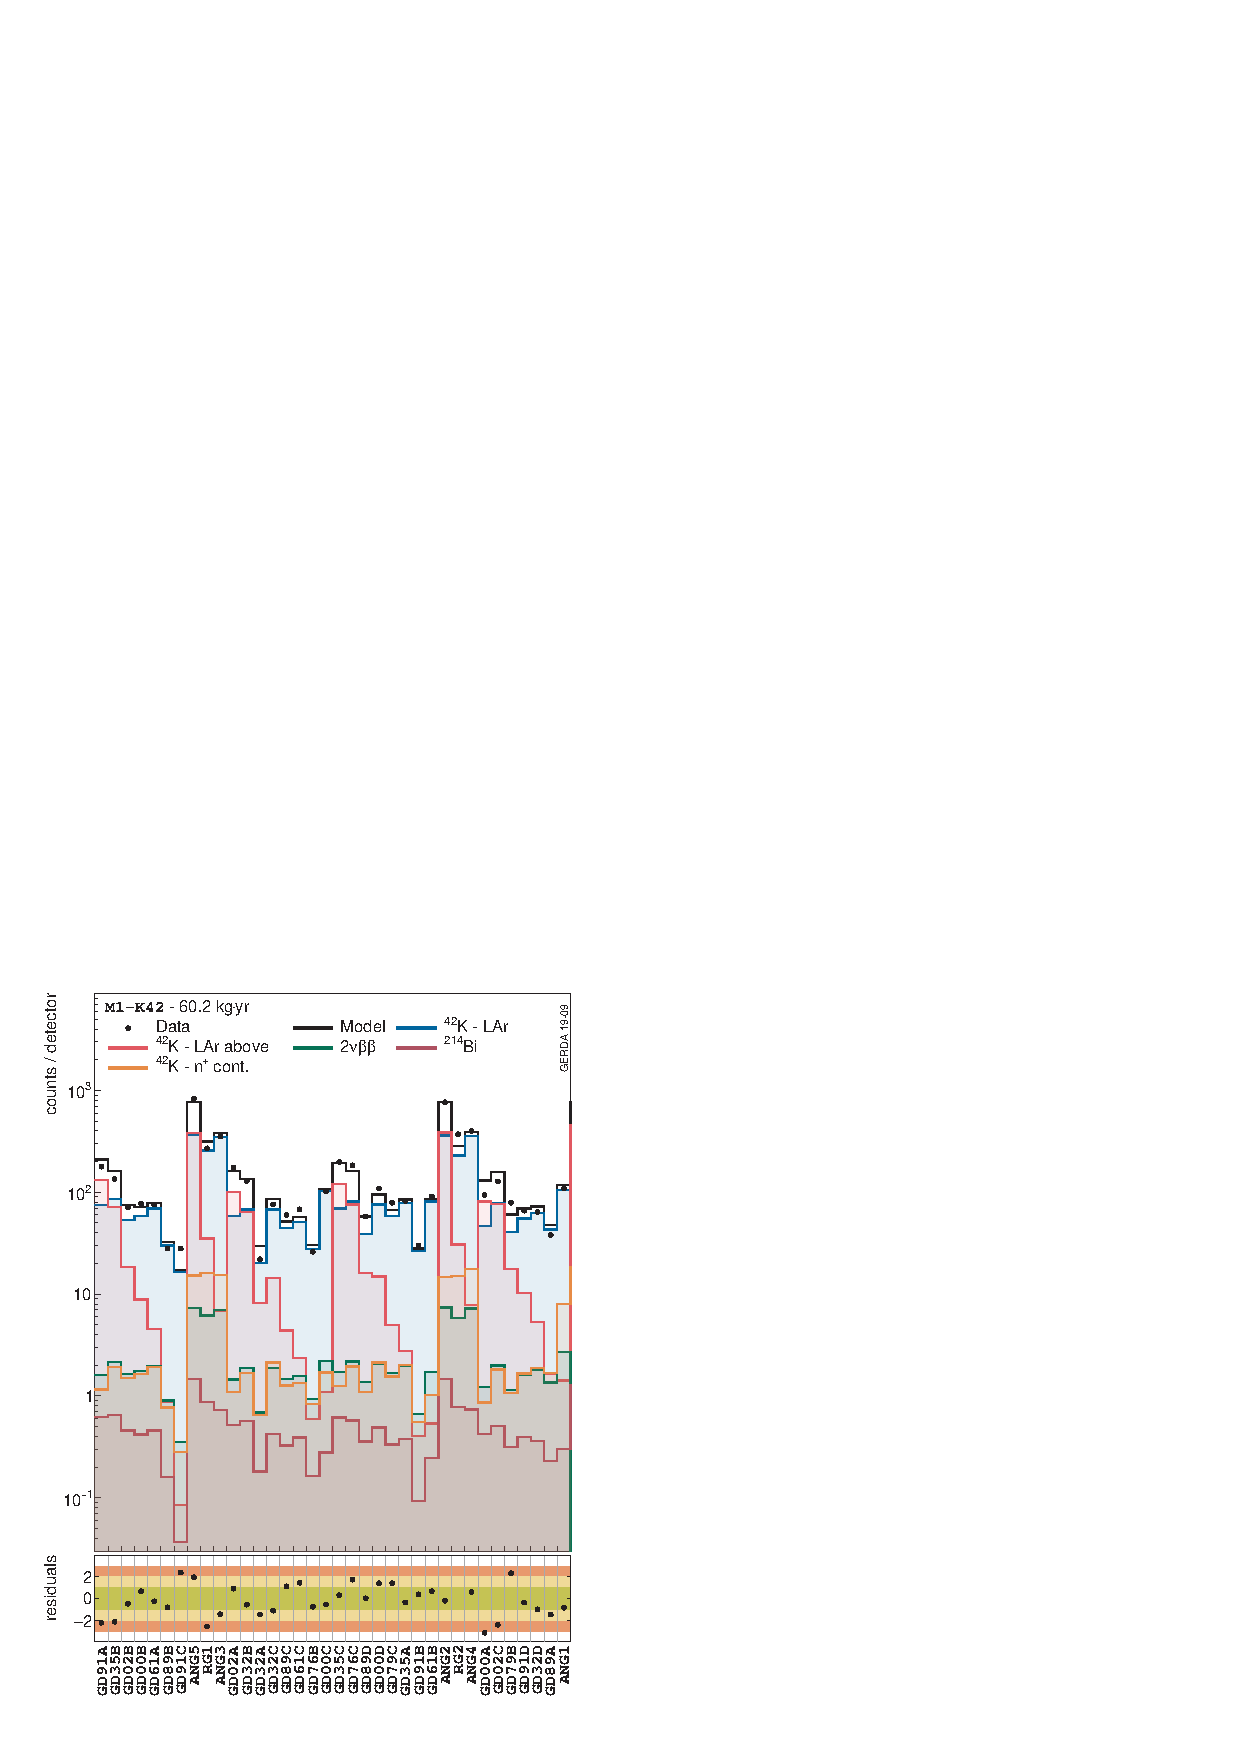
\includegraphics[width=0.45\linewidth]{plots/bkg/raw/ph2/results/kmodel/kmodel-1d-ds1.pdf}
  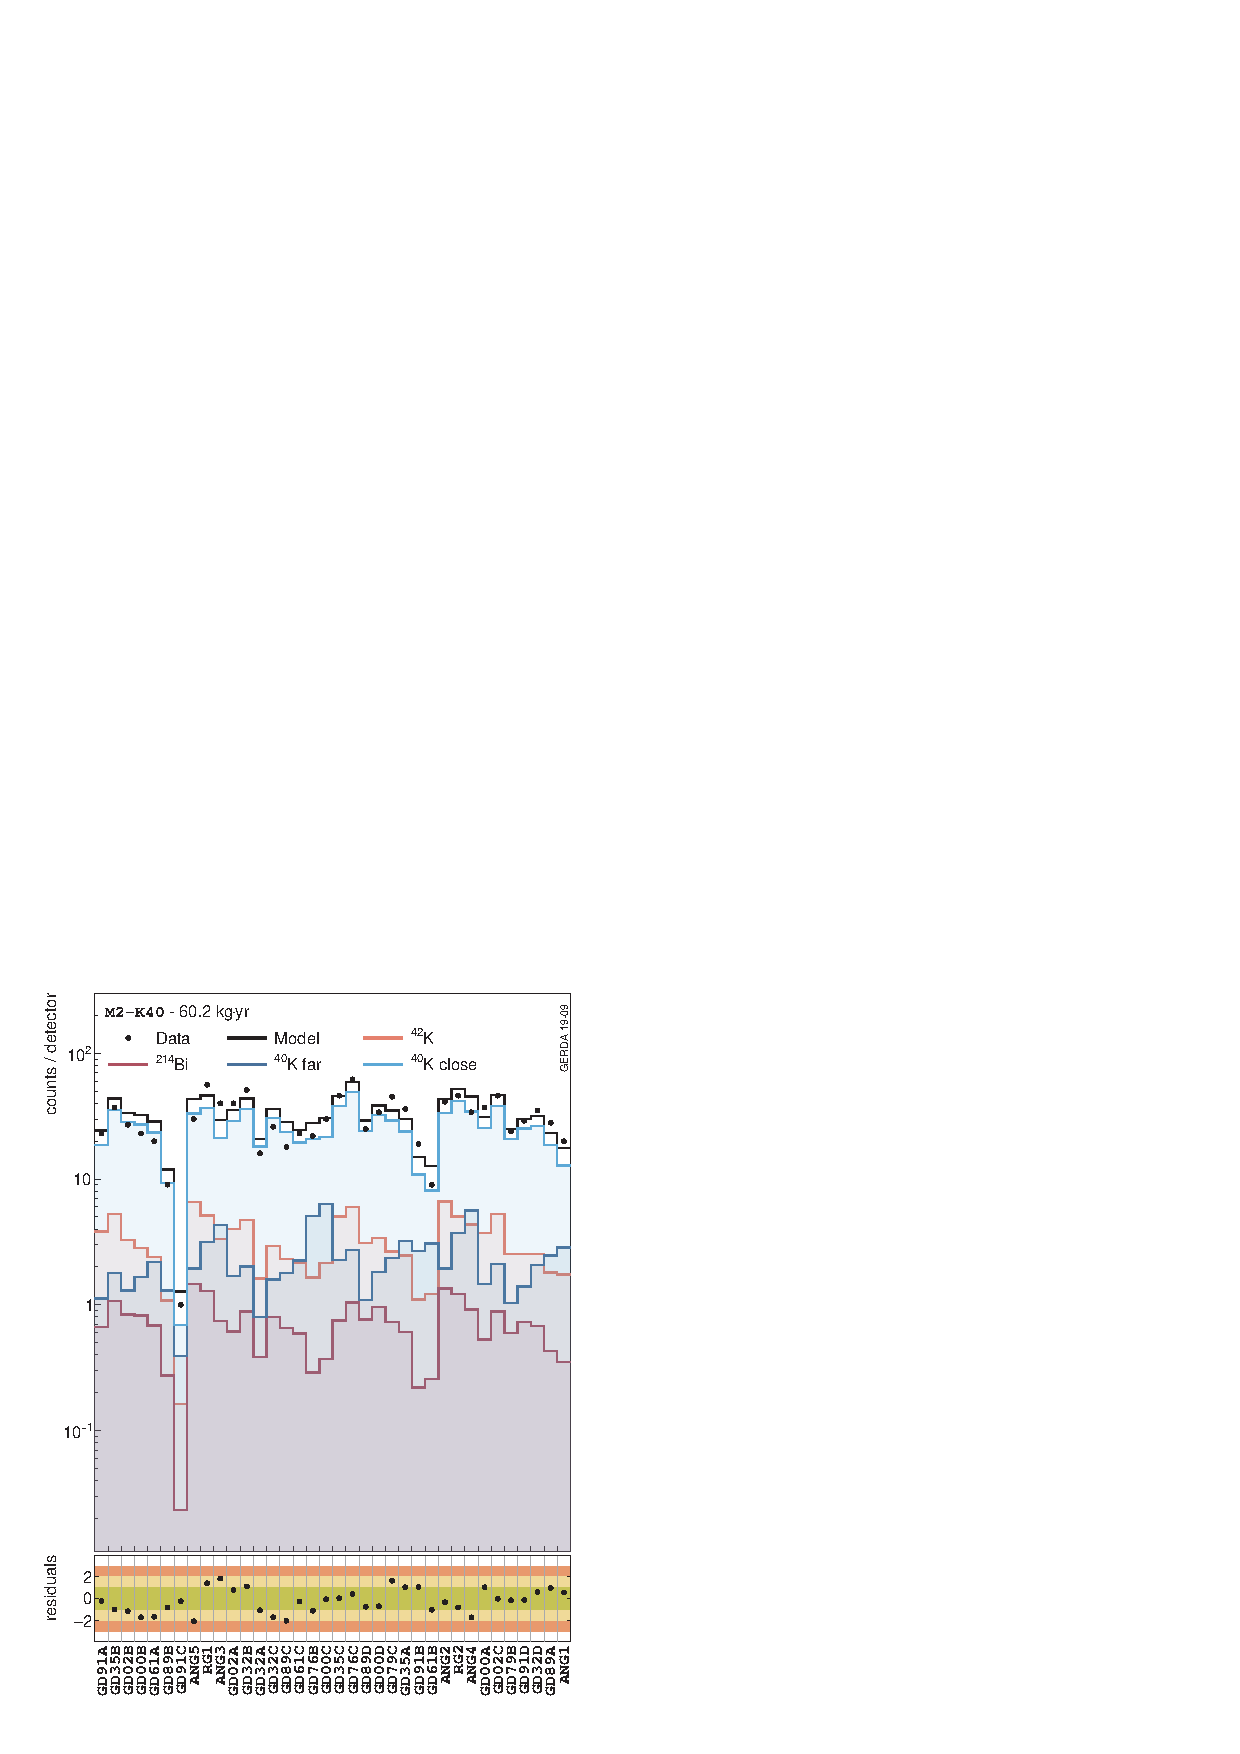
\includegraphics[width=0.45\linewidth]{plots/bkg/raw/ph2/results/kmodel/kmodel-2d-ds5.pdf}
  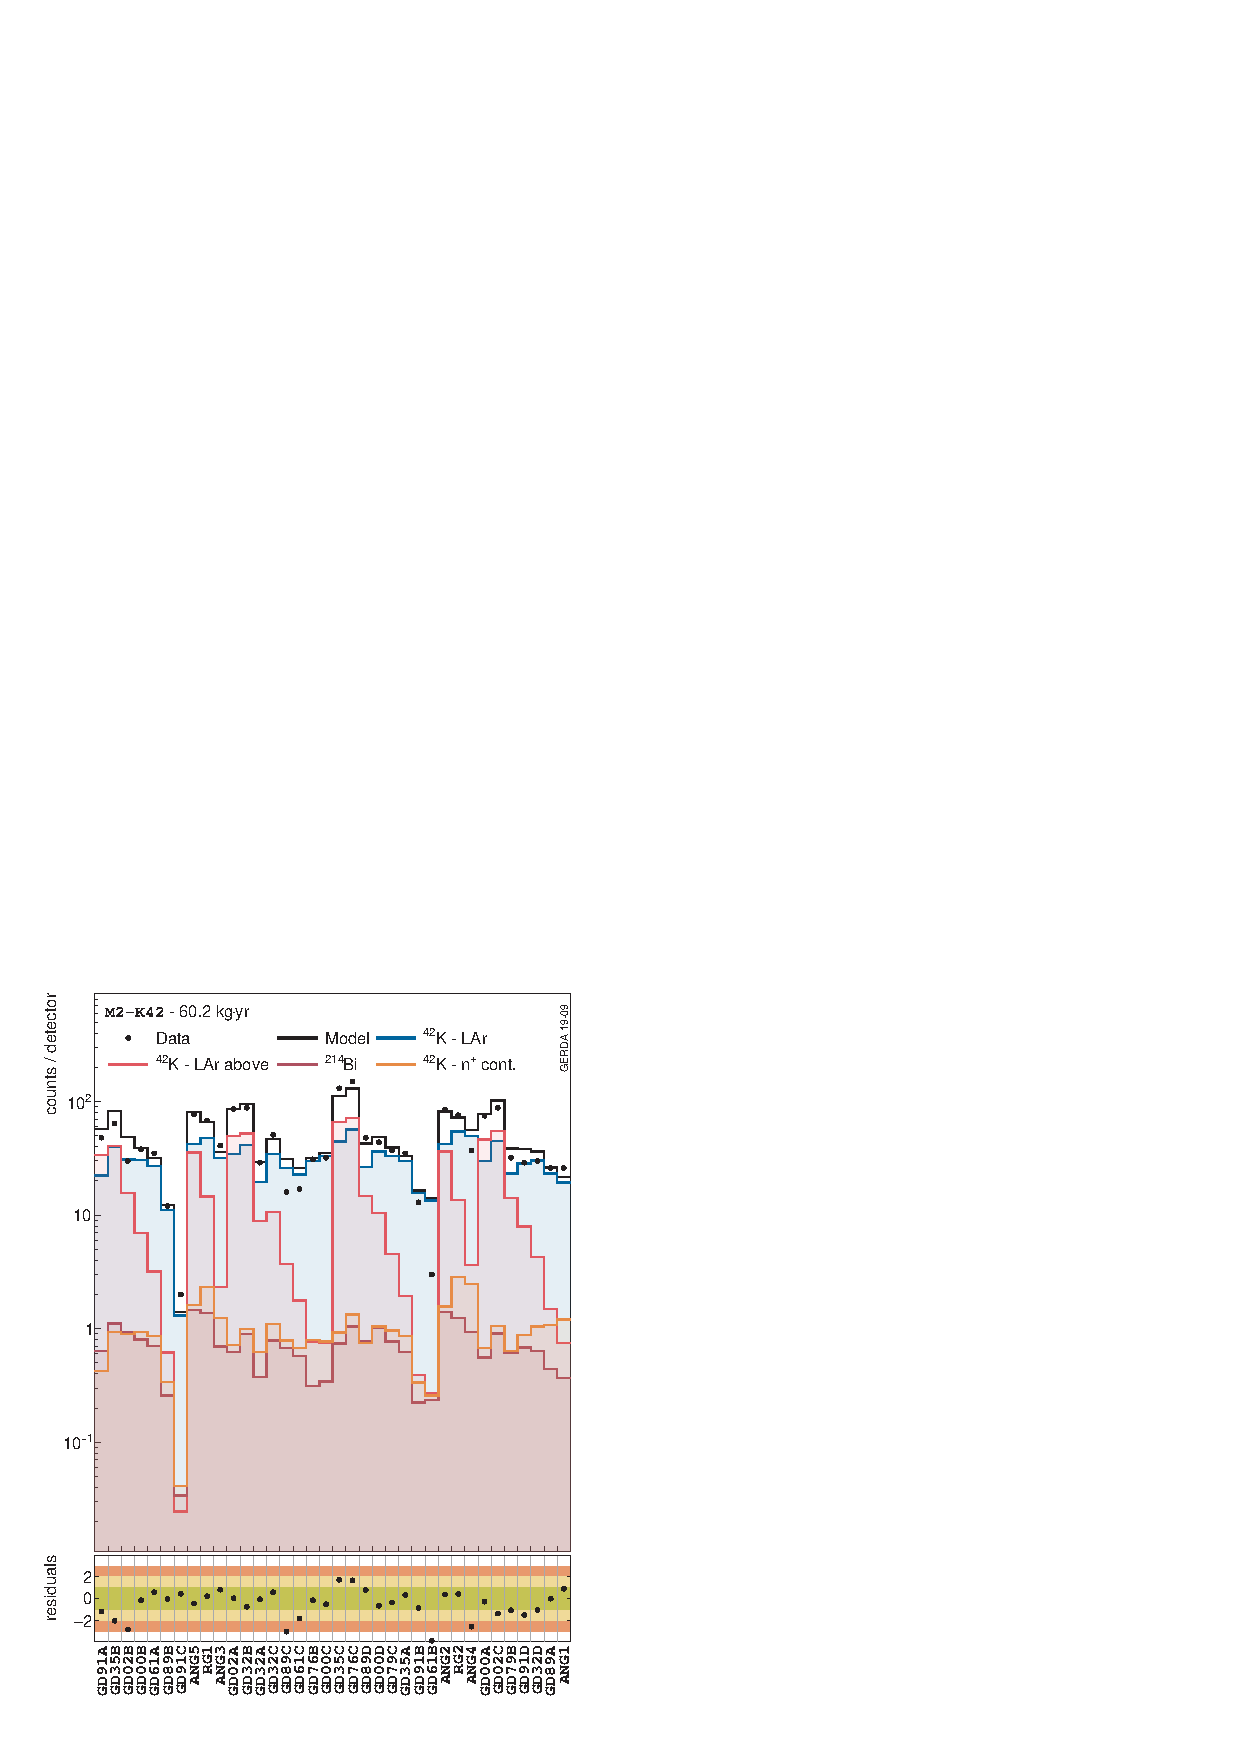
\includegraphics[width=0.45\linewidth]{plots/bkg/raw/ph2/results/kmodel/kmodel-2d-ds6.pdf}
  \caption{%
    Decomposition of the energy windows corresponding to the two potassium lines in
    detector space: single-detector data (top) one-dimensional representation of
    two-detector data (bottom). Some components are merged for visualization purposes: in
    the \m{K40} plots combined components are shown for \kvz\ and \Bih, while \kvn\
    sources are grouped in close (flat cables, holders, mini-shrouds) and far (fibers,
    SiPMs, copper shrouds, front-end electronics) locations from the detector array. To
    visualize the two-detector data the sum of the projections on the two domain axes
    (index $i$ and index $j$) is shown.
  }\label{fig:bkg:raw:ph2:kmodel:base:results}
\end{figure}

\begin{table}
  \centering
  \caption{%
    Summary of the fit parameters estimated with the potassium source tracking analysis
    (base model). The type of prior distribution is indicated with \m{[f]}: flat, \m{[g]}:
    Gaussian. ($\,^{\dagger}$ Tetratex\reg-coated)
  }\label{tab:bkg:raw:ph2:kmodel:base:results}
  \begin{tabular}{rlcccc}
  \toprule
  \mr{2}{source} & \mr{2}{\m{[prior]} location}        & \mr{2}{units} & global & marg. & 68\% C.I. or    \\
                 &                                     &               & mode   & mode  & 90\% upper C.L. \\
  \midrule
  \mr{9}{\kvn}   & \m{[g]} flat cables                 & \mr{9}{mBq}   & 3.29   & 3.25  & $[1.79, 4.72]$  \\
                 & \m{[g]} front-end electronics       &               & 15.7   & 15.9  & $[11.1, 20.1]$  \\
                 & \m{[g]} copper shrouds$^{\dagger}$  &               & 18.4   & 18.1  & $[16.6, 20.0]$  \\
                 & \m{[g]} fiber shroud                &               & 2.82   & 2.81  & $[2.24, 3.38]$  \\
                 & \m{[g]} detector holders            &               & 1.73   & 1.73  & $[1.28, 2.14]$  \\
                 & \m{[g]} mini-shrouds                &               & 1.70   & 1.70  & $[1.60, 1.80]$  \\
                 & \m{[g]} SiPM ring                   &               & 2.50   & 2.73  & $[0.83, 4.13]$  \\
                 & \m{[f]} far from the array          &               & 328    & 322   & $[232,  416]$   \\
                 & \m{[f]} close to the array          &               & 10.8   & 10.8  & $[9.53, 12.1]$  \\
  \midrule
  \mr{4}{\kvz}   & \m{[f]} \nplus\ (BEGe)              & \mr{4}{mBq}   & 0      & 0     & < 0.37          \\
                 & \m{[f]} \nplus\ (Coax)              &               & 0.22   & 0.24  & $[0.12, 0.38]$  \\
                 & \m{[f]} LAr -- above array          &               & 450    & 454   & $[436,  470]$   \\
                 & \m{[f]} LAr -- outside mini-shrouds &               & 2036   & 2009  & $[1915, 2080]$  \\
  \midrule
  \Bih\          & \m{[g]} flat cables                 & mBq           & 1.51   & 1.26  & $[0.93, 1.51]$  \\
%                & \m{[g]} detector holders            &               & 0      & 0     & < 0.35          \\
  \midrule
  \nnbb\         & \m{[f]} germanium                   & $10^{21}$yr   & 1.91   & 1.93  & $[1.86, 2.00]$  \\
  \bottomrule
\end{tabular}

% vim: nowrap

\end{table}

\blocktitle{extended \\ model}
The two components \emph{\kvn\ close to the array} and \emph{\kvz\ in LAr above the array}
are split into 7 sub-components on a string-by-string basis (for the respective pdfs see
\cref{apdx:magepdfs}). Furthermore, we consider a \kvn\ contamination on top of the
central mini-shroud.  The results of this extended analysis are listed in
\cref{tab:bkg:raw:ph2:kmodel:extended:results}. The reader is referred to
\cref{apdx:kmodelplots} for the graphical representation of the background decomposition.
Per-string concentrations of \kvn\ and \kvz\ are visualized also in
\cref{fig:bkg:raw:ph2:kmodel:extended:strings}.  An elevated \kvz\ concentration is found
above the central string while a lower concentration is observed above the adjacent
strings \m{S1} and \m{S6} (string numbers follow the nomenclature used in
\cref{fig:setup:array}). Due to the large number of components the fit yields a high
anti-correlation between the \kvz\ concentration above the outer strings and \m{S7}. This
results in a high uncertainty on the latter fit parameter.
\newpar
The screening measurements do not account for all observed \kvn. In general ICP-MS
screening of the mini-shrouds with respect to \kvn\ is difficult and yielded only a lower
limit. Different measurements seem to indicate different contamination levels of different
mini-shrouds.  Samples of glued nylon yielded the highest potassium contamination. As the
gluing of the nylon mini-shrouds is done manually during installation the amount of glue
and its exact location is hard to control. Hence, an asymmetric distribution is expected.
The \kvn\ content of other close components like holders and cables might also be
asymmetric. The asymmetric \kvn\ contamination is confirmed by the extended potassium
tracking analysis. Also, an additional \kvn\ distribution on the top-lid of the central
mini-shroud is preferred.  The surplus in the far \kvn\ component instead is possibly explained
by setup parts omitted in the model like the PMTs and voltage-dividers of the LAr veto
system. An upper limit of their \kvn\ content, <330~mBq, was estimated from material
screening which is similar to the activity reconstructed for the far \kvn\ component. The
location of the PMTs with respect to the detector array is very similar to the
Tetratex\reg-coated copper-shrouds and their pdfs are, hence, degenerate.

\begin{table}
  \centering
  \caption{%
    Summary of the fit parameters estimated with the potassium source tracking analysis
    (extended model). The type of prior distribution is indicated with \m{[f]}: flat,
    \m{[g]}: Gaussian. ($\,^{\dagger}$ Tetratex\reg-coated)
  }\label{tab:bkg:raw:ph2:kmodel:extended:results}
  \begin{tabular}{rlcccc}
  \toprule
  \mr{2}{source} & \mr{2}{\m{[prior]} location}        & \mr{2}{units} & global & marg. & 68\% C.I. or    \\
                 &                                     &               & mode   & mode  & 90\% upper C.L. \\
  \midrule
  \mr{16}{\kvn}  & \m{[g]} flat cables                 & \mr{16}{mBq}  & 2.33   & 1.08  & $[0.13,2.30]$   \\
                 & \m{[g]} front-end electronics       &               & 14.5   & 14.4  & $[10.2,18.7]$   \\
                 & \m{[g]} copper shrouds$^{\dagger}$  &               & 18.4   & 18.5  & $[16.6,20.0]$   \\
                 & \m{[g]} fiber shroud                &               & 2.83   & 2.77  & $[2.24,3.38]$   \\
                 & \m{[g]} detector holders            &               & 2.57   & 2.29  & $[1.75,2.78]$   \\
                 & \m{[g]} mini-shrouds                &               & 1.70   & 1.70  & $[1.60,1.79]$   \\
                 & \m{[f]} close to \m{S1}             &               & 0.81   & 0.83  & $[0.47,1.28]$   \\
                 & \m{[f]} close to \m{S2}             &               & 2.35   & 2.22  & $[1.83,2.51]$   \\
                 & \m{[f]} close to \m{S3}             &               & 0      & 0     & < 0.50          \\
                 & \m{[f]} close to \m{S4}             &               & 2.58   & 2.55  & $[2.10,3.02]$   \\
                 & \m{[f]} close to \m{S5}             &               & 0.97   & 0.85  & $[0.56,1.16]$   \\
                 & \m{[f]} close to \m{S6}             &               & 1.86   & 1.89  & $[1.46,2.30]$   \\
                 & \m{[f]} close to \m{S7}             &               & 0      & 0     & < 2.92          \\
                 & \m{[f]} \m{S7} mini-shroud (top)    &               & 2.09   & 1.83  & $[1.26,2.40]$   \\
                 & \m{[g]} SiPM ring                   &               & 2.44   & 2.32  & $[0.83,4.02]$   \\
                 & \m{[f]} far from the array          &               & 390    & 374   & $[280,468]$     \\
  \midrule
  \mr{10}{\kvz}  & \m{[f]} \nplus\ (BEGe)              & \mr{10}{mBq}  & 0.15   & 0.19  & $[0.05,0.37]$   \\
                 & \m{[f]} \nplus\ (Coax)              &               & 0.22   & 0.26  & $[0.12,0.41]$   \\
                 & \m{[f]} LAr -- above \m{S1}         &               & 0      & 0     & < 0.80          \\
                 & \m{[f]} LAr -- above \m{S2}         &               & 2.22   & 2.96  & $[2.21,3.63]$   \\
                 & \m{[f]} LAr -- above \m{S3}         &               & 1.20   & 1.57  & $[1.06,2.16]$   \\
                 & \m{[f]} LAr -- above \m{S4}         &               & 1.43   & 1.89  & $[1.33,2.41]$   \\
                 & \m{[f]} LAr -- above \m{S5}         &               & 1.49   & 1.91  & $[1.38,2.73]$   \\
                 & \m{[f]} LAr -- above \m{S6}         &               & 0      & 0     & < 1.21          \\
                 & \m{[f]} LAr -- above \m{S7}         &               & 10.4   & 7.84  & $[4.95,9.83]$   \\
                 & \m{[f]} LAr -- outside mini-shrouds &               & 2083   & 2058  & $[1960,2145]$   \\
  \midrule
  \Bih\          & \m{[g]} flat cables                 & mBq           & 1.60   & 1.41  & $[1.14,1.66]$   \\
%                & \m{[g]} detector holders            &               & 0      & 0     & < 0.26          \\
  \midrule
  \nnbb\         & \m{[f]} germanium                   & $10^{21}$yr   & 1.89   & 1.89  & $[1.83,1.97]$   \\
  \bottomrule
\end{tabular}

\end{table}

\begin{figure}
  \centering
  \includegraphics[width=0.7\textwidth]{plots/bkg/raw/ph2/results/kmodel/kmodel-asym.pdf}
  \caption{%
    Asymmetry of \kvn\ contaminations (left) close to the array strings (for \m{S7} just
    on the top-lid) and \kvz\ (right) above the detector strings. The inner and outer
    radii of each circle are proportional to the edges of the smallest 68\% C.I. of the
    marginalized posterior distributions. The numerical values can be found in
    \cref{tab:bkg:raw:ph2:kmodel:extended:results}.
  }\label{fig:bkg:raw:ph2:kmodel:extended:strings}
\end{figure}

\section{Full-range analysis}%
\label{sec:bkg:raw:ph2:gmodel}

As described in \cref{sec:bkg:raw:ph2:stat} the \a-event background and
potassium \g\ lines are studied individually and the results are incorporated in the
full-range fit as prior distributions.  The latter consists in a simultaneous fit of the
\Mone\ and the \Mtwo\ data sets. For the final combination of parameters, outlined in this
section, components with a posterior distribution peaked at zero were removed from the
fit. The stability of the results with respect to the bin size and prior distributions was
verified. Changing the prior distribution for fit parameters for which no screening
measurement is available from a flat to an exponential one does not significantly impact
the final posterior distributions. The compatibility of the final model, which includes 34
fit parameters, with data is supported by a \pvalue\ of $\sim$~0.3.
\newpar
The estimated activities of individual components and other parameters of interest are
listed in \cref{tab:bkg:raw:ph2:gmodel:results}. In particular, for each component we
report the global and the marginalized mode of the posterior parameter distribution, along
with its smallest 68\% C.I. The global mode corresponds to the global best fit value while
the marginalized mode is the most probable parameter value when integrating over all other
parameters. The original type of prior distribution is marked with \m{[f]} for flat,
\m{[g]} for Gaussian and \m{[e]} for exponential; the latter two are used if screening
measurements are available. Subsequently, for all \kvn\ and \kvz\ components, the prior
distribution is imported from the potassium-tracking analysis and for \Pbh\ and \Bih\ on
the \pplus\ contact from the reconstructed \Ra\ content from the \a\ events background
analysis.
\newpar
The spectral decomposition of all data sets is shown in
\cref{fig:bkg:raw:ph2:gmodel:results}. For each data set the residual distribution as a
multiple of the expected 1$\sigma$ fluctuation in each bin is displayed. We find for the
\enrBEGeII\ data set 66.4\%, 94.5\% and 99.6\% of points in the 1$\sigma$-, 2$\sigma$- and
3$\sigma$-bands, for the \enrCoaxII\ data set 66.0\%, 94.7\% and 99.8\% and for the
\enrGeII\ data set 70.0\%, 96.1\% and 99.7\%, respectively. Thus, in all three cases the
residuals are normally distributed. No outliers with residuals larger than $3\sigma$ are
found in a $\pm50$~keV window around \qbb\ and the bins exceeding $3\sigma$ do not
correspond to any known \g\ line.

\begin{sidewaystable}
  \centering
  \footnotesize
  \caption{%
    Summary of the analysis parameter estimates. Global mode and marginalized mode, along
    with its smallest 68\% C.I., are reported as representatives of the posterior
    parameter distribution. The number of reconstructed counts in the fit range and the BI
    at \qbb\ prior active background suppression are listed for each component and each
    analysis data set. The original type of prior distribution is marked with \m{[f]} for
    flat, \m{[g]} for Gaussian and \m{[e]} for exponential. ($\,^{\dagger}$
    Tetratex\reg-coated) %
  }\label{tab:bkg:raw:ph2:gmodel:results}
  \newcolumntype{H}{>{\setbox0=\hbox\bgroup}c<{\egroup}@{}}
\newcolumntype{x}[1]{>{\centering\arraybackslash}p{#1}}
\newcommand{\mrr}[2]{\multirow{#1}[1]{*}{#2}}
\newcommand{\mrc}[2]{\multirowcell{#1}{#2}}

\begin{tabular}{%
  r
  l
  c
  S[% global mode
    table-format=4.2,
    table-number-alignment=right,
    table-text-alignment=right,
    table-parse-only
  ]
  r@{ }l% marginalized with 68% CI interval
  S[% screening measurements
    table-number-alignment=left,
    table-text-alignment=left,
    table-parse-only
  ]
  S[% BEGe
    table-format=5.0,
    table-number-alignment=center,
    table-text-alignment=center,
    table-auto-round=true
  ]@{ | }
  l
  S[% Coax
    table-format=4.0,
    table-number-alignment=center,
    table-text-alignment=right,
    table-auto-round
    ]@{ | }
  l
  S[% M2-All
    table-format=4.0,
    table-number-alignment=center,
    table-text-alignment=center,
    table-auto-round
  ]
}
  \toprule
  \mrr{3}{source}      & \mrr{3}{\m{[prior]} location}         & \mrr{3}{units}      & {\mrc{3}{global\\mode}} & \mc{2}{\mrc{3}{marg.~mode\\with 68\% CI}} & {\mrr{3}{screening}} & \mc{5}{model content in fit range | BI at \qbb}                                             \\
                       &                                       &                     &                         &       &                                   &                      & \mc{5}{units: cts | $10^{-3}$\ctsper}                                                       \\
  \cmidrule(lr){8-12}
                       &                                       &                     &                         &       &                                   &                      & \mc{2}{\enrBEGeII}                     & \mc{2}{\enrCoaxII}                     & \enrGeII\ \\
  \midrule
  \mr{2}{\nnbb}        & \m{[f]} \bege\ detectors              & \mr{3}{$10^{21}$yr} &                         &       &                                   & {--}                 &         & \mrc{2}{0}                   &         & \mrc{2}{0}                   &           \\
                       & \m{[f]} \scoax\ detectors             &                     &                         &       &                                   & {--}                 &         & \mrc{2}{0}                   &         & \mrc{2}{0}                   &           \\
                       & \m{[f]} \icoax\ detectors             &                     &                         &       &                                   & {--}                 &         & \mrc{2}{0}                   &         & \mrc{2}{0}                   &           \\
  \midrule
  \mr{3}{\Bil\ + \Tl}  & \m{[e]} flat cables                   & \mr{3}{$\upmu$Bq}   &                         &       &                                   & < 410                &         & \mrc{3}{3.52\\$[3.30,3.76]$} &         & \mrc{3}{2.21\\$[2.03,2.34]$} &           \\
                       & \m{[g]} copper shrouds$^{\dagger}$    &                     &                         &       &                                   & 194 \pm 19           &         &                              &         &                              &           \\
                       & \m{[g]} mini-shrouds                  &                     &                         &       &                                   & 18  \pm 5            &         &                              &         &                              &           \\
  \midrule
  \mr{6}{\Pbh\ + \Bih} & \m{[f]} \pplus\ (BEGe)                & \mr{6}{$\upmu$Bq}   &                         &       &                                   & {--}                 &         & \mrc{6}{2.63\\$[2.50,2.78]$} &         & \mrc{6}{3.16\\$[2.83,3.50]$} &           \\
                       & \m{[f]} \pplus\ (Coax)                &                     &                         &       &                                   & {--}                 &         &                              &         &                              &           \\
                       & \m{[g]} flat cables                   &                     &                         &       &                                   & 660 \pm 210          &         &                              &         &                              &           \\
                       & \m{[g]} copper shrouds$^{\dagger}$    &                     &                         &       &                                   & 532 \pm 53           &         &                              &         &                              &           \\
                       & \m{[g]} mini-shrouds                  &                     &                         &       &                                   & 43  \pm 13           &         &                              &         &                              &           \\
                       & \m{[g]} SiPM-ring                     &                     &                         &       &                                   & 351 \pm 97           &         &                              &         &                              &           \\
  \midrule
  \mr{9}{\kvn}         & \m{[g]} flat cables                   & \mr{9}{mBq}         &                         &       &                                   & 6  \pm 2             &         & \mrc{9}{0}                   &         & \mrc{9}{0}                   &           \\
                       & \m{[g]} front-end electronics         &                     &                         &       &                                   & 13 \pm 4             &         &                              &         &                              &           \\
                       & \m{[g]} copper shrouds$^{\dagger}$    &                     &                         &       &                                   & 18 \pm 2             &         &                              &         &                              &           \\
                       & \m{[g]} fiber shroud                  &                     &                         &       &                                   & 2.9 \pm 0.6          &         &                              &         &                              &           \\
                       & \m{[g]} detector holders              &                     &                         &       &                                   & 2.8 \pm 0.6          &         &                              &         &                              &           \\
                       & \m{[g]} mini-shrouds                  &                     &                         &       &                                   & 1.7 \pm 0.6          &         &                              &         &                              &           \\
                       & \m{[g]} SiPM ring                     &                     &                         &       &                                   & 2 \pm 2              &         &                              &         &                              &           \\
                       & \m{[f]} far from the array            &                     &                         &       &                                   & {--}                 &         &                              &         &                              &           \\
                       & \m{[f]} close to the array            &                     &                         &       &                                   & {--}                 &         &                              &         &                              &           \\
  \midrule
  \mr{4}{\kvz}         & \m{[f]} \nplus\ (BEGe)                & \mr{2}{$\upmu$Bq}   &                         &       &                                   & {--}                 &         & \mrc{4}{5.69\\$[4.58,6.29]$} &         & \mrc{4}{1.29\\$[1.15,1.40]$} &           \\
                       & \m{[f]} \nplus\ (Coax)                &                     &                         &       &                                   & {--}                 &         &                              &         &                              &           \\
                       & \m{[f]} LAr {--} above array          & \mr{2}{Bq}          &                         &       &                                   & {--}                 &         &                              &         &                              &           \\
                       & \m{[f]} LAr {--} outside mini-shrouds &                     &                         &       &                                   & {--}                 &         &                              &         &                              &           \\
  \midrule
  \mr{3}{\Ac}          & \m{[g]} copper shrouds$^{\dagger}$    & \mr{4}{$\upmu$Bq}   &                         &       &                                   & 62 \pm 6             &         & \mrc{4}{0.36\\$[0.31,0.40]$} &         & \mrc{4}{0.33\\$[0.28,0.37]$} &           \\
                       & \m{[e]} detector holders              &                     &                         &       &                                   & < 250                &         &                              &         &                              &           \\
                       & \m{[g]} mini-shrouds                  &                     &                         &       &                                   & 18  \pm  5           &         &                              &         &                              &           \\
  \Co\                 & \m{[e]} flat cables                   &                     &                         &       &                                   & < 250                &         &                              &         &                              &           \\
  \midrule
  \mr{4}{\a\ decays}   & \m{[f]} \Po\ + \Ra\ chain (\bege)     & \mr{3}{cts}         &                         &       &                                   & {--}                 &         & \mrc{4}{3.31\\$[3.12,3.78]$} &         & \mrc{4}{4.76\\$[4.40,5.08]$} &           \\
                       & \m{[f]} \Po\ + \Ra\ chain (\scoax)    &                     &                         &       &                                   & {--}                 &         &                              &         &                              &           \\
                       & \m{[f]} \Po\ + \Ra\ chain (\icoax)    &                     &                         &       &                                   & {--}                 &         &                              &         &                              &           \\
  \bottomrule%
\end{tabular}%

% vim: nowrap
%
\end{sidewaystable}

\begin{figure}
  \centering
  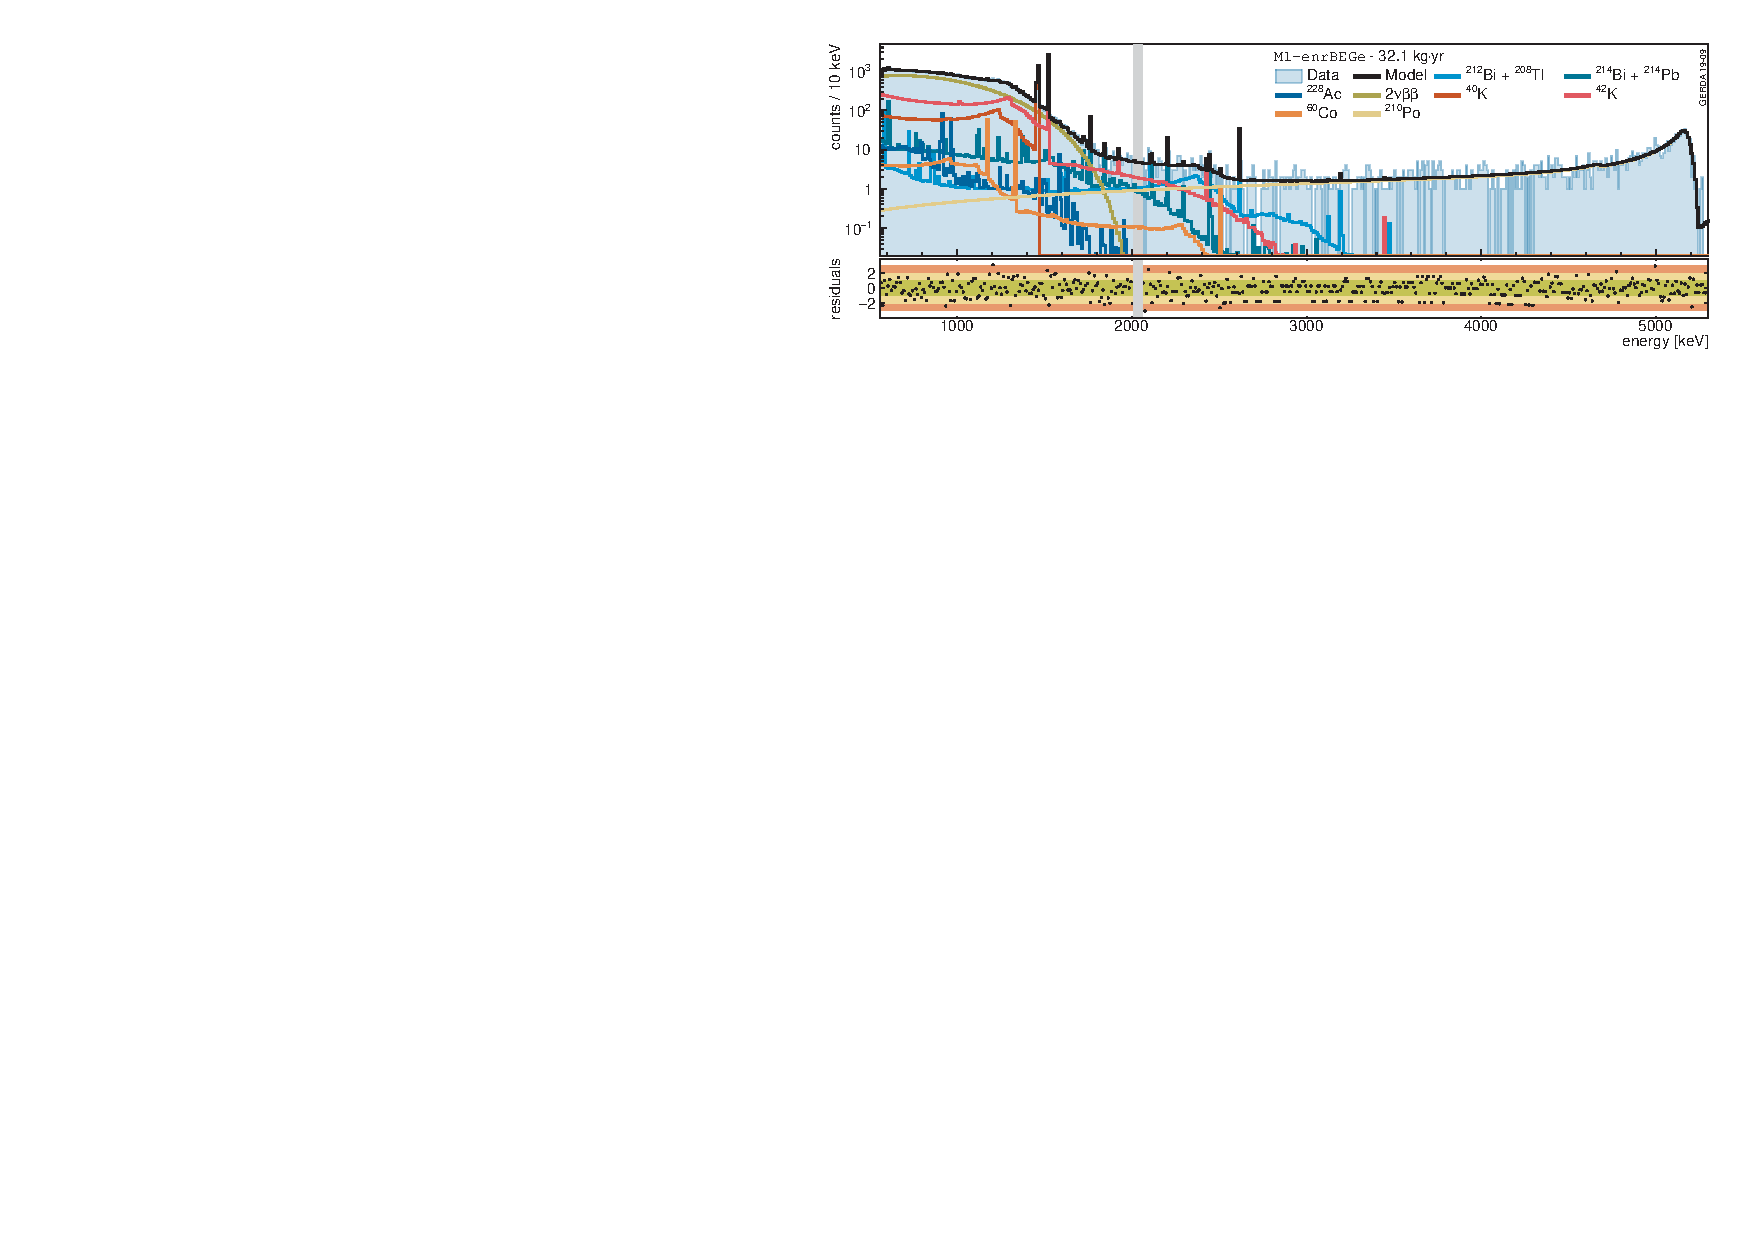
\includegraphics[width=\textwidth]{plots/bkg/raw/ph2/results/gmodel/gmodel-enrBEGe.pdf}
  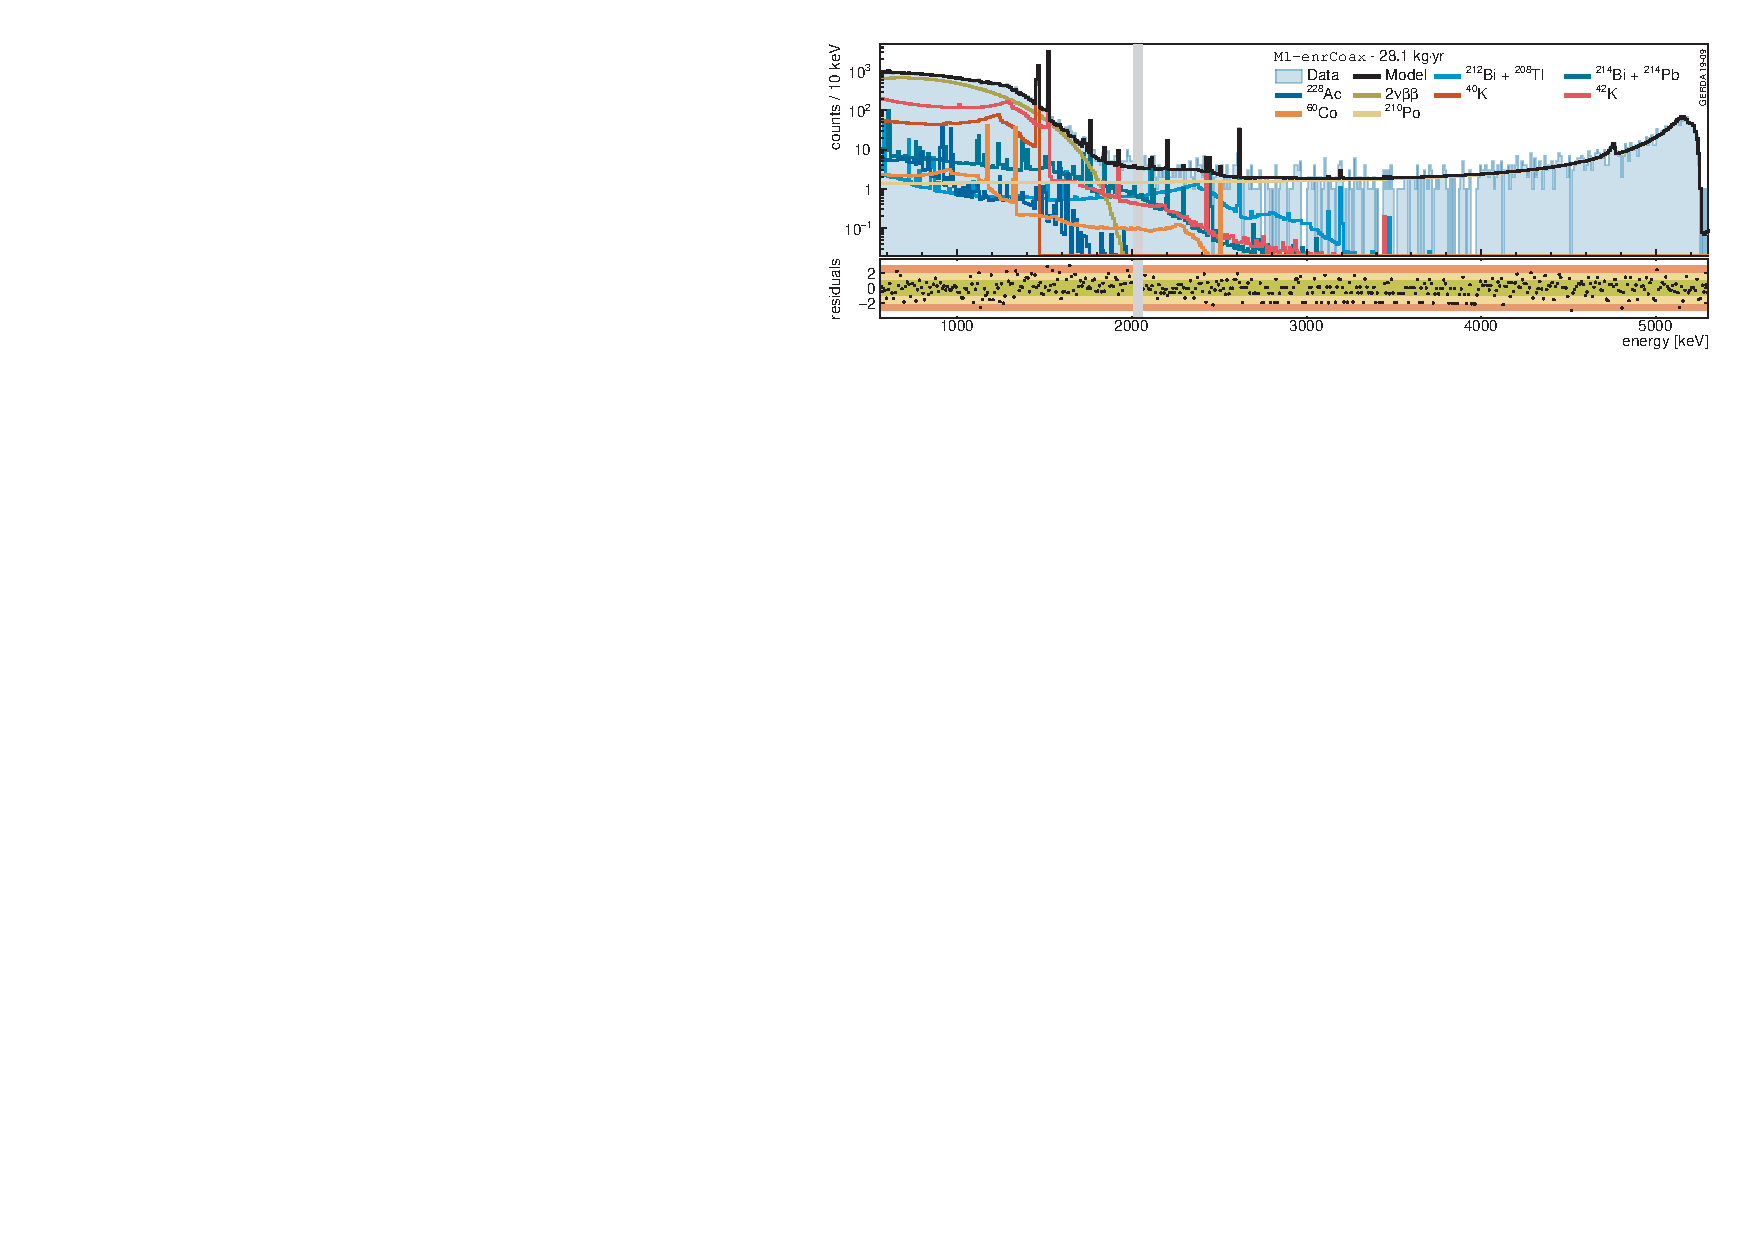
\includegraphics[width=\textwidth]{plots/bkg/raw/ph2/results/gmodel/gmodel-enrCoax.pdf}
  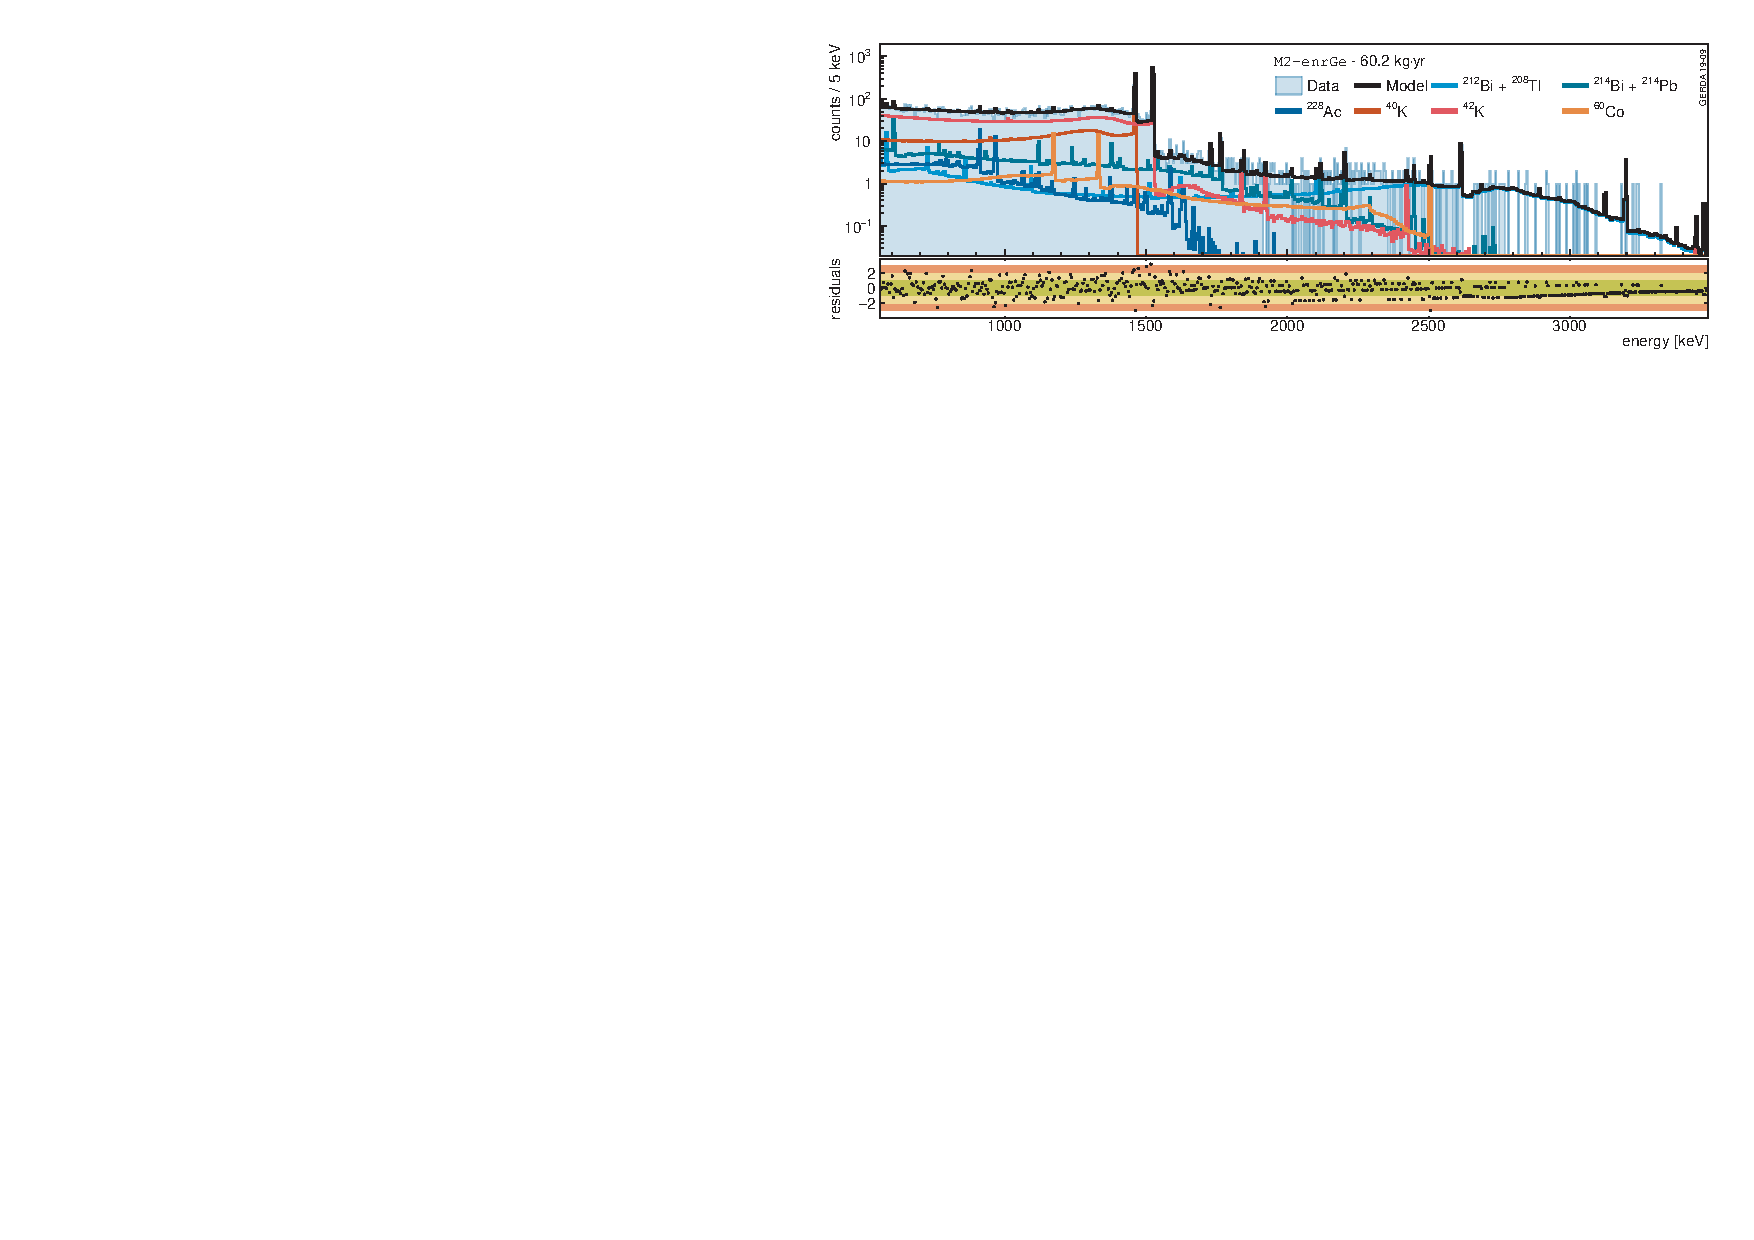
\includegraphics[width=\textwidth]{plots/bkg/raw/ph2/results/gmodel/gmodel-E1plusE2.pdf}
  \caption{%
    Background decomposition of the event energy distributions of the (from top to bottom)
    \enrBEGeII, \enrCoaxII\ and \enrGeII\ data sets.  Components referring to the same
    background source in different locations are summed together for visualization
    convenience. The blinded region $\qbbM \pm 25$~keV is highlighted in gray. In the
    three lower panels displaying the normalized residual distributions the central
    1$\sigma$-, 2$\sigma$- and 3$\sigma$-bands are marked in green, yellow and red,
    respectively. Note that for bins with low expected statistics due to the discrete
    nature of the measured spectrum not all colored bands are
    meaningful~\cite{Aggarwal2011}.%
  }\label{fig:bkg:raw:ph2:gmodel:results}
\end{figure}

\blocktitle{potassium}
The \kvz\ distribution is optimized to best fit the data. In order to disentangle the
\kvz\ \g\  and \b\ components, the volume inside and outside of the mini-shrouds is
separated in the pdf construction. Inside the mini-shrouds a homogeneous distribution is
compatible with the data as well as \kvz\ attached to the detectors contact surfaces. In
the fit model given here, a possible scenario is chosen where all \kvz\ is located on the
\nplus\ surfaces. However, we note that \kvz\ on the \pplus\ appears to partly substitute
the energy-degraded \a\ component in the \enrCoaxII\ data set if introduced in the fit and
predicts a higher total BI around \qbb. The extracted \kvz\ activity on the
\scoax\ \pplus\ contact in this case is $22\pm4$~\mubq\ corresponding to a
contribution to the BI around \qbb\ of $(7\pm1)\cdot10^{-3}~$\ctsper. For the \enrBEGeII\
data set the posterior distribution of a possible \kvz\ component on the \pplus\ contact
is compatible with zero. Outside the mini-shrouds an inhomogeneous distribution of the
\kvz\ decays better explains the observations. Detectors which are located at higher
positions in the strings show an excess of events in the \kvz\ 1525~keV \g\ line which is
compatible with a surplus of \kvz\ located right above the detector array (see
\cref{sec:bkg:raw:ph2:kmodel}). The full-range fit model contains a homogeneous \kvz\
distribution in \textit{LAr, outside the mini-shrouds} which is reconstructed with a specific
activity of $186\pm39$~\mubq/kg plus an additional distribution in the vicinity of the
cables (in \textit{LAr, above the array}).
\newpar
A large fraction of the contamination with \kvn\ in the setup cannot be accounted for by
the screened hardware listed in \cref{tab:bkg:raw:ph2:gmodel:results}. We thus add a close
($\sim$1~cm) and a far ($\sim$50~cm) \kvn\ component with respect to the detector array
which are in fact replica of the pdfs for the mini-shrouds and the Tetratex\reg-coated copper
shrouds. These additional components absorb the excess indicated by the fit, the largest
part of the reconstructed events in the spectra is attributed to impurities close to the
array.
\newpar
The \kvn\ and \kvz\ distributions can be further split into smaller volumes and studied as
an extension of the potassium-tracking analysis (as described in
\cref{sec:bkg:raw:ph2:kmodel}) projected in detector space. The additional \kvn\ component
close to the array and the \kvz\ component above the array are split into 7 sub-components
on a string-by-string basis. The potassium concentration is in general found to be
asymmetric among the detector strings. In particular, a more prominent \kvz\ concentration
is found above the central string. This is consistent with the electrostatic drift of
\kvz\ ions induced by the electric field in the LAr which is generated by the unshielded
high-voltage flat cables biased with about 4~kV. The \kvn\ and \kvz\ spatial analysis
fitting the potassium \g\ lines projected in detector space is presented in full detail in
\cref{sec:bkg:raw:ph2:kmodel}.

\blocktitle{\a\ events}
The \a\ distribution is adjusted to best fit the data. The \Po\ peak at 5.2~MeV is found
to be best described by a mixture of pdfs obtained assuming different \pplus\ contact
thicknesses confirming results of the \phaseone\ background analysis~\cite{Agostini2013a}.
The empirical linear model which is used to describe \a\ events with degraded energy (see
\cref{sec:bkg:raw:ph2:amodel}), extends down to \qbb\ and below. For the \enrBEGeII\ data
set \a\ events are efficiently isolated using pulse shape discrimination (PSD) techniques.
The compatibility of the degraded-energy \a\ component with \a\ events identified by PSD
was checked and is found consistent.  All details about the \a\ events analysis can be
found in \cref{sec:bkg:raw:ph2:amodel}.

\blocktitle{\nnbb}
Most counts in the fit range are attributed to the \nnbb\ decay of \gesix; in fact its
continuous distribution dominates the spectrum up to almost 1.9~MeV. Here, we base the
\nnbb\ half-life estimate on the \enrBEGeII\ data set only. An additional parameter,
$\delta^{2\nu}$, parametrizes the observed discrepancy to the value solely derived from
the \enrCoaxII\ data set. The value of $\delta^{2\nu}$ extracted from the fit amounts to a
surplus of 5\% of \nnbb\ counts observed in \enrCoaxII.  It mainly quantifies the
systematic biases between the active volume determination methods of the two detector
types. The \bege\ detectors active volume measurements are affected by a smaller
systematic uncertainty than the \scoax\ detectors~\cite{Agostini2013a, Agostini2019}.
Hence, the extracted \nnbb\ half-life, based on the \enrBEGeII\ data set and given here
only with statistical uncertainties, amounts to $\thalftwoM = (2.03 \pm 0.02) \cdot
10^{21}$~yr. A detailed discussion follows in \cref{sec:bkg:raw:ph2:discussion}.

\blocktitle{other}
Smaller contributions to the background model in the full energy range are attributed to
\Pbh\ and \Bih\ from the \Uh\ decay chain, \Ac, \Bil\ and \Tl\ from the \Thh\ decay chains
and \Co. With a total contribution in the fit range of $10^{-3}$~cts/keV for both the
\enrBEGeII\ and \enrCoaxII\ data set \Pa\ gives negligible contribution to the spectra and
is therefore dropped from the full-range fit model. The central values preferred in the
full-range fit are driven by screening measurements and the spectral contributions are all
fully accounted for by the listed hardware components. The only exception is \Pbh\ and
\Bih\ where a minor contribution is added on the p$^+$ contact expected from the
observation of \a\ events belonging to the \Ra\ decay chain.

\blocktitle{background \\ at \qbb}
The background model describes the individual contributions to the total BI around \qbb\
prior active background suppression (see \cref{fig:bkg:raw:ph2:gmodel:results:roi}).
The BI is defined as the number of counts over exposure and energy in the energy window
from 1930~keV to 2190~keV excluding the region around \qbb\ ($\qbbM \pm 5$~keV) and the
intervals $2104 \pm 5$~keV and $2119 \pm 5$~keV, which correspond to known \g\ lines from
\Tl\ and \Bih. The values for each background contribution are given in
\cref{tab:bkg:raw:ph2:gmodel:results}. The dominating background contribution around \qbb\
in the \enrBEGeII\ data set come from \kvz. Isotopes from the \Thh\ decay chain, \a\
particles mainly with degraded energy and isotopes from the \Uh\ decay chain contribute
about equally. The estimated total BIs extracted from the marginalized posterior
distributions are $\stat{16.04^{+0.78}_{-0.85}} \cdot 10^{-3}$~\ctsper\ for the
\enrBEGeII\ data set and $\stat{14.68^{+0.47}_{-0.52}} \cdot 10^{-3}$~\ctsper\ for the
\enrCoaxII\ data set.

\begin{figure}
  \centering
  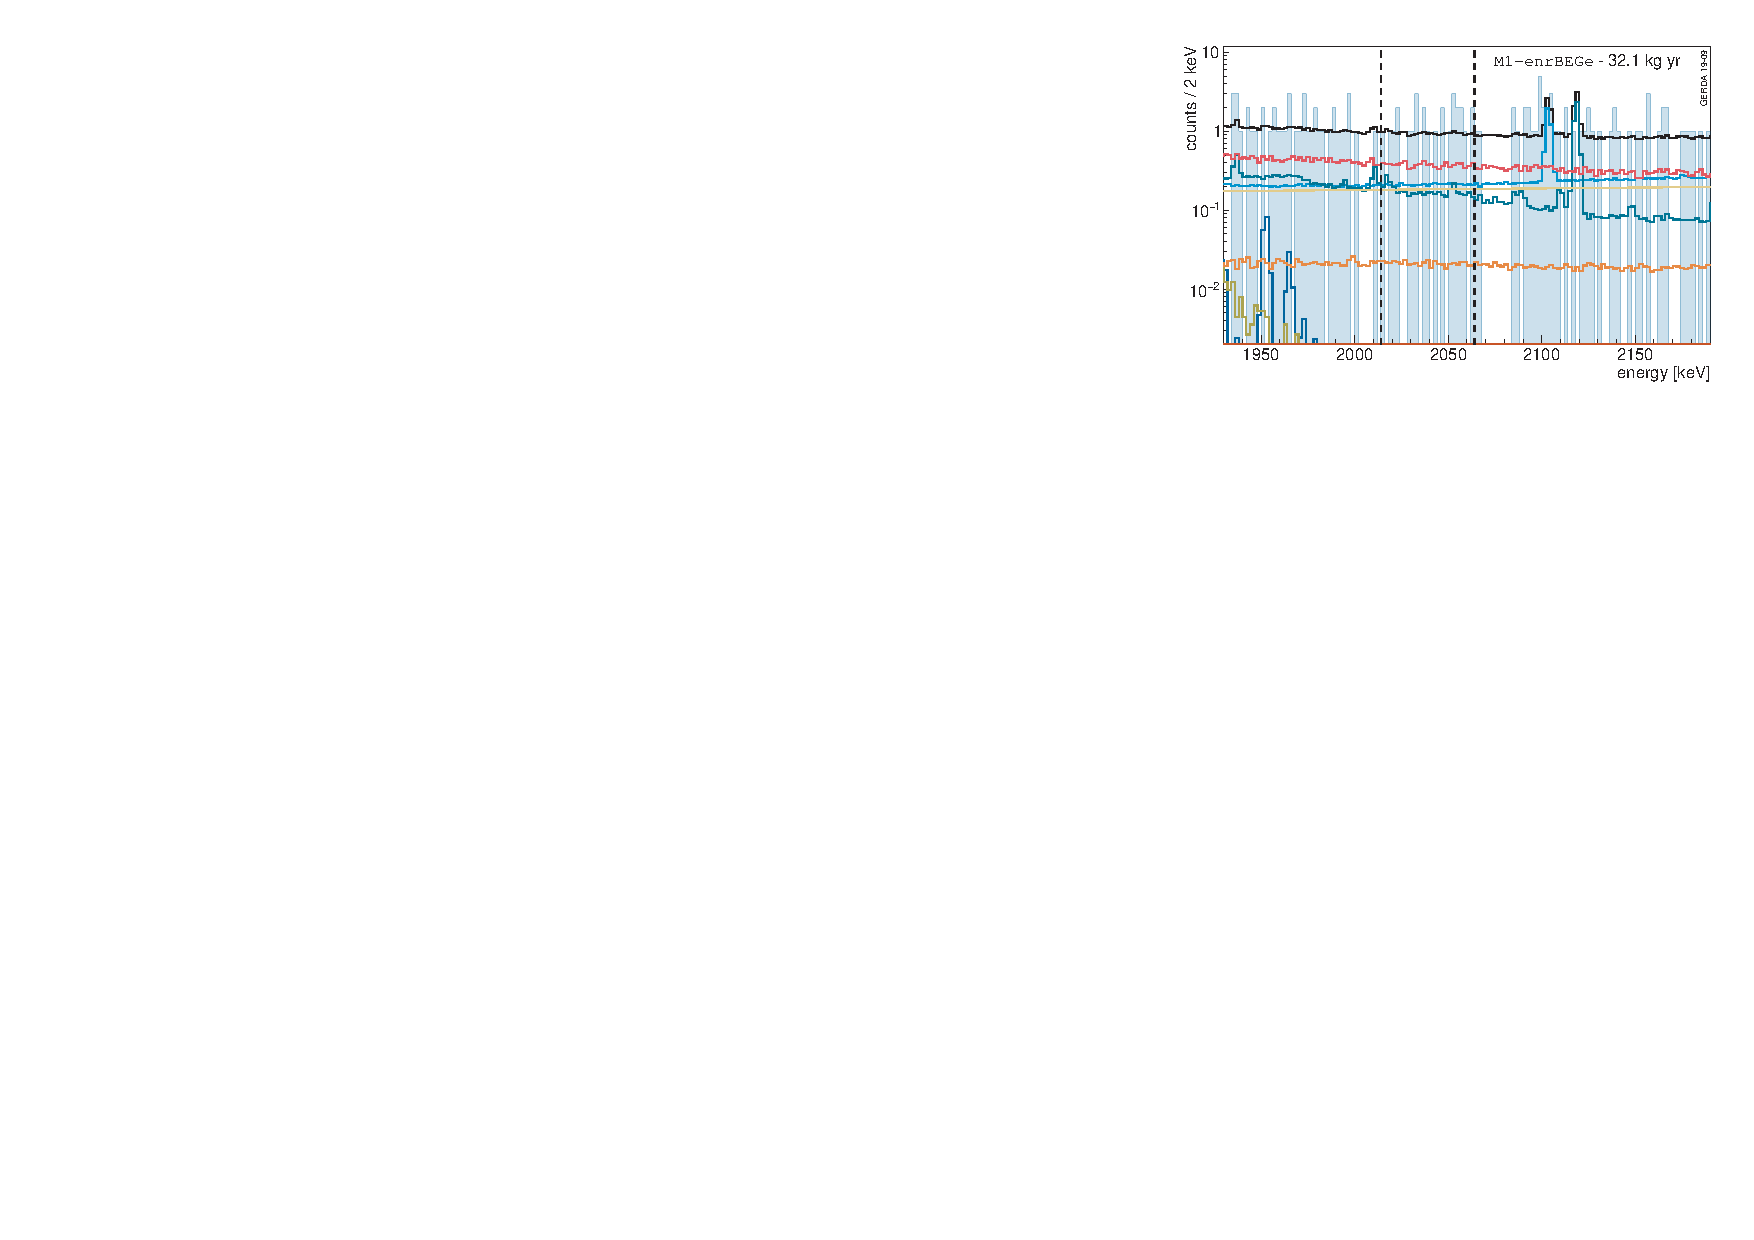
\includegraphics[width=0.45\linewidth]{plots/bkg/raw/ph2/results/gmodel/gmodel-roi-enrBEGe.pdf}
  \hspace{12pt}
  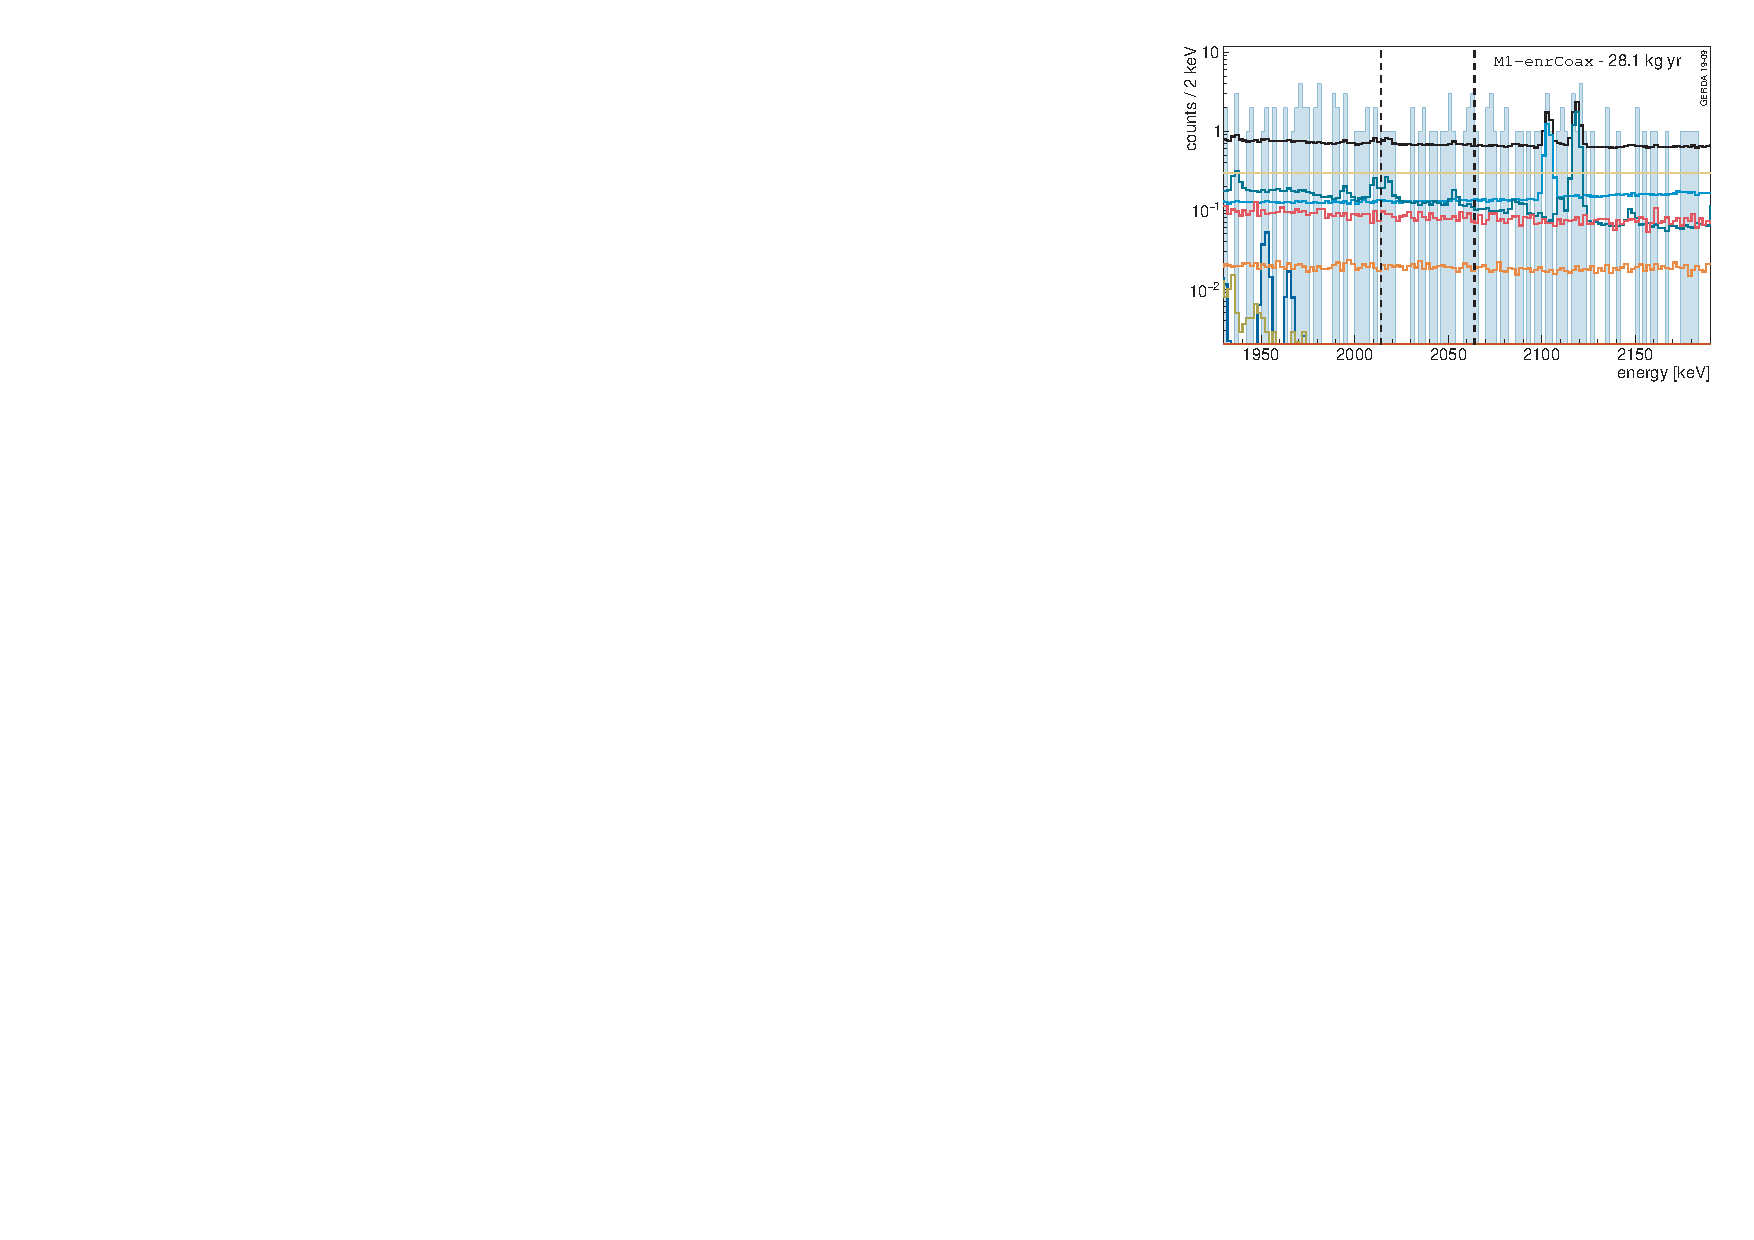
\includegraphics[width=0.45\linewidth]{plots/bkg/raw/ph2/results/gmodel/gmodel-roi-enrCoax.pdf}
  \caption{%
    Background decomposition for the \enrBEGeII\ (left) and the \enrCoaxII\ (right) data
    sets in the background window between 1930~keV and 2190~keV after data unblinding. The
    previously blinded window ($\qbbM \pm 25$~keV) is indicated by two dashed lines.  The
    background distribution before active background suppression in the \onbb\ analysis
    window can be well approximated with a constant function. For color code see
    \cref{fig:bkg:raw:ph2:gmodel:results}.%
  }\label{fig:bkg:raw:ph2:gmodel:results:roi}

  \includegraphics{plots/bkg/raw/ph2/results/gmodel/BI-bars.pdf}
  \caption{%
    Background decomposition in the BI analysis window around \qbb.
  }\label{fig:bkg:raw:ph2:gmodel:results:roibars}
\end{figure}

\section{Discussion}%
\label{sec:bkg:raw:ph2:discussion}

In general, the marginalized posterior distributions and the results of the material assay
measurements are in very good agreement. The only exception is constituted by the \kvn\
activity, which cannot be explained by the available prior information and is fit with the
additionally introduced components far and close to the detector array. The \kvz\ and \a\
event distributions, as already mentioned, cannot be constrained by screening measurements
and are adjusted to best fit the data.  The background model is not completely free of
parameter correlations. As shown in \cref{fig:bkg:raw:ph2:pdfs:gmodel} several pdfs of the
same source of background located in different structural components are very similar and
thus generate correlations. Most of them have been resolved by introducing prior
distributions based on the screening measurements.  However, a few anti-correlations
persist which are listed in \cref{tab:bkg:raw:ph2:corr}.

\begin{table}
  \centering
  \caption{%
    Correlations between fit components relative to the same background contamination in
    different locations.
  }\label{tab:bkg:raw:ph2:corr}
  \begin{tabular}{cccc}
    \toprule
    contamination & location 1                  & location 2         & correlation \\
    \midrule
    \Bih\ + \Pbh\ & mini-shrouds                & flat cables        & -0.43 \\
    % \midrule
    \mr{2}{\kvn}  & flat cables                 & detector holders   & -0.45 \\
                  & flat cables                 & close to the array & -0.63 \\
    % \midrule
    \mr{2}{\kvz}  & LAr -- outside mini-shrouds & \nplus\ contact    & -0.42 \\
                  & LAr -- outside mini-shrouds & LAr -- above array & -0.56 \\
    \bottomrule
  \end{tabular}
\end{table}

\blocktitle{\kvz}
For what concerns \kvz\ in the LAr volume outside the mini-shrouds, the adoption of an
additional pdf for \kvz\ above the detector array is purely motivated by the empirical
observation of an excess of background events in the top detectors. The prior knowledge is
indeed limited by the fact that the \kvz\ ions undergo drift due to the electrical fields
surrounding the detectors and high-voltage cables. Also, due to thermal gradients they can
be displaced by convection. With that considered, the presence of unshielded high-voltage
cables above the detector array can perhaps explain the excess of \kvz\ observed in this
region. A more detailed investigation of the \kvz\ distribution in LAr is not pursued any
further, as the full-range fit is inevitably not sensitive to such effects. A more
sophisticated Monte Carlo model would in fact not significantly impact the \kvz\ pdfs
shape. Nevertheless, some considerations are presented in the contest of the potassium
tracking analysis, which is the only analysis presented here that could shed some light on
the problem (see \cref{sec:bkg:raw:ph2:kmodel}). An explanation for \kvz\ on the \pplus\
contact being rejected for the \enrBEGeII\ data set but potentially present in the
\enrCoaxII\ data can be the specific bore-hole geometry of the semi-coaxial detectors.
\kvz\ produced inside the hole cannot easily escape and is trapped close to the \pplus\
contact.

\blocktitle{background \\ window}
For each source of background the contribution to the BI at \qbb\ prior to active
background reduction is listed in \cref{tab:bkg:raw:ph2:gmodel:results}. The statistical
uncertainties on the single contributions to the BI are generally of the order of 10\% or
lower, with the exception of \kvz\ and energy-degraded \a\ events, for which the
uncertainty is roughly doubled. The two contributions are affected by a higher uncertainty
because they are not bound by screening measurements.
\newpar
The background event distribution in the \onbb\ analysis window can be well approximated
with a constant function (see \cref{fig:bkg:raw:ph2:gmodel:results:roi}).  With this
assumption, the BIs extracted from data are $16.4^{+1.7}_{-1.6} \cdot 10^{-3}$~\ctsper\
for \enrBEGeII\ and $15.4^{+1.8}_{-1.6} \cdot 10^{-3}$~\ctsper\ for the \enrCoaxII\ data
set.  These values agree well with the background model description presented in
\cref{sec:bkg:raw:ph2:gmodel}. The BIs prior to further analysis cuts and before the
upgrade of the \gerda\ experiment to \phasetwo\ can be found in
reference~\cite{Agostini2013c}. For the \enrCoaxII\ data set the BI prior to the upgrade
of $(18 \pm 2) \cdot 10^{-3}$~\ctsper\ is very consistent with the values presented here.
The BI of the \enrBEGeII\ data set instead is substantially improved from a \phaseone\
value of $42^{+10}_{-8} \cdot 10^{-3}$~\ctsper\ to a value which is at least $2.5\times$
smaller in \phasetwo\ despite a significant increase of inactive hardware
mass.\footnote{Note the slight difference of the \enrBEGeII\ analysis data set presented
here and the data set used for \onbb\ analysis for which the improvement in the BI is
slightly higher ($3\times$ better BI). This is due to discarded \bege\ data for which no
PSD can be applied.} Contributions to the BI from all isotopes have been improved with
respect to \phaseone\ with the exception of background introduced by \a\ surface events.
The most drastic improvement is notable for \kvz\ for which the BI contribution for the
\bege\ detectors appears four times smaller than before the upgrade to \phasetwo.

\blocktitle{\nnbb\ \\ systematics}
As mentioned in \cref{sec:bkg:raw:ph2:gmodel}, the extracted \nnbb\ half-life estimate is
based on the \enrBEGeII\ data set only. The additional parameter $\delta^{2\nu}$ mainly
quantifies the systematic biases between the active volume determination methods of the
two detector types. The full charge collection depth (FCCD), which determines the active
volume of a detector, was studied extensively in a detector characterization campaign for
the \bege\ detectors~\cite{Agostini2015e, Agostini2019}. The estimate of the FCCD used in
this analysis is based on measurements using an \Am\ source with characteristic \g\ lines
at 60~keV, 99~keV and 103~keV.  However, the FCCD was also measured using a \Co\ source
with characteristic \g\ energies of 1173~keV and 1332~keV. The latter FCCD$_\text{Co}$ is
systematically higher (about 3\%) with respect to the FCCD$_\text{Am}$. The discrepancy
could be explained by an energy dependence of the initial charge-carrier cloud size inside
the detector but the actual impact on the active volume is still under investigation.  For
the \scoax\ detectors only FCCD values determined with a \Co\ source are available.
Considering the systematic uncertainties affecting the determined active \gesix\ exposures
of the \enrBEGeII\ and \enrCoaxII\ data sets (1.8\% and 5\% respectively, see
\cref{tab:bkg:raw:ph2:datasets}) $\delta^{2\nu}$ is compatible with zero within
$1\sigma$.\footnote{The systematic bias between the active volume estimates for the \bege\
and coaxial detector types is a sub-dominant contribution in the \onbb\ analysis with
respect to e.g.~PSD uncertainties.}
\newpar
Various systematic effects have to be considered when estimating the uncertainty on the
\nnbb\ half-life \thalftwo. Due to the fact that the aim of the paper is not a precise
\nnbb\ half-life measurement, for most of them only a conservative evaluation is provided.
Several systematic uncertainties arise from the Monte Carlo simulation framework.
Uncertainties due to the \geant\ model of particle interactions and propagation were
estimated to be of the order of 2\% in previous publications~\cite{Agostini2013a,
Agostini2015a}. Approximations in the implementation of the \gerda\ setup are
conservatively estimated within a $1-2$\% uncertainty range. This accounts for possible
spectral shape modifications due to inaccurate charge collection model between the \nplus\
contact layer and the active detector volume. Uncertainties induced by the theoretical
model of \nnbb\ decays implemented in \decayzero, as well as data acquisition and
selection methods are considered negligible. A 1.8\% contribution accounts for
uncertainties in the enrichment and active mass fraction determination (see active \gesix\
exposure in \cref{tab:bkg:raw:ph2:datasets}). All the systematic effects considered above
sum up to a total systematic uncertainty on \thalftwo\ of $3-4$\%. In total this leads to
$T^{2\nu}_{1/2} = (2.03 \pm 0.09) \cdot 10^{21}$~yr compatible with earlier results
\cite{Agostini2013a, Agostini2015a}.

\section{Full \phasetwo\ data analysis}%
\label{sec:bkg:raw:ph2p}

The background model presented in the past sections is based on data from the first part
of \phasetwo, for a total exposure of \gexpophasetwobkg. In April 2018 the data taking was
stopped to permit a hardware upgrade, in which five new detectors of the inverted-coaxial
type were deployed together with an improved LAr veto system. For further details the
reader is referred to \cref{sec:gerda:setup}. The data taking resumed in May 2018 and
ended in November 2019 after collecting \gexpophasetwopbkg\ of data valid for the
background model. In the following, the extension of the full-range energy spectrum
analysis to this data is presented.

\blocktitle{data \\ and pdfs}
The total \gexpophasetwopbkg\ of single-detector data is divided according to the detector
type, giving three \Mone\ datasets: \enrBEGeIIp, \enrSCoaxIIp\ and \enrICoaxIIp.
Two-detector events are grouped in a single data set \enrGeIIp. As above, their energy is
defined as the sum of the energies reconstructed in the two detectors. The four data sets,
their exposures and corresponding detector masses are listed in
\cref{tab:bkg:raw:ph2p:datasets}. Note that the exposures for the \bege\ and \icoax\ data
sets are higher than those reported for the \onbb\ analysis~\cite{Agostini2021}, because
of additional data that that was discarded due to poor PSD detector performance. The
energy spectra of the four data sets are shown in \cref{fig:bkg:raw:ph2p:data-desc}. In
addition to the list of background contributions in \cref{sec:bkg:raw:ph2:data} that can
be identified by eye in the spectra, an event excess is observed at 1124~keV in
\enrICoaxIIp\ which is attributed to the decay of \Zn\ in the germanium\footnote{%
  The \Zn\ present in the \icoax\ crystals is due to the reaction \nuc{Ge}{70}(n,
  \a{}2n)\Zn, induced by cosmic rays. It disintegrates mainly by electron capture to the
  1115~keV excited level of \nuc{Cu}{65} with a half-life of 244 days. \icoax\ detectors
  have been deployed in \gerda\ short after being produced, so the 1124~keV line (\g\
  de-excitation of \nuc{Cu}{65} coincident with K-shell X-rays) can be seen. A first
  reference to this decay in germanium has been found in a publication from the
  \textsc{Milano} \onbb\ experiment~\cite{Bellotti1986}.
}.
\newpar
The new experimental setup has been implemented into \mage. The changes to the software
include the implementation of the new \icoax\ detector geometry, the central fiber shroud
(see also \cref{fig:setup:magevolumes}, \emph{(c)} and \emph{(d)}) the new detector
arrangement (each holder unit supports only one detector) and the adaption of the
mini-shroud geometry. The updated \mage\ version is then used to run simulations of
background and signal contaminations and produce the corresponding pdfs, as described in
\cref{apdx:magepdfs}.

\begin{figure}
  \centering
  \includegraphics{plots/bkg/raw/ph2p/data-desc.pdf}
  \caption{%
    The \phasetwop\ data before analysis cuts.
  }\label{fig:bkg:raw:ph2p:data-desc}
\end{figure}

\begin{table}
  \centering
  \caption{%
    Properties of the data sets considered in this analysis. Further
    details about the \gerda\ detectors can be found in past
    publications~\cite{Agostini2013a, Agostini2018a}. \fillme{check these numbers carefully}
  }\label{tab:bkg:raw:ph2p:datasets}
  \small
  \begin{tabular}{lccccc}
  \toprule
  \mr{2}{data set} & \mr{2}{composition}     & total Ge           & active \gesix\   & total Ge           & active \gesix\     \\
                   &                         & mass (kg)          & mass (kg)        & exposure (\kgyr)   & exposure (\kgyr)   \\
  \midrule
  \enrBEGeIIp\     & 29 \bege\footnotemark{} & $19.362 \pm 0.005$ & $17.17 \pm 0.32$ & $22.181 \pm 0.006$ & $17.31  \pm 0.32$  \\
  \enrSCoaxIIp\    & 6 \scoax\               & $11.827 \pm 0.002$ & $10.38 \pm 0.42$ & $13.179 \pm 0.003$ & $10.00  \pm 0.42$  \\
  \enrICoaxIIp\    & 4 \icoax\               & $ 7.802 \pm 0.002$ & $ 7.23 \pm 0.03$ & $ 8.775 \pm 0.002$ & $ 7.13  \pm 0.03$  \\
  \enrGeIIp\       & all enriched            & $38.991 \pm 0.006$ & $34.78 \pm 0.53$ & $44.135 \pm 0.007$ & $34.44  \pm 0.53$  \\
  \bottomrule
\end{tabular}

% vim: nowrap

\end{table}%

\footnotetext[1]{%
  The BEGe detector \GD{02D} is the only detector that does not fully
  deplete~\cite{Agostini2018a}. Hence, events triggered by this detector are
  not considered in either data set and it is omitted from the mass
  computation.
}

\blocktitle{background \\ expectations}
Because of the hardware changes, the expectations about the radio-purity of
the setup parts are different than before. In particular, the contribution of the signal
and high-voltage cables to the global background budget is expected to be lower, as
screening measurements show that the Tecnomec 3 mil cable type is cleaner. Moreover, the
introduction of material around the central string might increase the background level.
Many of the results of the first screening measurement campaign can be still used as prior
information for the \phasetwop\ background model, and part of the new material was
screened before installment in \gerda. The situation is summarized in \cref{apdx:assay}.

\blocktitle{analysis}
The full-range analysis of the binned energy spectra has been repeated for the \phasetwop\
data sets. The usual Poissonian likelihood that runs over each single energy bin and each
data set is maximized in a Bayesian setting. The C++ BAT-based~\cite{Caldwell2008}
software routine is publicly available on GitHub\footnote{%
  The \texttt{gerda-fitter} software, available at
  \url{https://github.com/gipert/gerda-fitter}, is a Bayesian histogram fitting program
  written in C++ and based on the BAT toolkit. It is specialized and tested on the \gerda\
  data and pdfs format, but any ROOT histogram can be provided as input. The analysis is
  fully configurable in JSON format (\url{https://www.json.org}) and does not require
  writing or compiling C++ code (as one would need to do if using BAT directly). The list
  of features include: customization of nearly all the BAT parameters, computation of the
  Bayesian evidence, \pvalue\ computation, prior distribution configuration by
  analytical expression or external histogram, variable re-binning and posterior sampling of
  user-defined observables.
}. Variable bin sizes are used to represent data and pdfs in the analysis, to speed up the
computation. Dedicated, thin bins (depending on the energy resolution) are used for known
\g\ lines; larger ones (depending on the event rate) for the continuum. The analysis is
repeated with fixed-size bins (5~keV) to verify the consistency of the results.
\newpar
Given the lower \a-event rate compared to the first part of \phasetwo, the \a-events
analysis has not been repeated. In principle, the \Po\ contamination could have changed
after being manipulated during the upgrade works (see \cref{apdx:timealpha}), resulting in
a different shape of the event energy distribution. To avoid using a wrong model of \a\
events in the full-range fit, only two large bins are used in the high-energy region of
the single-detector event spectra: $[2620, 4500]$~keV and $[4500, 5260]$~keV. In this way,
no potential bias is introduced, and this last part of the energy range is just used to
constrain the \a\ event contribution in the \nnbb\ region. The \enrBEGeII\ and \enrCoaxII\
pdfs (see \cref{sec:bkg:raw:ph2:amodel}) are re-used for \enrBEGeIIp\ and \enrSCoaxIIp,
respectively. The \enrBEGeII\ pdf is also used for \enrICoaxIIp, since the corresponding
detectors have been introduced in \phasetwop\ for the first time. The faithfulness
of the pdfs is verified \emph{a posteriori}.
\newpar
Since also the potassium-tracking analysis has not been repeated, no prior information is
used to constrain the potassium activity. Priors are extracted from screening
measurements results: Gaussian distributions for positive contamination detections and
exponential distributions of the form $e^{-2.3 \mu x}$ for 90\% C.L.~upper limits.

\blocktitle{results}
A first fit model is constructed including all the background components for which a prior
distribution is available from material screening measurements. Additionally, based on the
results for the first data of \phasetwo, two unconstrained \kvn\ fit
components are added --- one \emph{close}, on the mini-shrouds and \emph{far}, on the
outer fiber shroud. As done before, 6 pdfs for \kvz\ are considered: one corresponding to
a homogeneous distribution in the LAr volume enclosed by the mini-shrouds, one outside and
one in a cylinder above the array (see \cref{apdx:magepdfs} and
\cref{sec:bkg:raw:ph2:gmodel}). The other three pdfs correspond to \kvz\ homogeneously
distributed on the \nplus\ surface of the detectors included in the three \Mone\ data
sets. A linear function $b_1+b_2x$ is also included for each \Mone\ data set
separately (6 parameters in total) to account for slow pulses (see sections above for
details). Given the known discrepancies between the detector active volume determination
methods, three independent parameters are used for the \nnbb-decay half-lives
reconstructed from the three \Mone\ data sets. A uniform prior is set on
$1/\thalftwoM$\footnote{The detailed fit configuration file is available at
\url{https://github.com/gipert/gerda-fitter/config/phaseIIplus/gerda-fitter-phIIp-raw-global_extra_blocks.json}.}.
\newpar
The resulting background decomposition of the four analysis data sets is shown in
\cref{fig:bkg:raw:ph2p:results-1,fig:bkg:raw:ph2p:results-2,fig:bkg:raw:ph2p:results-3}.
Data is presented with the variable binning used in the analysis and a fixed-width 15~keV
binning. In this rich configuration, most of the marginalized posteriors are driven by
their respective prior distribution. This is expected, given the known correlations
between the pdfs and the low count rate of some background sources. All the marginalized
posteriors are compatible with the prior information. The additional, special, \kvn\
component close to the detector array still reports a non-zero result, while the posterior
for \kvn\ far from the array is peaked at zero. Differently from what has been previously
obtained in \cref{sec:bkg:raw:ph2:gmodel}, the \kvz\ component on the \nplus\ contact of
the \bege\ detectors is now compatible with zero. This is due to the non-null \bege\
detectors transition layer model used to obtain the corresponding pdf, which increases the
rate of \b\ events above the 1525~keV peak (c.f.r.~\cref{fig:bkg:raw:ph2:pdfs:gmodel:K42})
and decreases the compatibility with experimental data.

\begin{sidewaystable}
  \centering
  \footnotesize
  \caption{%
    Summary of the analysis parameter estimates. Global mode and marginalized mode, along
    with its smallest 68\% C.I., are reported as representatives of the posterior
    parameter distribution. The number of reconstructed counts in the fit range and the BI
    at \qbb\ prior active background suppression are listed for each component and each
    analysis data set. The original type of prior distribution is marked with \m{[f]} for
    flat, \m{[g]} for Gaussian and \m{[e]} for exponential. \fillme{fillme}
  }\label{tab:bkg:raw:ph2p:gmodel:results}
  \newcolumntype{H}{>{\setbox0=\hbox\bgroup}c<{\egroup}@{}}
\newcolumntype{x}[1]{>{\centering\arraybackslash}p{#1}}
\newcommand{\mrr}[2]{\multirow{#1}[1]{*}{#2}}
\newcommand{\mrc}[2]{\multirowcell{#1}{#2}}

\begin{tabular}{%
  r
  l
  c
  S[% global mode
    table-format=4.2,
    table-number-alignment=right,
    table-text-alignment=right,
    table-parse-only
  ]
  r@{ }l% marginalized with 68% CI interval
  S[% screening measurements
    table-number-alignment=left,
    table-text-alignment=left,
    table-parse-only
  ]
  S[% BEGe
    table-format=5.0,
    table-number-alignment=center,
    table-text-alignment=center,
    table-auto-round=true
  ]@{ | }
  l
  S[% Coax
    table-format=4.0,
    table-number-alignment=center,
    table-text-alignment=right,
    table-auto-round
    ]@{ | }
  l
  S[% M2-All
    table-format=4.0,
    table-number-alignment=center,
    table-text-alignment=center,
    table-auto-round
  ]
}
  \toprule
  \mrr{3}{source}      & \mrr{3}{\m{[prior]} location}         & \mrr{3}{units}      & {\mrc{3}{global\\mode}} & \mc{2}{\mrc{3}{marg.~mode\\with 68\% CI}} & {\mrr{3}{screening}} & \mc{5}{model content in fit range | BI at \qbb}                                             \\
                       &                                       &                     &                         &       &                                   &                      & \mc{5}{units: cts | $10^{-3}$\ctsper}                                                       \\
  \cmidrule(lr){8-12}
                       &                                       &                     &                         &       &                                   &                      & \mc{2}{\enrBEGeII}                     & \mc{2}{\enrCoaxII}                     & \enrGeII\ \\
  \midrule
  \mr{2}{\nnbb}        & \m{[f]} \bege\ detectors              & \mr{3}{$10^{21}$yr} &                         &       &                                   & {--}                 &         & \mrc{2}{0}                   &         & \mrc{2}{0}                   &           \\
                       & \m{[f]} \scoax\ detectors             &                     &                         &       &                                   & {--}                 &         & \mrc{2}{0}                   &         & \mrc{2}{0}                   &           \\
                       & \m{[f]} \icoax\ detectors             &                     &                         &       &                                   & {--}                 &         & \mrc{2}{0}                   &         & \mrc{2}{0}                   &           \\
  \midrule
  \mr{3}{\Bil\ + \Tl}  & \m{[e]} flat cables                   & \mr{3}{$\upmu$Bq}   &                         &       &                                   & < 410                &         & \mrc{3}{3.52\\$[3.30,3.76]$} &         & \mrc{3}{2.21\\$[2.03,2.34]$} &           \\
                       & \m{[g]} copper shrouds$^{\dagger}$    &                     &                         &       &                                   & 194 \pm 19           &         &                              &         &                              &           \\
                       & \m{[g]} mini-shrouds                  &                     &                         &       &                                   & 18  \pm 5            &         &                              &         &                              &           \\
  \midrule
  \mr{6}{\Pbh\ + \Bih} & \m{[f]} \pplus\ (BEGe)                & \mr{6}{$\upmu$Bq}   &                         &       &                                   & {--}                 &         & \mrc{6}{2.63\\$[2.50,2.78]$} &         & \mrc{6}{3.16\\$[2.83,3.50]$} &           \\
                       & \m{[f]} \pplus\ (Coax)                &                     &                         &       &                                   & {--}                 &         &                              &         &                              &           \\
                       & \m{[g]} flat cables                   &                     &                         &       &                                   & 660 \pm 210          &         &                              &         &                              &           \\
                       & \m{[g]} copper shrouds$^{\dagger}$    &                     &                         &       &                                   & 532 \pm 53           &         &                              &         &                              &           \\
                       & \m{[g]} mini-shrouds                  &                     &                         &       &                                   & 43  \pm 13           &         &                              &         &                              &           \\
                       & \m{[g]} SiPM-ring                     &                     &                         &       &                                   & 351 \pm 97           &         &                              &         &                              &           \\
  \midrule
  \mr{9}{\kvn}         & \m{[g]} flat cables                   & \mr{9}{mBq}         &                         &       &                                   & 6  \pm 2             &         & \mrc{9}{0}                   &         & \mrc{9}{0}                   &           \\
                       & \m{[g]} front-end electronics         &                     &                         &       &                                   & 13 \pm 4             &         &                              &         &                              &           \\
                       & \m{[g]} copper shrouds$^{\dagger}$    &                     &                         &       &                                   & 18 \pm 2             &         &                              &         &                              &           \\
                       & \m{[g]} fiber shroud                  &                     &                         &       &                                   & 2.9 \pm 0.6          &         &                              &         &                              &           \\
                       & \m{[g]} detector holders              &                     &                         &       &                                   & 2.8 \pm 0.6          &         &                              &         &                              &           \\
                       & \m{[g]} mini-shrouds                  &                     &                         &       &                                   & 1.7 \pm 0.6          &         &                              &         &                              &           \\
                       & \m{[g]} SiPM ring                     &                     &                         &       &                                   & 2 \pm 2              &         &                              &         &                              &           \\
                       & \m{[f]} far from the array            &                     &                         &       &                                   & {--}                 &         &                              &         &                              &           \\
                       & \m{[f]} close to the array            &                     &                         &       &                                   & {--}                 &         &                              &         &                              &           \\
  \midrule
  \mr{4}{\kvz}         & \m{[f]} \nplus\ (BEGe)                & \mr{2}{$\upmu$Bq}   &                         &       &                                   & {--}                 &         & \mrc{4}{5.69\\$[4.58,6.29]$} &         & \mrc{4}{1.29\\$[1.15,1.40]$} &           \\
                       & \m{[f]} \nplus\ (Coax)                &                     &                         &       &                                   & {--}                 &         &                              &         &                              &           \\
                       & \m{[f]} LAr {--} above array          & \mr{2}{Bq}          &                         &       &                                   & {--}                 &         &                              &         &                              &           \\
                       & \m{[f]} LAr {--} outside mini-shrouds &                     &                         &       &                                   & {--}                 &         &                              &         &                              &           \\
  \midrule
  \mr{3}{\Ac}          & \m{[g]} copper shrouds$^{\dagger}$    & \mr{4}{$\upmu$Bq}   &                         &       &                                   & 62 \pm 6             &         & \mrc{4}{0.36\\$[0.31,0.40]$} &         & \mrc{4}{0.33\\$[0.28,0.37]$} &           \\
                       & \m{[e]} detector holders              &                     &                         &       &                                   & < 250                &         &                              &         &                              &           \\
                       & \m{[g]} mini-shrouds                  &                     &                         &       &                                   & 18  \pm  5           &         &                              &         &                              &           \\
  \Co\                 & \m{[e]} flat cables                   &                     &                         &       &                                   & < 250                &         &                              &         &                              &           \\
  \midrule
  \mr{4}{\a\ decays}   & \m{[f]} \Po\ + \Ra\ chain (\bege)     & \mr{3}{cts}         &                         &       &                                   & {--}                 &         & \mrc{4}{3.31\\$[3.12,3.78]$} &         & \mrc{4}{4.76\\$[4.40,5.08]$} &           \\
                       & \m{[f]} \Po\ + \Ra\ chain (\scoax)    &                     &                         &       &                                   & {--}                 &         &                              &         &                              &           \\
                       & \m{[f]} \Po\ + \Ra\ chain (\icoax)    &                     &                         &       &                                   & {--}                 &         &                              &         &                              &           \\
  \bottomrule%
\end{tabular}%

% vim: nowrap
%
\end{sidewaystable}

\begin{figure}
  \centering
  \includegraphics[width=\textwidth]{plots/bkg/raw/ph2p/results/gmodel/enrBEGe-results.pdf}
  \includegraphics[width=\textwidth]{plots/bkg/raw/ph2p/results/gmodel/enrCoax-results.pdf}
  \includegraphics[width=\textwidth]{plots/bkg/raw/ph2p/results/gmodel/enrInvCoax-results.pdf}
  \caption{%
    The background decomposition of the last \gexpophasetwopbkg\ of \gerdatwo\ before
    analysis cuts. The binning is the one used in the analysis. Contributions from
    the same radioactive decay are summed for visualization purposes. The data-to-model
    ratio is shown in the bottom panels together with the smallest 60\%, 95\% and 99\%
    confidence intervals.
  }\label{fig:bkg:raw:ph2p:results-1}
\end{figure}

\begin{figure}
  \centering
  \includegraphics[width=\textwidth]{plots/bkg/raw/ph2p/results/gmodel/enrE1plusE2-results.pdf}
  \includegraphics[width=\textwidth]{plots/bkg/raw/ph2p/results/gmodel/enrBEGe-results-fixbw.pdf}
  \includegraphics[width=\textwidth]{plots/bkg/raw/ph2p/results/gmodel/enrCoax-results-fixbw.pdf}
  \caption{%
    The background decomposition of the last \gexpophasetwopbkg\ of \gerdatwo\ before
    analysis cuts. The binning is the one used in the analysis. Contributions from
    the same radioactive decay are summed for visualization purposes. The data-to-model
    ratio is shown in the bottom panels together with the smallest 60\%, 95\% and 99\%
    confidence intervals.
  }\label{fig:bkg:raw:ph2p:results-2}
\end{figure}

\begin{figure}
  \centering
  \includegraphics[width=\textwidth]{plots/bkg/raw/ph2p/results/gmodel/enrInvCoax-results-fixbw.pdf}
  \includegraphics[width=\textwidth]{plots/bkg/raw/ph2p/results/gmodel/enrE1plusE2-results-fixbw.pdf}
  \caption{%
    The background decomposition of the last \gexpophasetwopbkg\ of \gerdatwo\ before
    analysis cuts. The binning is the one used in the analysis. Contributions from
    the same radioactive decay are summed for visualization purposes. The data-to-model
    ratio is shown in the bottom panels together with the smallest 60\%, 95\% and 99\%
    confidence intervals.
  }\label{fig:bkg:raw:ph2p:results-3}
\end{figure}

\blocktitle{\thalftwo}
The three marginalized posteriors for the \nnbb-decay half-life, coming from the three
detector types separately, are shown in \cref{fig:bkg:raw:ph2p:gmodel:2nbb-post}. The
distributions have been obtained by re-sampling of the Markov chain. Note that the priors
on \thalftwo\ are not exactly flat, as the real uniform priors are set on the number of
\nnbb\ counts, which is proportional to $1/\thalftwoM$. In this range of half-life values,
however, they can be well approximated by a flat distribution. As it is evident, a
systematic discrepancy between the half-life predicted with \bege\ detectors and with
\scoax\ detectors is found, at the same level of what observed in the analysis of the
\enrBEGeII\ and \enrCoaxII\ (c.f.r.~\cref{sec:bkg:raw:ph2:gmodel}). The half-life
predicted with \icoax\ detectors, on the other hand, seems to give the same results
extracted from the \scoax\ detectors. Again, there is a clear evidence for a systematic
underestimation of the \scoax\ and \icoax\ detector active volume, or overestimation of
the \bege\ detector active volume, or even a more complex effect. This issue is addressed
in detail in \cref{apdx:gedetav}, where additional evidence for the presence of systematic
biases in the active volume estimate is presented. In the case of \bege\ detectors, the
shift could be largely due to uncertainties on the \nplus\ dead-layer growth speed at room
temperature\footnote{\bege\ detectors have been stored at room temperature for 2--3 years
after being characterized and before being deployed at cryogenic
temperatures~\cite{Agostini2019}.}.
\newpar
To further investigate the origin of the discrepancy, the full-range analysis is repeated
with pdfs (for all background sources and \nnbb-decay) that assume the preliminary active
and transition layer model extracted by \Arl\ data, which is described in detail in
\cref{sec:gedetav:ar39}. A comparison between the latter and the official model is given
in \cref{fig:gedetav:ar39-results}, and the obtained \thalftwo\ posteriors are shown in
\cref{fig:bkg:raw:ph2p:gmodel:2nbb-post-ar39av}. \icoax\ and \scoax\ posteriors are
shifted up, while the \bege\ posterior is shifted down, achieving a better compatibility
between the three estimates. These results, however, must be taken with a grain of salt:
the \Arl\ data analysis is still at an early stage and the impact of possible sources of
systematic uncertainties has not been evaluated yet. They demonstrate, indeed, the
potential of an analysis of \Arl\ data to obtain unbiased estimated of the detector active
volumes in their experimental working conditions. A robust estimated of the active volumes
is, in fact, of great interest for the \nnbb\ analysis and the \onbb\ search.

\blocktitle{upgrade \\ effect}
To detect changes of the background level before and after the \phasetwop\ upgrade works,
the full-range analysis of the energy spectra presented in \cref{sec:bkg:raw:ph2:gmodel}
and in this section has been repeated with a minimal fit configuration. A representative
set of background components has been identically selected for the two analyses:
\nnbb-decay for each detector type, \Bil, \Tl, \Pbh, \Bih, and \Co\ on cables, \Ac\ on
detector holders, \kvn\ close (mini-shrouds) and far (outer fiber shroud) from the array,
\kvz\ in LAr outside/inside the mini-shrouds, above the array and on the \nplus\ surface
for each detector type, the \a\ model pdfs and \Zn\ in the \icoax\ detectors.
\newpar
In \cref{fig:bkg:raw:ph2p:comparison} the number of reconstructed counts above the \Arl\
Q-value (565~keV) for each radioactive source, for each single-detector event data set,
before and after the \phasetwop\ upgrade, in units of \gesix\ exposure is shown. The
extracted count rates before and after the upgrade are consistent within their statistical
error, except for \Th\ (\Bil\ and \Tl) and \Co\ contaminations, which seem to have
increased after the upgrade.

\begin{figure}
  \centering
  \includegraphics{plots/bkg/raw/ph2p/results/gmodel/ph2-comparison.pdf}
  \caption{%
    Comparison between the single-detector event background counts in units of \gesix\
    exposure above the \Arl\ Q-value (565~keV) reconstructed with the background model
    analysis before and after the \phasetwop\ hardware upgrade.
  }\label{fig:bkg:raw:ph2p:comparison}
\end{figure}

\begin{figure}
  \centering
  \includegraphics{plots/bkg/raw/ph2p/results/gmodel/2nbb-posteriors.pdf}
  \caption{%
    Marginalized posterior distributions of the \nnbb-decay half-lives reconstructed from
    the three \enrBEGeIIp, \enrSCoaxIIp\ and \enrICoaxIIp\ data sets separately. The three
    parameters are independent from each other in the fit and carry a nearly uniform prior
    distribution (the prior is actually uniform on $1/\thalftwoM$).
  }\label{fig:bkg:raw:ph2p:gmodel:2nbb-post}
\end{figure}

\begin{figure}
  \centering
  \includegraphics{plots/bkg/raw/ph2p/results/gmodel/2nbb-posteriors-ar39av.pdf}
  \caption{%
    Marginalized posterior distributions of the \nnbb-decay half-lives reconstructed from
    the three \enrBEGeIIp, \enrSCoaxIIp\ and \enrICoaxIIp\ data sets separately. The pdfs
    in the analysis have been computed with the preliminary detector active volume model
    results obtained from \Arl\ data in \cref{sec:gedetav:ar39}. The systematic shifts
    observed in \cref{fig:bkg:raw:ph2p:gmodel:2nbb-post} are reduced.
  }\label{fig:bkg:raw:ph2p:gmodel:2nbb-post-ar39av}
\end{figure}

% vim: tw=90
